%% LyX 2.3.3 created this file.  For more info, see http://www.lyx.org/.
%% Do not edit unless you really know what you are doing.
\pdfminorversion=7
\documentclass[12pt,spanish,bibliography=totoc,index=totoc,BCOR=0mm,captions=tableheading]{scrbook}
\usepackage[T1]{fontenc}
\usepackage[utf8]{inputenc}
\usepackage[a4paper]{geometry}
\geometry{verbose,lmargin=3.5cm,rmargin=2.5cm,marginparwidth=0pt}
\usepackage[dvipsnames]{xcolor}
\usepackage[spanish]{babel}
\addto\shorthandsspanish{\spanishdeactivate{~<>}}
\usepackage{eurosym} % para el euro
\usepackage{csquotes}
\usepackage{float}
\usepackage{scrhack}
\usepackage{longtable}
\usepackage{booktabs}
\usepackage{graphicx}
\usepackage[hyphens]{url}
\usepackage{glossaries}
\usepackage[unicode=true,pdfusetitle,
 bookmarks=true,bookmarksnumbered=true,bookmarksopen=false,
 breaklinks=true,pdfborder={0 0 1},backref=false,colorlinks=true]
 {hyperref}
 \usepackage{pdfpages}
\hypersetup{
 linkcolor=black, citecolor=black, urlcolor=blue, filecolor=blue,pdfpagelayout=OneColumn, pdfnewwindow=true,pdfstartview=XYZ, plainpages=false}

\makeatletter

%%%%%%%%%%%%%%%%%%%%%%%%%%%%%% LyX specific LaTeX commands.
\providecommand{\LyX}{\texorpdfstring%
  {L\kern-.1667em\lower.25em\hbox{Y}\kern-.125emX\@}
  {LyX}}
%% Because html converters don't know tabularnewline
\providecommand{\tabularnewline}{\\}

%%%%%%%%%%%%%%%%%%%%%%%%%%%%%% User specified LaTeX commands.
% DO NOT ALTER THIS PREAMBLE!!!
%
% This preamble is designed to ensure that the User's Guide prints
% out as advertised. If you mess with this preamble,
% parts of the User's Guide may not print out as expected.  If you
% have problems LaTeXing this file, please contact 
% the documentation team
% email: lyx-docs@lists.lyx.org

%\usepackage[utf8]{inputenc}

\usepackage{ifpdf} % part of the hyperref bundle
\ifpdf % if pdflatex is used

 % set fonts for nicer pdf view
 \IfFileExists{lmodern.sty}{\usepackage{lmodern}}{}

\fi % end if pdflatex is used

% for correct jump positions whe clicking on a link to a float
\usepackage[figure]{hypcap}
%\usepackage[printonlyused]{acronym-custom}
\usepackage{acronym-custom}

% the pages of the TOC is numbered roman
% and a pdf-bookmark for the TOC is added
\let\myTOC\tableofcontents
\renewcommand\tableofcontents{%
  \frontmatter
  \pdfbookmark[1]{\contentsname}{}
  \myTOC
  \mainmatter }

% redefine the \LyX macro for PDF bookmarks
\def\LyX{\texorpdfstring{%
  L\kern-.1667em\lower.25em\hbox{Y}\kern-.125emX\@}
  {LyX}}

% define a short command for \textvisiblespace
\newcommand{\spce}{\textvisiblespace}

% macro for italic page numbers in the index
\newcommand{\IndexDef}[1]{\textit{#1}}

\usepackage{listings}
\renewcommand{\lstlistlistingname}{Listados}
\renewcommand{\lstlistingname}{Listado}

\usepackage{hyphenat}
\usepackage{verbatim}
\usepackage{tikz}
\usetikzlibrary{shapes, arrows.meta, positioning, calc}
\usepackage{amssymb}
\usepackage{pgfgantt}

\AtBeginDocument{
   \renewcommand{\tablename}{Tabla}
   \renewcommand{\listtablename}{Índice de tablas}
}

\newenvironment{changemargin}[2]{
  \begin{list}{}{
    \setlength{\topsep}{0pt}
    \setlength{\leftmargin}{#1}
    \setlength{\rightmargin}{#2}
    \setlength{\listparindent}{\parindent}
    \setlength{\itemindent}{\parindent}
    \setlength{\parsep}{\parskip}
  }
  \item[]}{\end{list}}

\newenvironment{nota}{
  \begin{changemargin}{2em}{2em}
    \textbf{\textsc{Nota: }}
}{
  \end{changemargin}
}

\makeatother

\begin{document}
\raggedbottom

\hypersetup{pageanchor=false}
\begin{titlepage}
    
  \centering
  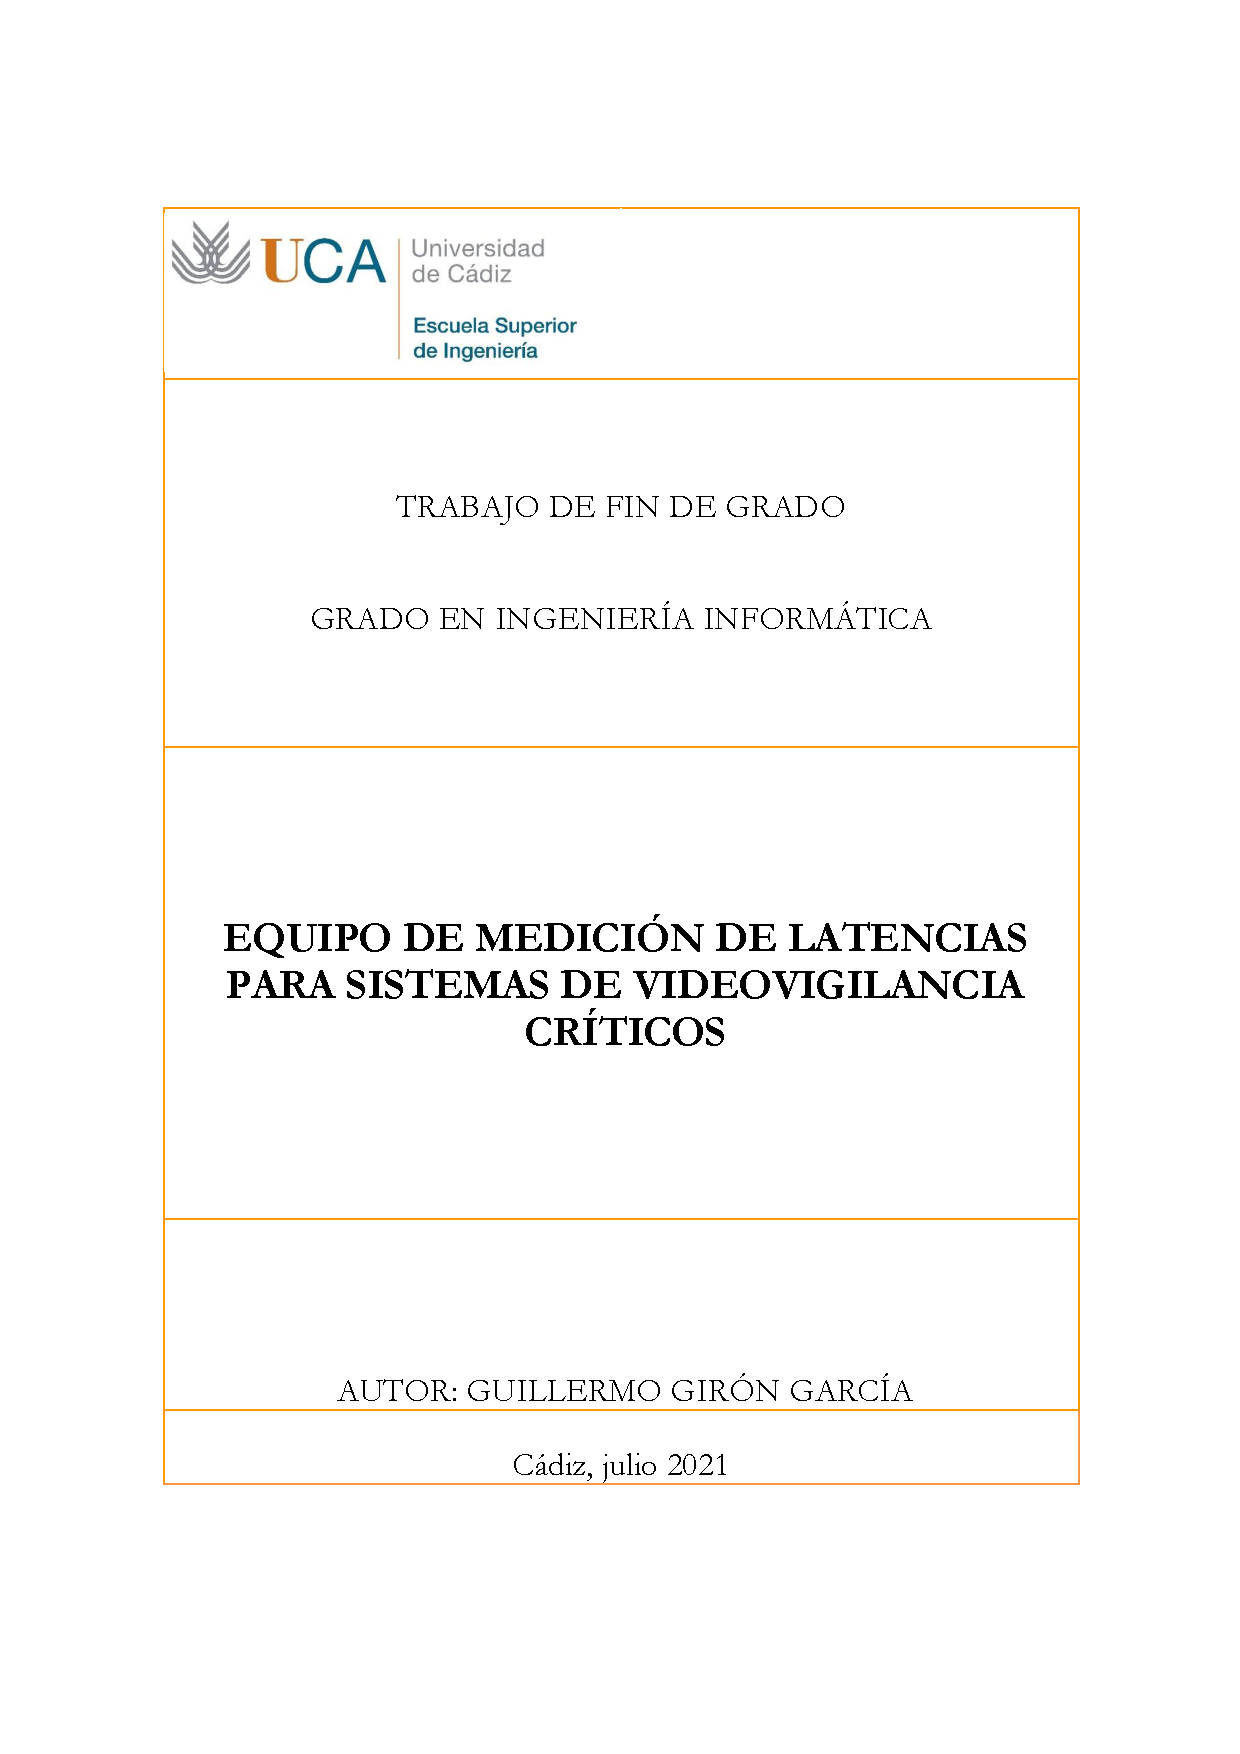
\includepdf{Documents/Portada-externa.pdf}

\end{titlepage}
\newpage{\pagestyle{empty}\cleardoublepage}  
{
  \thispagestyle{empty} 
  \centering
  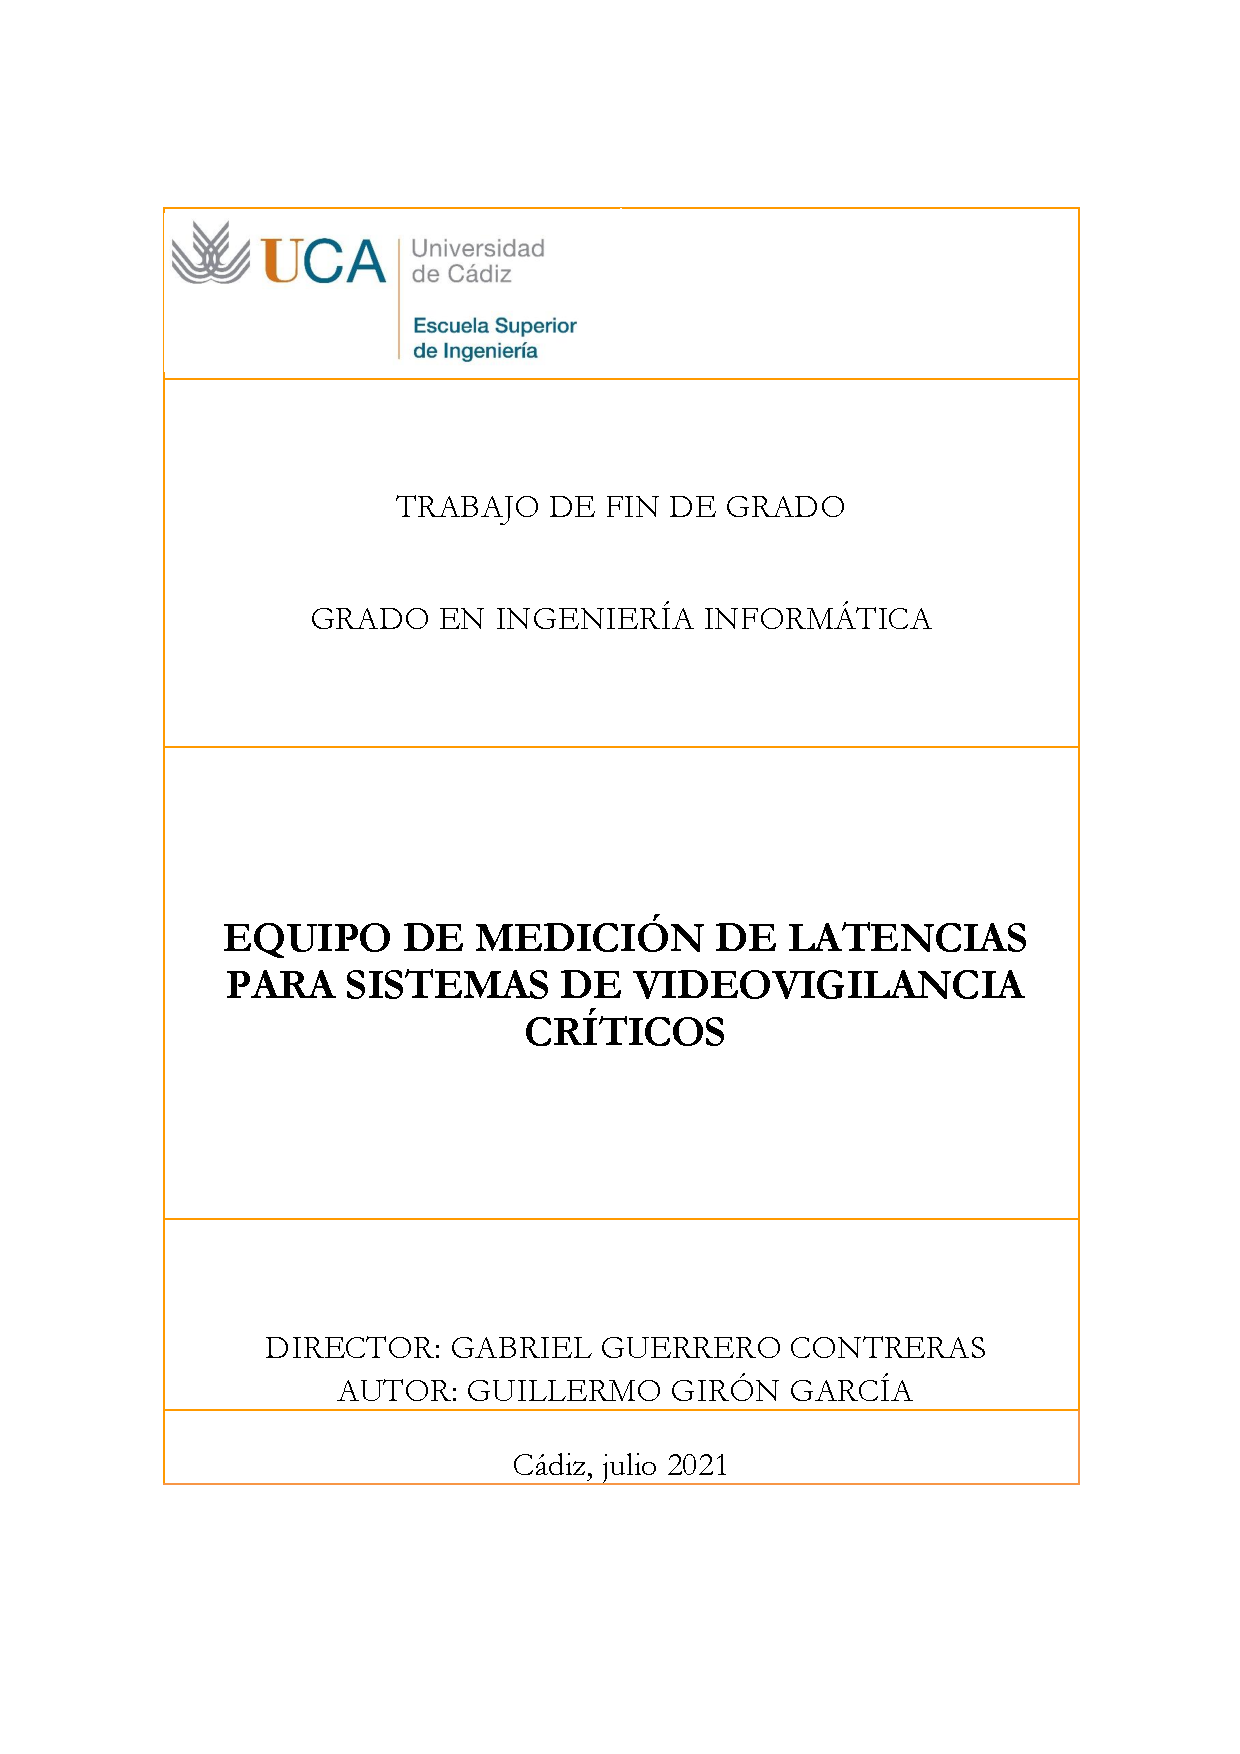
\includepdf{Documents/Primera-interna.pdf}
}

\clearpage
\newpage{\pagestyle{empty}\cleardoublepage}  
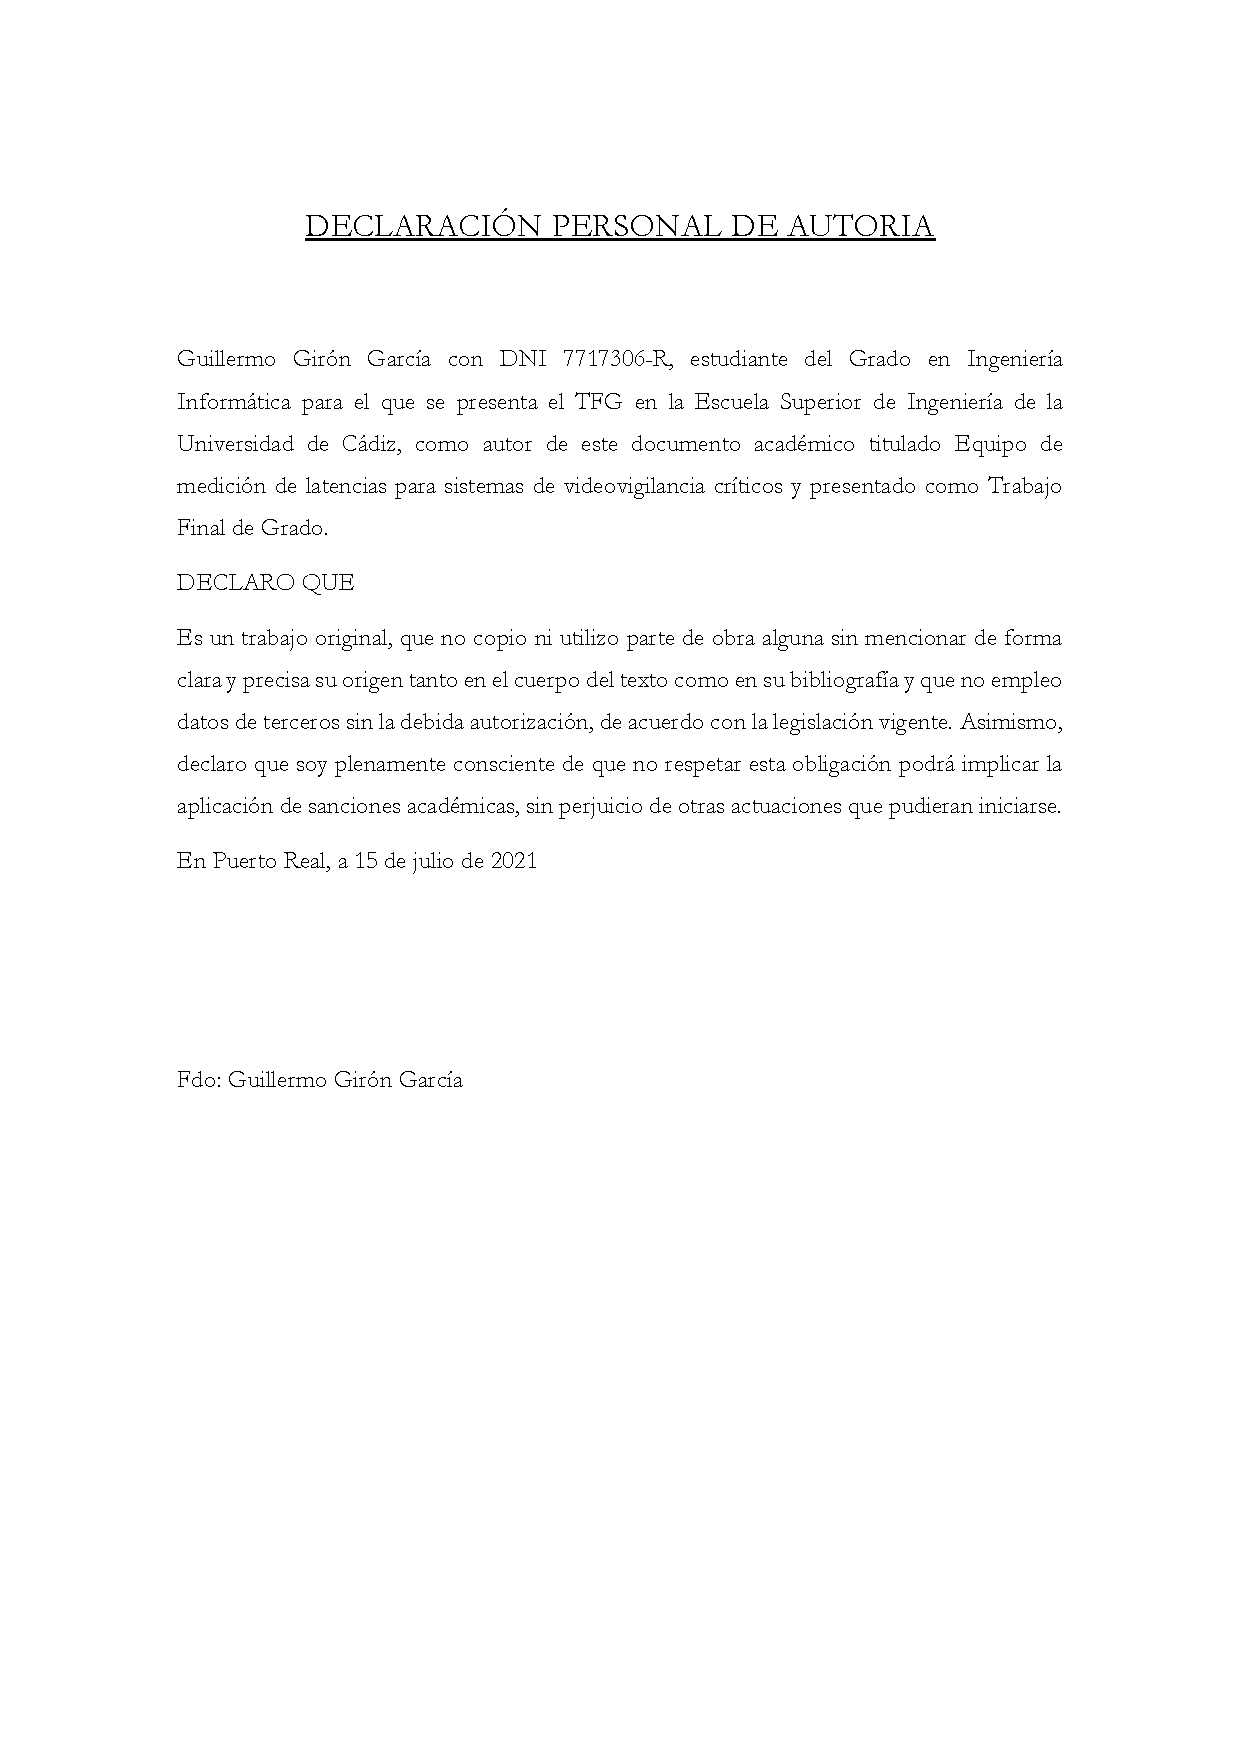
\includepdf{Documents/Segunda-interna.pdf}
\setcounter{page}{0}
\hypersetup{pageanchor=true}
\tableofcontents{}

\listoffigures

\listoftables


\chapter{Introducción\label{cap:introducci=0000F3n}}

Durante la lectura de este documento, le será presentado con todo lujo de detalles un dispositivo electrónico de nuevo desarrollo, cuyas aplicaciones, serán especialmente útiles en el ámbito militar y de la seguridad de entornos en tiempo real, pero que también puede tener aplicaciones en otros sectores, como la industria, donde puede ayudar a cuantificar y estandarizar así una medida, como es el retardo de vídeo.

Para comenzar, se dice que un sistema de videovigilancia es aquel que permite a través de la utilización de un circuito cerrado de televisión, la monitorización de vídeos e imágenes a distancia, con el objetivo de aumentar la seguridad de un entorno \cite{videovigilancia}.
 
A su vez, un sistema de videovigilancia es crítico cuando tiene que funcionar “en tiempo real”, es decir, ser capaz de captar una imagen, y mostrarla en un monitor con un tiempo de latencia suficientemente bajo como para que el operador de cámaras no tenga sensación de disonancia entre las entradas que recibe la cámara y el tiempo que tarda ésta en dar una respuesta a dichas entradas.

Se vuelve importante este hecho en entornos donde se conjugan un altísimo nivel de seguridad, con la necesidad de una respuesta muy rápida a cualquier evento que se produzca y pueda afectar a la misma.

Se contextualiza este concepto, en el hecho que se conoce como revolución digital, cuyo avance ha afectado enormemente a los dispositivos y medios de captación de imágenes y su posterior tratamiento y adecuación al medio en el que serán utilizadas.
 
Este proyecto pretende dar respuesta a si un sistema de videovigilancia es o no de tiempo real.
Consistirá en el desarrollo de un sistema de medición de latencias para sistemas de videovigilancia, que incluye un dispositivo de medición de bajo coste y alta efectividad, equipado con un software capaz de suplir las necesidades del personal técnico encargado de realizar dichas mediciones. 
 
Así mismo, se realizará una descripción de toda la metodología aplicada al realizar las mediciones, un completo análisis de todo el transfondo tecnológico del hardware utilizado durante el proyecto y se documentará el desarrollo e instalación del software que constituye el sistema de medición.

% \section*{Listados}

% Una opción es incluir directamente el código en el documento utilizando
% \emph{verbatim}: \begin{verbatim}
% epService.getEPRuntime().sendEvent(evento);
% \end{verbatim}

% \LaTeX{} también permite incluir listados desde ficheros de texto,
% ajustando automáticamente las líneas de código a la configuración
% especificada. Puede verse un ejemplo en el Listado~\ref{lst:enviarEvento}.

% \lstset{basicstyle=\footnotesize, frame=single, breaklines=true, tabsize=3}
% \lstinputlisting[caption=Envío de un evento a Esper, label=lst:enviarEvento]{enviarEvento.txt}

\section{Motivación}

Dado el actual auge de los sistemas digitales en todos los posibles ámbitos de la vida cotidiana, hay uno que ha destacado de sobre manera, y es la captación, tratamiento y visualización de las imágenes, y por ende, al vídeo.

Aplicada esta revolución digital al entorno de la defensa y seguridad, llegamos a los sistemas de videovigilancia modernos, los cuales aumentan la complejidad de los antiguos sistemas analógicos, añadiendo componentes electrónicos de diversa índole que son los encargados de conseguir una imagen digital de calidad, pero a que su vez, producen inherentemente un retardo en la consecución y retransmisión de la misma a través de un monitor.

La necesidad laboral y el interés de algunas empresas en el desarrollo de un producto, de bajo coste, y de eficacia probada son el motivo principal de este estudio.

Eso nos lleva hasta la idea de este estudio el cuál, pretende dar una herramienta sencilla y barata para medir dichos retardos y a la vez, establecer una serie de pautas generales las cuales para identificar que sistemas pueden ser considerados como críticos y cuales no, precisamente, en base a este criterio de medida que es su latencia de funcionamiento.

Se comenzará el desarrollo del sistema con la premisa de desarrollar un prototipo de producto funcional, el cuál, disponga entre sus características técnicas:

\begin{itemize}
    \item La capacidad de ser portátil y transportable.
    \item Funcionar utilizando una batería incorporada en lugar de conectado a una red de corriente.
    \item Tener una interfaz de usuario sencilla y amigable.
    \item Ser capaz de realizar mediciones precisas de las latencias de un sistemas de vídeo.
    \item Tener un bajo coste y estar desarrollado inicialmente con hardware open source.
\end{itemize}

Para ello, se ha comenzado revisando el estado del arte y la existencia de dispositivos similares en el mercado. Comercialmente, no se ha encontrado ninguno, y de fabricación casera, aunque usado profesionalmente, se ha encontrado un sistema similar, construido  por los ingenieros de la empresa sueca Voysys, con la salvedad de que no es portátil y solo trabaja bajo entorno Windows, dependiendo de un ordenador que realice los cálculos e inicie las mediciones. Este dispositivo es brevemente mostrado en un vídeo subido en el canal de Youtube de la compañía y no se proporciona información de como está construido, utilizando que componentes, como se conecta con el ordenador o que lenguaje se ha utilizado para su programación, pero a simple vista se puede observar que utiliza los mismos componentes que se pretenden utilizar en este proyecto conectados mediante una conexión serie o usb. Estos son:

\begin{itemize}
    \item Placa microcontroladora.
    \item Fotosensor.
    \item Led.
\end{itemize}

Estos dispositivos, que son los responsables de las mediciones en el sistema de Voysys, serán los encargados de tanto de tomar mediciones como de realizar los cálculos y representar las mismas para su visualización, y es por ello y por su condición de portátil por lo que se realizarán los siguientes cambios en los componentes:

\begin{itemize}
    \item SBC en lugar de placa microcontroladora.
    \item Se añadirá una batería.
    \item Pantalla táctil.
    \item Interfaz gráfica propia y adaptada integrada en un sistema operativo propio.
\end{itemize}

Respecto a la medición de latencias en sistemas de visión nocturna, se debe tener en cuenta que existe un amplio abanico de tecnologías disponibles actualmente, partiendo de las tradicionales con iluminación fosfórica verde a las modernas imágenes térmicas digitales. Pese a ello, no se ha encontrado nada similar al dispositivo que pretende desarrollar este proyecto. Teniendo en cuenta que todo lo relacionado a este ámbito de la vigilancia nocturna suele pertenecer al ámbito militar, es comprensible que haya menos información al respecto.

\section{Objetivos}

El objetivo de este proyecto es el desarrollo del software embebido que controlará un medidor de latencias para sistemas de videovigilancia críticos, así como su despliegue e instalación en el dispositivo hardware de destino. El producto final deberá ser funcional, sencillo de utilizar y operar sobre una plataforma hardware de bajo coste. Para lograr dicho objetivo se acometerán los siguientes puntos:

\begin{itemize}
    \item Describir las pautas y comportamientos que tiene un sistema de videovigilancia crítico.
    \item Estudiar cómo afectan los distintos componentes de un sistema de videovigilancia a su latencia.
    \item Establecer el proceso a seguir a la hora de medir distintos sistemas de videovigilancia con distintas características.
    \item Desarrollar el software capaz de coordinar los componentes del equipo de medición, calcular las latencias de un sistema de videovigilancia y representarlas gráficamente a través de una interfaz de usuario.
    \item Desplegar e instalar el software desarrollado en el dispositivo hardware de destino, verificando su correcto funcionamiento.
\end{itemize}

\section{Alcance}

El alcance de este proyecto se centra en el desarrollo, despliegue e instalación del software embebido del medidor de latencias. El producto hardware (placa, sensores, LED, batería, carcasa) será formalmente descrito y esquematizado en este documento, pero su diseño electrónico y fabricación física quedan fuera del alcance del mismo.

Se dará por concluido el proyecto cuando se tenga desarrollado el software del medidor de latencias con un funcionamiento eficaz y adecuado, instalado y desplegado correctamente sobre la plataforma hardware de destino, y además haya sido testado en diversas situaciones.

Respecto a los dispositivos de videograficos, se han mostrado de forma introductoria y no serán cubiertos en primera instancia por el alcance de este proyecto.

\section{Glosario}

\begin{description}
    \item [{Balance de blancos}] Ajuste de la cámara que sirve para equilibrar el nivel de los colores básicos, rojo verde y azul.
    \item [{Zoom}] Variación de la longitud focal y  ángulo de visión manteniendo el plano de la imagen en el mismo sitio.
    \item [{Resolución}] Cantidad de detalles que pueden apreciarse en una imagen. Medida en píxeles. 
    \item [{Apertura}] Indica la luminosidad del objetivo que incorpora la cámara.
    \item [{ISO}] Sensibilidad que tiene el sensor de la cámara para captar luz.
    \item [{Fotones}] Partículas con energía lumínica.
\end{description}

\subsection{Acrónimos}

\begin{acronym}
  \label{acro}  
  \acro{PFC}{Proyecto Fin de Carrera}
  \acro{UCA}{Universidad de Cádiz}
  \acro{SVC}{Sistema de videovigilancia crítico}
  \acro{CCTV}{Circuito de televisión cerrado}
  \acro{NIR}{Near Infrared - Cercano al infrarrojo}
  \acro{PPP}{Pixels por pulgada}
  \acro{CMOS}{Semiconductor complementario de óxido metálico}
  \acro{CCD}{Dispositivo de carga acoplada}
  \acro{MCP}{Placa de microcanales}
  \acro{GaAs}{Arseniuro de gallio}
  \acro{CRA}{Central receptora de alarmas}
  \acro{SBC}{Ordenador en una unica placa}
  \acro{ARM}{Maquina RISC Avanzada}
  \acro{RISC}{Conjunto reducido de instrucciones de computación}
  \acro{USB}{Bus de serie universal}
  \acro{SOC}{Sistema en chip}
\end{acronym}

\chapter{Transfondo tecnológico}

En este capítulo se darán a conocer las tecnologías con las que se trabajará durante el transcurso del documento y el desarrollo del producto de cara a ilustrar sus contextos históricos y motivación de uso.

\section{Comienzos}

A finales del siglo XIX, alrededor del 1880 surgen las vídeo cámaras \cite{gray1993multiformat}, con fines cinematográficos, y es desde entonces, que son dispositivos que no han dejado de evolucionar, tanto en forma, como en calidad, funcionalidad o tamaño.

\hfill\break
A mitad del siglo XX, en 1942, nace en plena segunda guerra mundial, el termino que acuñamos como vídeovigilancia, de la mano del primer circuito de televisión cerrado o CCTV. Fue en este momento, cuando se comenzó a utilizar un sistema videográfico \enquote*{a tiempo real} como elemento de seguridad en un entorno crítico \cite{fan2015survey}. Ver Figura \ref{fig:cctv_simple}.

\begin{figure}[H]
    \centering
    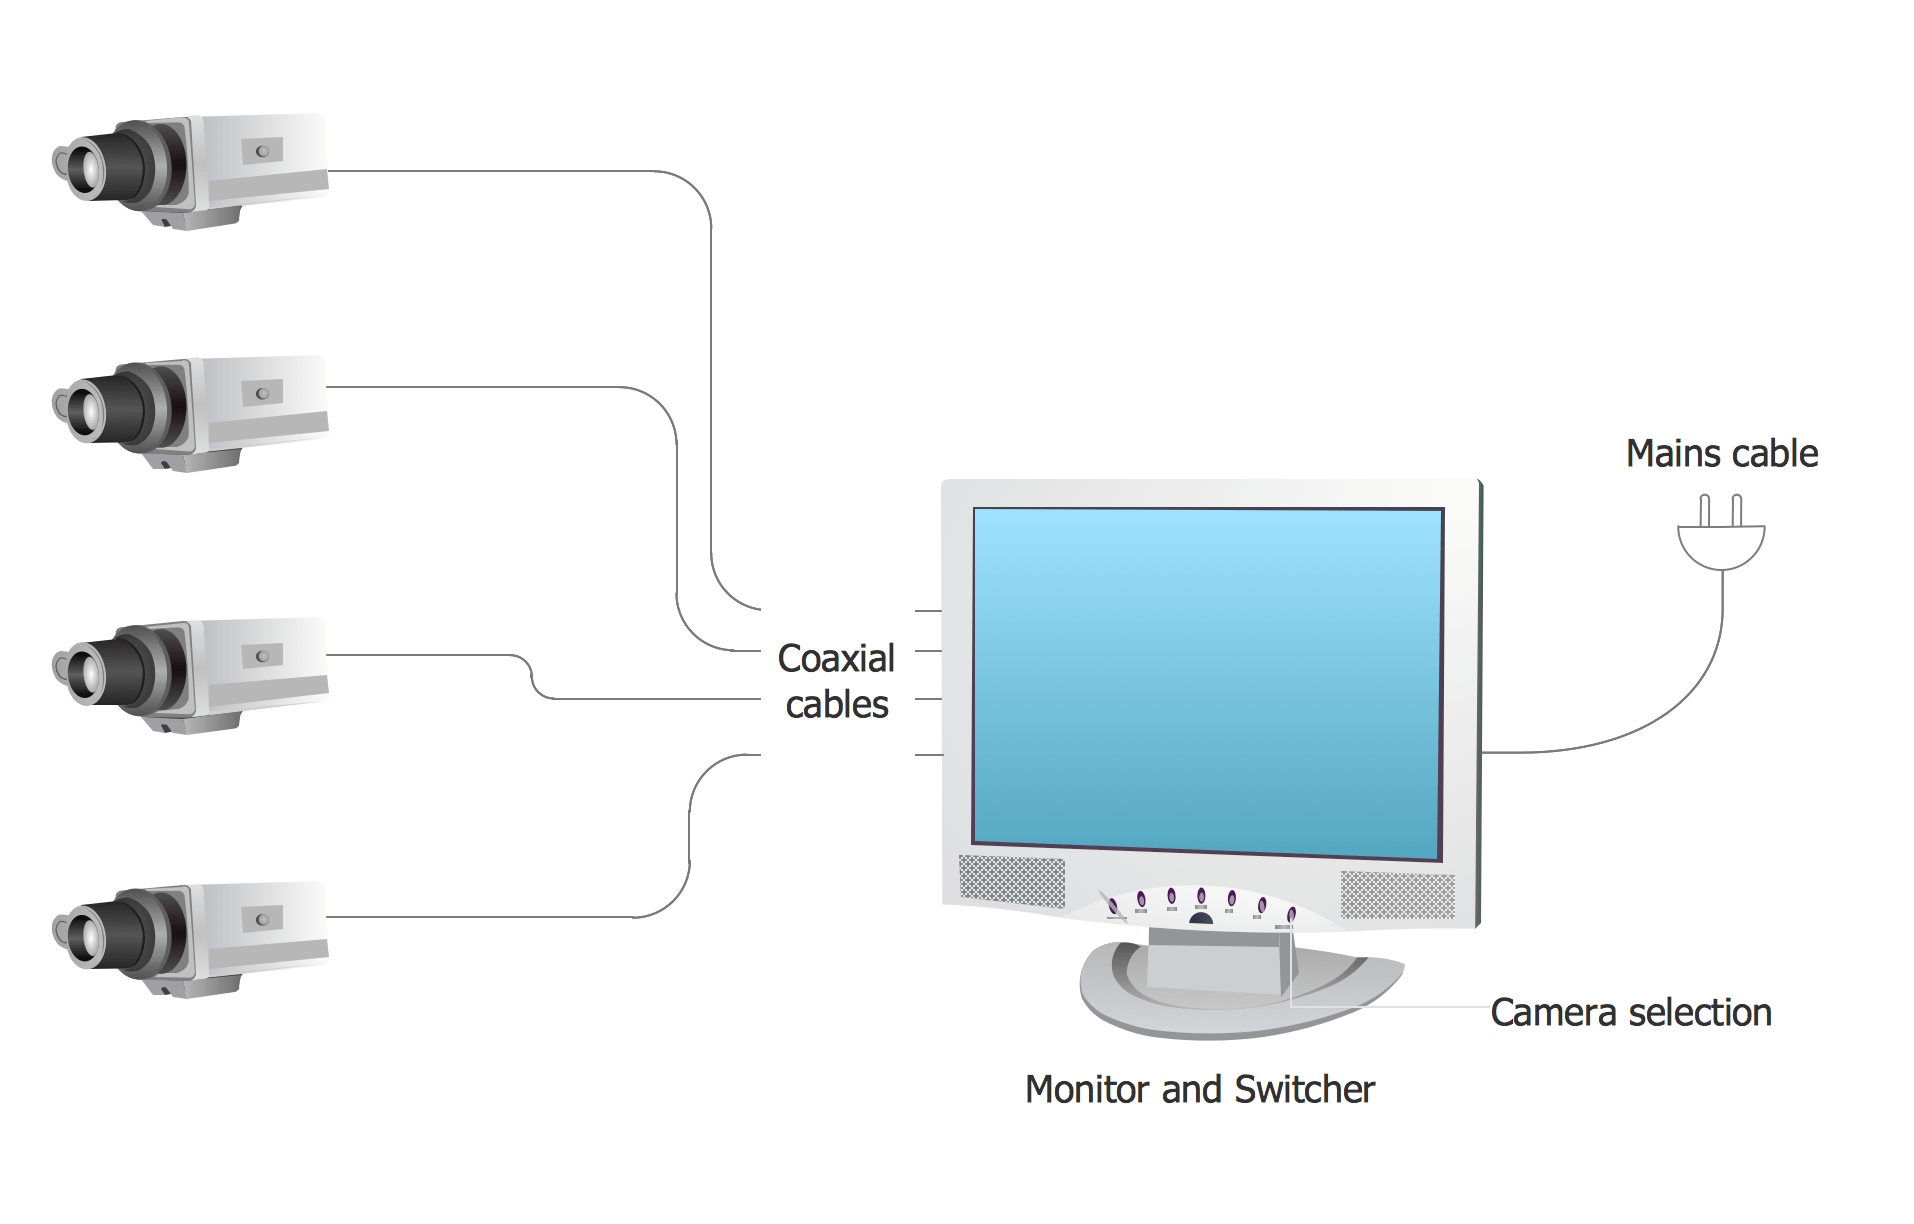
\includegraphics[scale = 0.44]{Figures/Simple_CCTV.png}
    \caption{CCTV Simple con 4 cámaras conmutadas. Fuente: \cite{cctv_4}}
    \label{fig:cctv_simple}
\end{figure}

Al principio, estos circuitos de televisión eran enormemente sencillos, y solo incluían cámaras en blanco y negro conectadas a monitores remotos, que eran a su vez utilizados, para controlar el lanzamiento de cohetes. Desde entonces, y hasta la fecha, los avances en vídeo vigilancia han tenido un enorme auge, y han propiciado el desarrollo de nuevas tecnologías que han ido escalando a la vez que estos sistemas.

\hfill \break
En un principio, los CCTV, requerían de supervisión humana constante para funcionar y ser eficaces, pero con el paso de los años y la invención de las cintas de vídeo se facilitó el proceso de vigilancia, gracias a poder grabar lo que sucedía en las cámaras. Ver Figura \ref{fig:cctv_recorder}.

\begin{figure}[H]
    \centering
    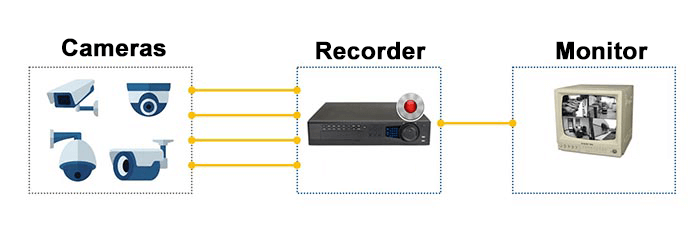
\includegraphics[scale = 0.81]{Figures/cctv_con_grabacion.png}
    \caption{CCTV con sistema de grabación. Fuente: \cite{cctv_4}}
    \label{fig:cctv_recorder}
\end{figure}

Poco después, en los años 60's, se comenzó a popularizar el uso de cámaras de vídeo vigilancia en lugares públicos, situándolas en puntos estratégicos, los cuales permitían aprovechar al máximo sus recursos, e incluso pasar desapercibidas en muchos casos\cite{videovigilancia_historia:2017:Online}. 

\hfill \break
Unos años más tarde, este boom de la vídeo vigilancia, comienza a afectar a otros sectores de la sociedad, y se populariza, la utilización de CCTV's en otros lugares, como bancos y tiendas, utilizándose como una medida de seguridad añadida antirrobos. Es gracias a este auge, que al igual que sucedió en el sector de la informática, con las cámaras de vídeo vigilancia, se fueron mejorando enormemente las características de los sistemas, abaratando costes, reduciendo sus tamaños, y mejorando la visibilidad en situaciones de poca luz, lo que conllevó con el paso de los años a su irrupción en el mercado doméstico como una medida para mantener a las familias seguras disuadiendo a posibles invasores del hogar.

\section{Visión Nocturna}

Se conoce como visión Nocturna al fenómeno de poder vislumbrar en ausencia de luz, el entorno que nos rodea, y no resulta nada nuevo. Desde mucho tiempo atrás, se sabe que ciertos animales, como son los búhos, los gatos, pueden ver en la oscuridad y otros como las abejas, incluso llegan a detectar partes del espectro visible que son invisibles al ojo humano. Este fenómeno tiene cabida, al ser estos animales capaces de detectar con sus ojos frecuencias del espectro electromagnético que nosotros no podemos \cite{sionyx_night_vision}. 

\begin{figure}[H]
    \centering
    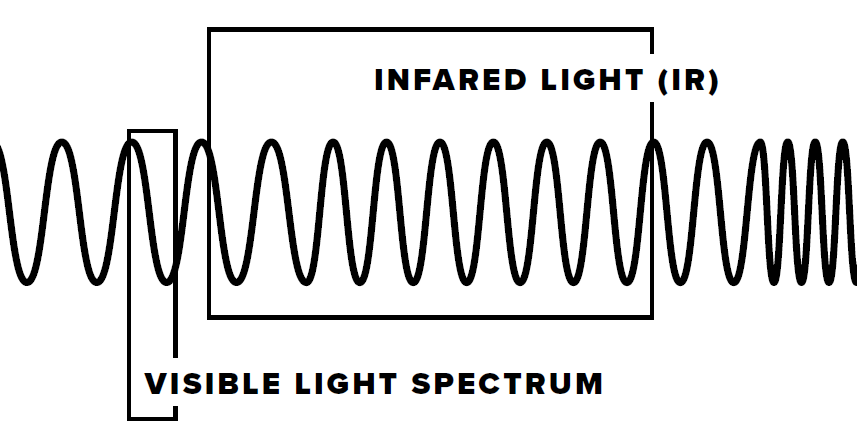
\includegraphics[scale = 0.5]{Figures/espectro_luminoso.PNG}
    \caption{Espectro luminoso visible + infrarrojo. Fuente: \cite{spectre}}
    \label{fig:espectre}
\end{figure}

Durante la segunda guerra mundial y sucesivas, se comenzaron a desarrollar y utilizar distintas soluciones técnicas, que permitían a los soldados, operar en completa oscuridad, imitando con ellas, el comportamiento de la visión animal \cite{tsuji2002development}. No mucho más tarde, se aplicarían estas técnicas a la vídeo vigilancia, añadiendo estos dispositivos a vídeo cámaras de un CCTV, en forma de filtros o sensores, dando así lugar a las primeras cámaras de visión nocturna.

\break

Esencialmente, podríamos clasificar los tipos de visión nocturnas utilizados en la actualidad en cuatro \cite{chrzanowski2013review}:

\begin{itemize}
    \item Visión nocturna analógica: mediante un tubo intensificador de luz con fósforo y una batería.
    \item Visión nocturna digital: utiliza sensores fotográficos ultrasensibles y postprocesado de imágenes para proyectar una imagen nítida.
    \item Visión térmica: basada en la detección de la radiación infrarroja.
    \item Dispositivos novedosos: destacan por el auge de una nueva tecnología que incorpora la utilización de visión nocturna digital y analógica para la reducción de ruido en la señal de imagen.
\end{itemize}

\subsection{Visión nocturna analógica}

Comenzaremos explicando la principal morfología común que comparten casi todos los dispositivos de visión nocturna analógicos. Dichos componentes se conocen como:

\begin{itemize}
    \item Lentes objetivo.
    \item Una pieza ocular.
    \item Fuente de alimentación.
    \item Un tubo intensificador de imágenes.
\end{itemize}

La visión nocturna, en este caso, surge durante la intensificación de la imagen en el tubo intensificador, el cuál cuenta con dos subcomponentes principales que son los que se encargan de mejorar la imagen. Estos son:

\begin{itemize}
    \item \textbf{Fotocátodo} Absorbe fotones y libera electrones.
    \item \textbf{Fotomultiplicador} Absorbe electrones, los multiplica y libera fotones intensificados o multiplicados.
\end{itemize}

A continuación se detalla como funciona la visión nocturna analógica. Al frente de cualquier dispositivo, se encuentran las lentes objetivo, cuyo trabajo consiste en reunir toda energía infrarroja ambiental y artificial disponible antes de enviarla al tubo de amplificación. Este tubo tiene forma de túnel y está alimentado electrónicamente.
Todos estos fotones captados, pasan a trace de un fotocátodo, el cuál los convierte en electrones. Estos electrones se mueven hacia una placa de micro canales, donde son amplificados por un factor de miles a través de una de reacción eléctrica y química en cadena que se produce cuando estos electrones impactan en las paredes de los micro canales. Ver Figura \ref{fig:analog_intensification}.

\begin{figure}[H]
    \centering
    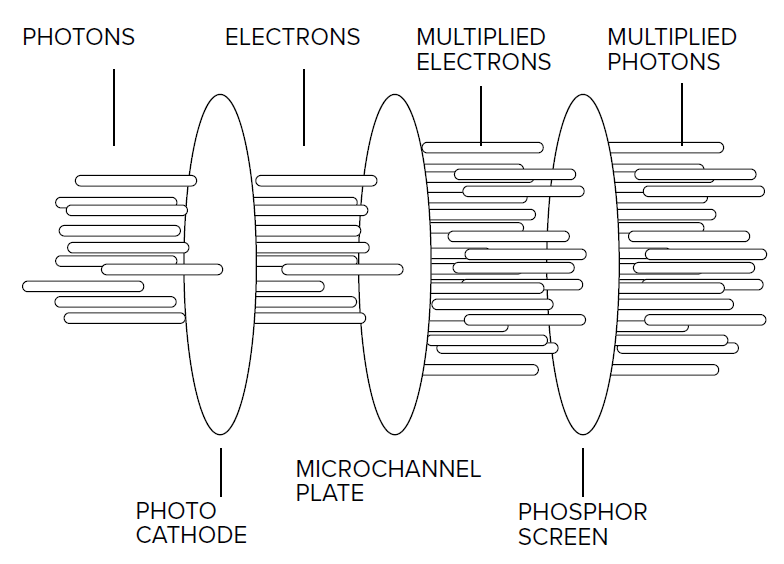
\includegraphics[scale = 0.5]{Figures/amplificacion_analogica.PNG}
    \caption{Amplificación analógica de fotones. Fuente: \cite{intensifier}}
    \label{fig:analog_intensification}
\end{figure}

Estos electrones supercargados, son golpeados en una pantalla cubierta de fósforo donde alcanzan un estado de excitación, liberando así nuevas partículas fotónicas o de luz visible las cuales pueden verse a través de una pieza ocular. La imagen aparecerá como una recreación clara y lúcida de la escena que estamos observando, pero en una combinación de tonos verdes y negros.

El motivo de que el color de imagen sea verde o verdoso viene del uso de la pantalla de fósforo, el cuál se utiliza a su vez por una sencilla razón, y es que el ojo humano es muy sensible a los tonos verdes y puede distinguir más formas de verde que de ningún otro color en el espectro. Ver Figura \ref{fig:analog_vision}

\begin{figure}[H]
    \centering
    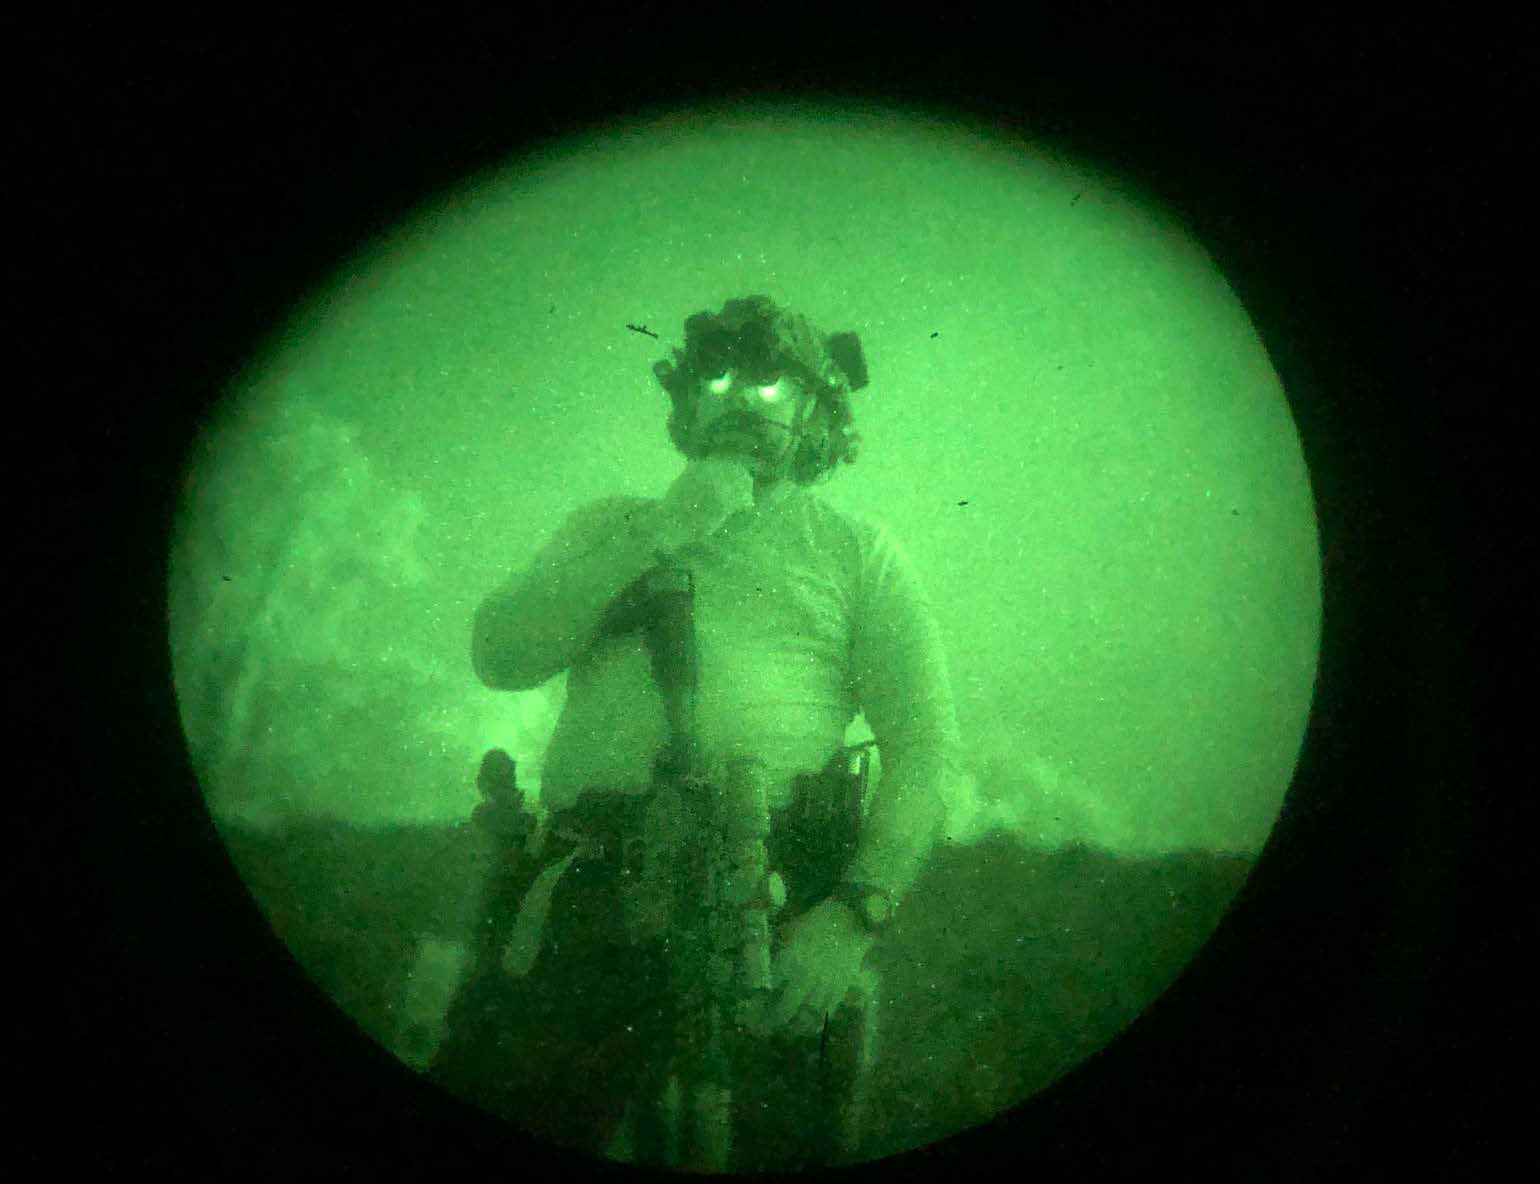
\includegraphics[scale = 0.25]{Figures/vision_amplificacion_analogica.png}
    \caption{Ejemplo de visión nocturna analógica. Fuente: \cite{sionyx_night_vision}}
    \label{fig:analog_vision}
\end{figure}

\subsection{Visión nocturna digital}

Los dispositivos de visión nocturna digital operan de manera diferente a los analógicos. En su lugar, la luz que captan las lentes objetivo, es transformada en una señal digital mediante un sensor de imagen que puede variar entre dos tipos:

\begin{description}
        \item [{CMOS}] Complementary Metal Oxide Semiconductor
        \item [{CCD}] Charge Coupled Device
\end{description}

Estas son las mismas tecnologías empleadas en todas las cámaras digitales domésticas. 
En ellas, la imagen es mejorada varias veces antes de ser visible en las pantallas de los dispositivos. Cuanto más grandes los tamaños de píxeles de los sensores CMOS o CCD, mejor rendirán en entornos de baja luminosidad.
En este tipo de dispositivos se utilizan y desarrollan tecnologías de sensores que funcionan en el espectro NIR, consiguiendo así imágenes con nitidez, pero que en ausencia de luz, se representan con aberraciones cromáticas. Se los conoce como dispositivos "low light".

Como desventaja frente a sistemas analógicos tradicionales, presentan una muy baja resolución de imagen, ya que al tener píxeles muy grandes, apenas se pueden introducir entre uno y dos megapíxeles en un sensor.
Como ventaja, tienen un menor coste y una enorme capacidad para superponer iconos, indicadores y otra información de valor sobre la imagen proyectada. Ver Figura \ref{fig:digital_vision}.

Ya que estos dispositivos convierten imágenes ópticas en señales digitales, son dispositivos que tienen la posibilidad nativa de grabar vídeo, imágenes y sonido, el cuál puede ser almacenado a bordo fácilmente en una memoria, serán los principalmente utilizados durante el estudio y pruebas de éste proyecto.

\begin{figure}[H]
    \centering
    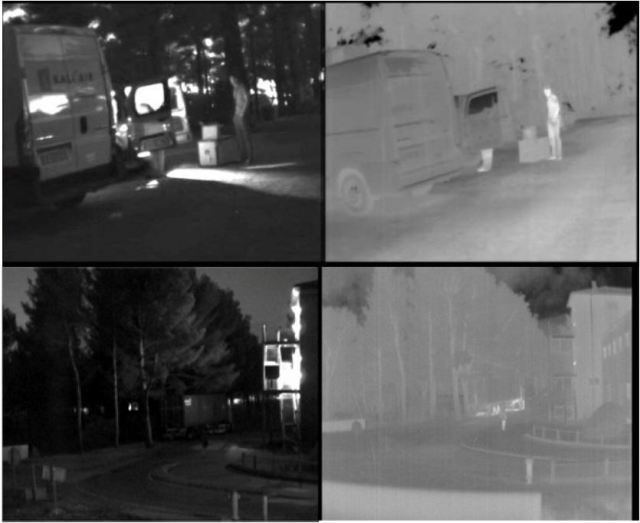
\includegraphics[scale = 0.7]{Figures/low_light_example.jpg}
    \caption{Ejemplo de visión low light (izquierda) vs térmica (derecha). Fuente: \cite{night_vision}}
    \label{fig:digital_vision}
\end{figure}

\subsection{Visión Artificial}

En la actualidad, los dispositivos de visión nocturna van equipados con un nivel de tecnología enorme, pero aún con él, en condiciones de apagón total, en ausencia completa de radiación lumínica, siguen sin ser más útil que un ojo humano sin ayudas. Es aquí donde aparece el \textbf{iluminador infrarrojo}. Ver Figura \ref{fig:ir_iluminator}.

\begin{figure}[H]
    \centering
    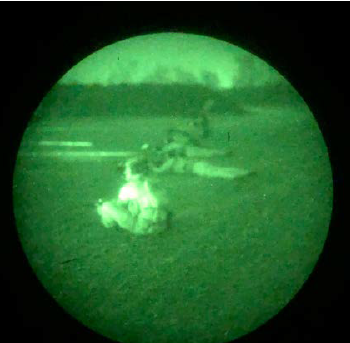
\includegraphics[scale = 0.8]{Figures/no_ir_iluminator.PNG}
    \caption{Ejemplo de visión sin iluminador infrarrojo. Fuente: \cite{sionyx_night_vision}}
    \label{fig:no_ir_iluminator}
\end{figure}

Como ocurre en los ya mencionados dispositivos, analógicos y digitales, todos los aparatos de visión nocturna deben tener alguna luz que amplificar. Existen situaciones donde simplemente no existe suficiente luz para que un amplificador de luz las intensifique. Ejemplos de ellas pueden ser:

\begin{itemize}
    \item Estructuras subterráneas.
    \item Cuevas.
    \item Noche nublada sin luna.
\end{itemize}

\begin{figure}[H]
    \centering
    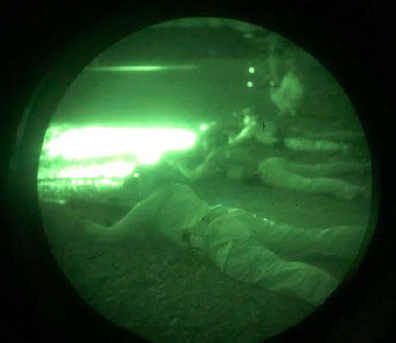
\includegraphics[scale = 0.75]{Figures/ir_iluminator.PNG}
    \caption{Ejemplo de visión con iluminador infrarrojo. Fuente: \cite{sionyx_night_vision}}
    \label{fig:ir_iluminator}
\end{figure}

En estas situaciones, es cuando el iluminador infrarrojo entra en acción. Se trata de un dispositivo que provee de iluminación artificial de una longitud de onda apropiada cercana al espectro infrarrojo que permite al usuario iluminar áreas de interés específico mientras además mejoran el contraste de la imagen.
Se puede interpretar como una linterna invisible que solo puede ser vista a través de un dispositivo de visión nocturna. En las siguientes figuras se mostrarán tres ejemplos de visión con iluminador infrarrojo (Figura \ref{fig:laser_ir_iluminator} y sin él ver Figura \ref{fig:no_ir_iluminator}).

\begin{figure}[H]
    \centering
    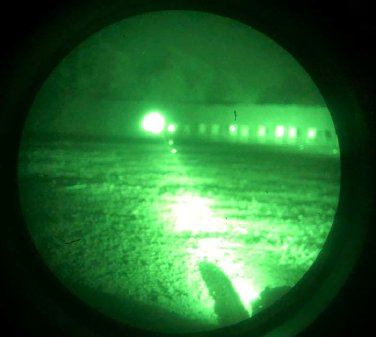
\includegraphics[scale = 0.7]{Figures/laser_ir_iluminator.PNG}
    \caption{Ejemplo de visión con iluminador infrarrojo láser}
    \label{fig:laser_ir_iluminator}
\end{figure}

\subsection{Clasificación de los dispositivos de visión nocturna en generaciones}

Comúnmente se clasifican en tres generaciones para facilitar la segmentación según su tecnología. Esta clasificación es dada por el Ejercito de Estados Unidos \cite{kotulak1992methods}.

\subsubsection{Primera Generación}

El primer sistema de visión nocturna fue creado por la Armada de los Estados Unidos y utilizado durante la segunda guerra mundial. Este sistema dependía enteramente de una fuente de iluminación infrarroja para funcionar. La tecnología desarrollada llevó a lo que se conocen como Starlight Scopes (Visores de estrellas), popularizados en la década de 1960 y utilizados durante la guerra de Vietnam.
Siendo dispositivos arcaicos, se caracterizaban por ser capaces de proveer una imagen utilizable en todo entorno ayudados de un iluminador infrarrojo, del cual eran capaces de prescindir en las noches de luna llena sin nubes, y de proporcionar imágenes plagadas de ruido eléctrico. Ver Figura \ref{fig:starlight_scope}.

\begin{figure}[H]
    \centering
    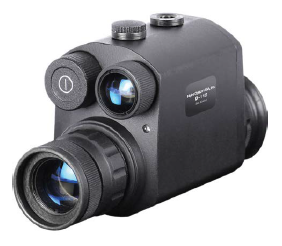
\includegraphics[scale = 1]{Figures/first_gen.PNG}
    \caption{Ejemplo de Starlight Scope. Fuente: \cite{sionyx_night_vision}}
    \label{fig:starlight_scope}
\end{figure}

\subsubsection{Segunda Generación}

Se considera como primordial diferencia en este cambio generacional la incorporación de una placa de microcanales (MCP) al tubo intensificador de imágenes. Un MCP es un disco de vidrio recubierto de metal que multiplica los electrones producidos por el intensificador de imágenes y que además, elimina la distorsión. Adicionalmente, el número de agujeros, o canales, es un factor contribuyente en la determinación de la resolución. Ver Figura \ref{fig:second_gen}.

Los MCP, actuan como un supercargador de electrones y se encuentran localizados detrás del fotocátodo. Consisten en miles de orificios paralelos en el vidrio. A medida que los electrones pasan a través de estos tubos, miles de electrones adicionales se liberan, permitiendo a la luz ser amplificada muchas más veces que en los dispositivos de primera generación. Con esto al final, se consiguen mejores imágenes. Ver Figura \ref{fig:second_gen_example}.

\begin{figure}[H]
    \centering
    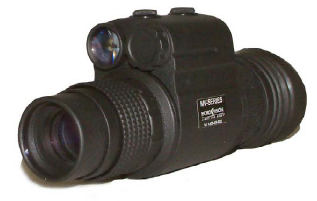
\includegraphics[scale = 1]{Figures/second_gen.PNG}
    \caption{Ejemplo de dispositivo de segunda generación. Fuente: \cite{sionyx_night_vision}}
    \label{fig:second_gen}
\end{figure}

\subsubsection{Tercera Generación}

Son dispositivos que se benefician primordialmente de la utilización de un material semiconductor, conocido como arseniuro de gallio (GaAs), añadido al proceso de fabricación del fotocátodo contenido en el tubo intensificador de imagen. La adición del GaAs, ayuda en la consecución de imágenes aún más brillantes, y más nítidas, gracias a su alto nivel de eficiencia en convertir fotones en electrones, mejorando así la detección de objetos a mayores distancias, en condiciones lumínicas más adversas.

Otro hito de esta generación es la inclusión de una película de iones, que actúan como barrera incrementando la vida útil del tubo intensificador de imágenes y protegiéndolo de fuentes de luz adversas.

\begin{figure}[H]
    \centering
    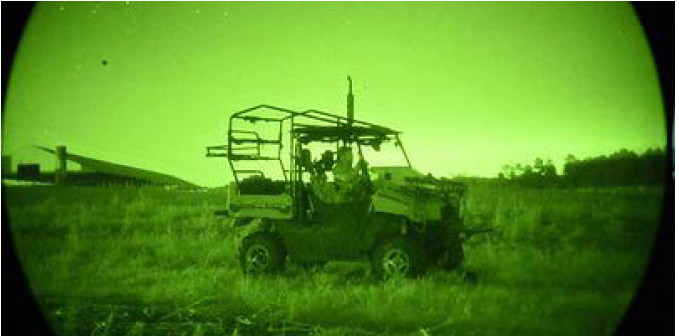
\includegraphics[scale = 0.8]{Figures/second_gen_example.PNG}
    \caption{Ejemplo de visión a con dispositivo de segunda generación. Fuente: \cite{sionyx_night_vision}}
    \label{fig:second_gen_example}
\end{figure}

Los dispositivos de visión nocturna de tercera generación típicos, ven resoluciones de aproximadamente 64 a 72 pares de lineas por milímetro y se benefician de una fuente de alimentación de alto voltaje. Los más actuales, también utilizan una fuente de alimentación cerrada, comúnmente conocida como Autogating. Esta fuente provee de rendimiento aumentado en entornos urbanos donde existen condiciones excesivas de luz ambiental, la cuales, crean lo que comúnmente se conoce como efecto blooming o halo. Este efecto consiste en la pérdida de porciones o de la misma imagen completa, debido a sobrecargas por una fuente de luz brillante, que blanquean la imagen.
El autogating minimiza las interferencias de estas luces brillantes encendiéndose y apagándose a un ritmo que es indetectable para el usuario incrementando así la efectividad de estos dispositivos en entornos urbanos. Ver Figura \ref{fig:third_gen}.

\begin{figure}[H]
    \centering
    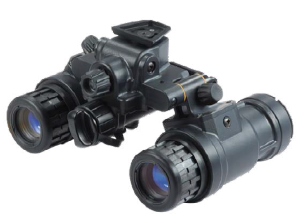
\includegraphics[scale = 1]{Figures/thrid_gen.PNG}
    \caption{Ejemplo de dispositivo de tercera generación. Fuente: \cite{sionyx_night_vision}}
    \label{fig:third_gen}
\end{figure}

\subsubsection{Fósforo blanco, pseudo cuarta generación}

Los dispositivos de cuarta generación per se, no existen ya que el Ejercito de Estados Unidos no ha dado aún tal designación. Dicho lo cual, los dispositivos sin películas de iones con fósforo blanco, son el pináculo de actual de la tecnología de visión nocturna analógica.
Estos dispositivos equipan un MCP sin película que proveen un ratio mucho más alto de señal-ruido que los típicos dispositivos de tercera generación, reduciendo así el ruido estático o electrónico en condiciones muy oscuras.

Estas unidades de fósforo blanco ofrecen un nivel de detalle incrementado, mayor contraste y rango de tonos. La imagen azulado cálido también ofrece mayor gama de intensidad, resultante en mejor percepción de profundidad que con los tradicionales dispositivos de fósforo verde. En uso prolongado, parecen reducir también la fatiga ocular y los dolores de cabeza comparados con sus homólogos de verde. Ver figura \ref{fig:white_phosphore}.

\begin{figure}[H]
    \centering
    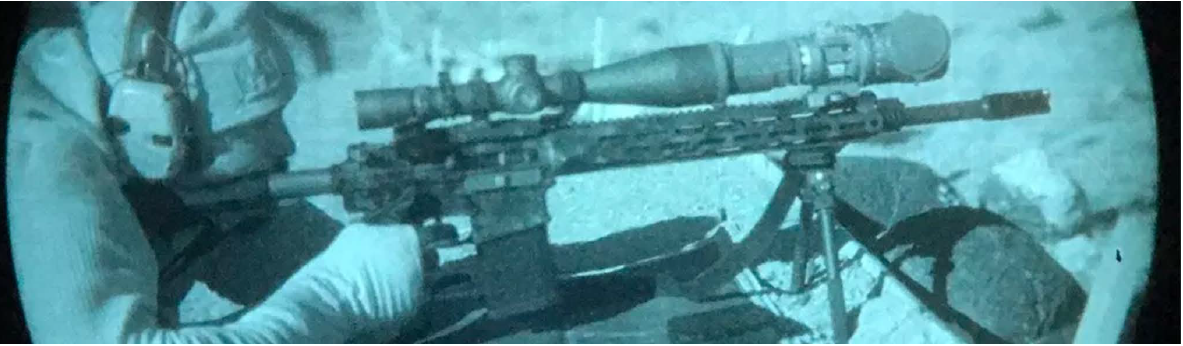
\includegraphics[scale = 0.4]{Figures/thrid_gen_example.PNG}
    \caption{Ejemplo de dispositivo con fósforo blanco. Fuente: \cite{white_phosphore}}
    \label{fig:white_phosphore}
\end{figure}

\subsubsection{Visión Térmica}

Podríamos considerar la visión Térmica como una subcategoría de la visión nocturna, ya que es una de las principales técnicas utilizadas en la actualidad cuando se trata de realizar videovigilancia en entornos de baja visibilidad.

\begin{figure}[H]
    \centering
    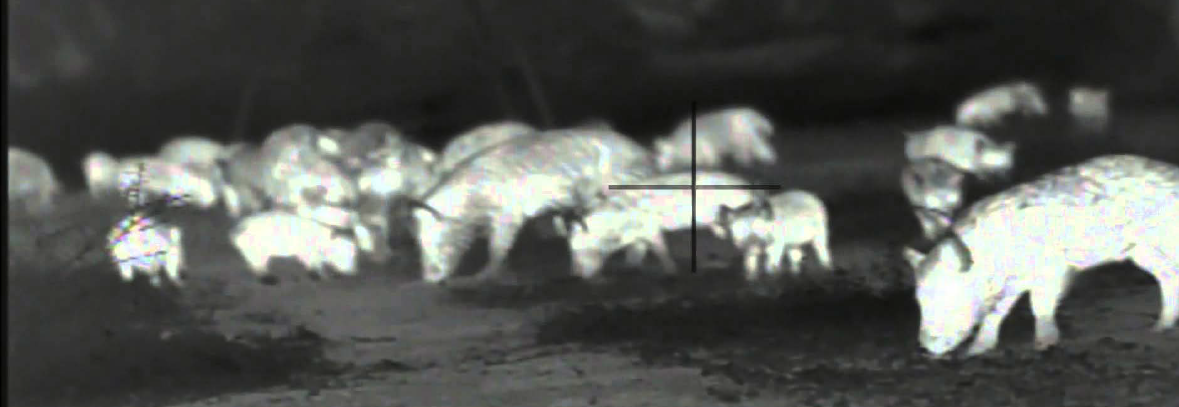
\includegraphics[scale = 0.4]{Figures/thermal_example.PNG}
    \caption{Ejemplo de dispositivo con fósforo blanco. Fuente \cite{thermal}}
    \label{fig:thermal_example}
\end{figure}

En estos dispositivos, en lugar de buscar luz que amplificar, se detecta radiación infrarroja mediante microbolómetros que cambian su resistencia basándose en la temperatura. Este cambio de microbolómetros puede ser medido y convertido a una imagen visible en miles de píxeles.
Para su funcionamiento se parte de la base de que todo objeto emite algún nivel de luz infrarroja. A más caliente esté el objeto, más radiación emitirá y más cambiará la luz, la resistencia de cada bolómetro.

La resolución de estos dispositivos está bastante por detrás de los dispositivos de visión nocturna actuales, aún así, las distancias de detección de objetivos son típicamente mayores. La regla general es que cuanto mayor sea la resolución, más capaz será la unidad y más va a costar económicamente. También, como la resolución en este caso es más baja que en los dispositivos de visión nocturna, sus imágenes son más dificiles de interpretar y dificultan el reconocimiento de objetos y paisajes. Para más inri, si todos los objetos de la escena se encuentran a similar temperatura, habrá poco contraste entre ellos. Ver figura \ref{fig:thermal_example}.

\section{Video vigilancia IP}

Se conoce como vídeo vigilancia IP a aquella tecnología de seguridad que permite la observación mediante cámaras de vídeo pertenecientes a un CCTV, en red, utilizando para ello internet y protocolos de interconexión. Con ello se consigue la transmisión y supervisión remotas de vídeo a distancia aún sin estar conectado directamente al CCTV \cite{norris2004growth}.

Esta tecnología, que es de alta implantación y utilización en la actualidad, aprovecha el cableado de red local existente para la interconexión de cámaras del circuito e incluso pueden transmitir las imágenes al exterior de la red local por medio de un ISP, permitiendo una transmisión de imágenes en línea. Con ello, se ahorra parte del coste del cableado que utilizan los CCTV y se re-aprovecha en muchos casos el ya existente de red. Otra posible ventaja que ofrecen, es la completa eliminación de cables y la transmisión de vídeo mediante tecnologías inalámbricas \cite{ipvm}.

Entre sus posibles usos, aparte de como cámaras de seguridad tradicionales, en la actualidad se la utiliza principalmente en aplicaciones de adquisición de datos mediante inteligencia artificial, ya que al ser cámaras digitales conectadas a una red donde puede haber ordenadores, resulta más sencillo tratar directamente las imágenes que estas captan.

\begin{figure}[H]
    \centering
    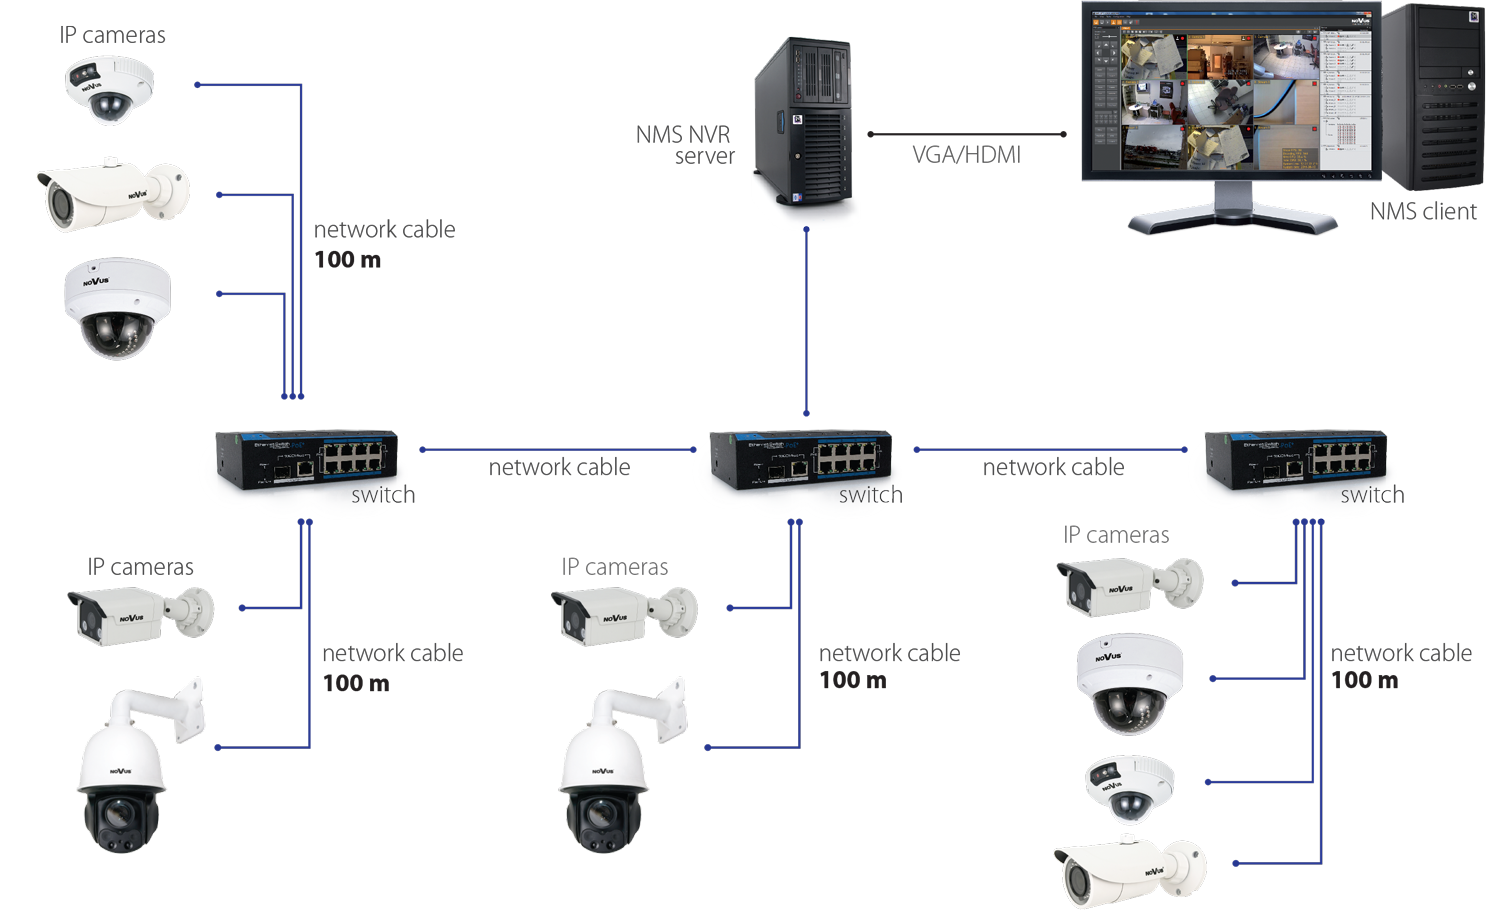
\includegraphics[scale = 0.2]{Figures/ip_cctv.png}
    \caption{Esquema de sistema de videovigilancia IP distribuido. Fuente: \cite{novus}}
    \label{fig:ip_cctv_example}
\end{figure}

\section{Comparativa de Hardware}
\label{hardware}

\begin{table}[H]
\caption{Comparativa de placas programables}
\label{tab:hardware}

\small
\begin{longtable}[c]{|c|p{5cm}|p{5cm}|}
\toprule 
&\textbf{Arduino} & \textbf{Raspberry Pi}\tabularnewline
\midrule
\midrule 
Tipo de hardware & Hardware libre  & Hardware propietario\tabularnewline
\midrule 
Arquitectura CPU & Microcontrolador ATMEL & Microprocesador ARM \tabularnewline
& 8 bits& quadcore 32/64 bits \tabularnewline
\midrule
RAM & 2KB & 1GB SDRAM \tabularnewline
\midrule
Almacenamiento & EEPROM 1 KB & MicroSD \tabularnewline
\midrule 
Sistema operativo & Sin sistema operativo & Sistema operativo completo\tabularnewline
\midrule 
Orientación & Sencillo para desarrollos & Facilidad para desarrollos\tabularnewline
& orientados al hardware & software de alto nivel\tabularnewline
\midrule 
Paralelismo & Procesamiento secuencial & Procesos paralelos\tabularnewline
\midrule 
Enfoque & Poca potencia, tareas sencillas & Cálculos intensivos, tareas\tabularnewline
& y repetitivas & más complejas\tabularnewline
\midrule 
I/O & Entradas analógicas y digitales & Entradas digitales hasta 16mA\tabularnewline
& hasta 20mA & \tabularnewline
\midrule 
Interfaz I2C & Sí & Sí\tabularnewline
\midrule
Conectividad & Sin conectividad, & Wifi, bluetooth,\tabularnewline
& ampliable mediante shields & ethernet \tabularnewline
\midrule
Salidas de & No & HDMI/ \tabularnewline
audio/video & & auriculares \tabularnewline
\bottomrule
\end{longtable}
\end{table}

Para el desarrollo de este medidor de latencias, tal como se ha comentado en anteriores apartados, se han barajado varias opciones hardware, entre las disponibles, para su desarrollo. De entre todas estas, se han seleccionado como viables dos representantes, basadas principalmente en su arquitectura de procesador, y desarrollos software actuales, y se han comparado siguiendo los criterios de la siguiente tabla, la cual muestra un resumen comparativo de las distintas placas programables. En el caso de este documento, se toman como referencias los modelos Raspberry Pi 3 Model B y Arduino Uno, aunque existen más modelos disponibles en el mercado con similares características y compatibilidad.

\chapter{Desarrollo del calendario}

Todo proyecto tiene una duración, y necesita de una organización y una gestión de plazos que deben cumplirse con la mayor exactitud posible, y este no es una excepción. A continuación se listan como ha sido organizado el desarrollo del producto y la gestión del proyecto.

\section{Fases}
\label{fases}
Se ha organizado el desarrollo del proyecto en fases bien diferenciadas que son las que irán marcando la pauta de actuación. Son:

\begin{enumerate}
    \item \textcolor{OliveGreen}{Fase de reunión de información}: recabar sobre cómo comenzar el proyecto. Hacer acopio de bibliografía que pueda ser útil.
    \item \textcolor{Gray}{Fase de acopio de materiales}: momento de recopilación de materiales físicos, placas programables, sensores, e instalaciones de software necesarias para el desarrollo del proyecto.
    \item \textcolor{Blue}{Fase de prototipado de idea}: desarrollo de un prototipo semifuncional a bajísimo coste y pequeña escala que demuestre que la idea es viable para el proyecto.
    \item \textcolor{RoyalPurple}{Fase de redacción introductoria}: comienzo del documento científico del proyecto.
    \item \textcolor{BrickRed}{Fase de background tecnológico del proyecto}: redacción de todo el transfondo tecnológico del proyecto. Una vez sentada la base, se mantendrá abierto para ir añadiendo información según se precise.
    \item \textcolor{Yellow}{Fase de descripción general del proyecto y análisis de funcionalidad}: especifica como operará exactamente el producto, que herramientas hardware y software se utilizarán en su desarrollo y a quién estará dirigido el mismo.
    \item \textcolor{RedViolet}{Fase de desarrollo del proyecto}: implementación del proyecto software utilizando las herramientas de la fase anterior.
    \item \textcolor{Turquoise}{Fase de pruebas y validación del software}: tests funcionales del software sobre la plataforma de destino, verificando el correcto funcionamiento de la medición, la interfaz y el despliegue.
    \item \textcolor{Cyan}{Fase de documentación del proyecto}: redacción de manual de usuario y conclusiones del proyecto.
\end{enumerate}

\section{Diagrama de Gantt}

Se pone a disposición del lector un calendario en forma de diagrama de Gantt con la división de tareas realizada en fases y la duración de las mismas a lo largo del tiempo que transcurra durante el proyecto, todo ello dispuesto de forma ordenada en la linea temporal en curso, y con el mismo color que las fases descritas en el apartado \ref{fases}. Véase a continuación la Figura \ref{fig:calendar} que se ha realizado haciendo uso de la herramienta Agantty \cite{agantty}.

\begin{figure}[H]
    \centering
    \resizebox{\textwidth}{!}{%
    \begin{ganttchart}[
        hgrid,
        vgrid={*{3}{draw=gray!30}},
        x unit=0.7cm,
        y unit chart=0.55cm,
        title height=1,
        bar height=0.6,
        title label font=\tiny,
        bar label font=\tiny,
        group label font=\tiny\bfseries,
        milestone label font=\tiny
    ]{1}{18}
    
    % Title: months from Jan 2025 to Jun 2026
    \gantttitle{2025}{12}
    \gantttitle{2026}{6} \\
    \gantttitlelist{1,...,12}{1}
    \gantttitlelist{1,...,6}{1} \\
    
    % Phase 1: Reunión de información (Jan-Feb 2025)
    \ganttbar[bar/.append style={fill=OliveGreen}]{1. Reunión de información}{1}{2} \\
    
    % Phase 2: Acopio de materiales (Feb-Mar 2025)
    \ganttbar[bar/.append style={fill=Gray}]{2. Acopio de materiales}{2}{3} \\
    
    % Phase 3: Prototipado (Mar-May 2025)
    \ganttbar[bar/.append style={fill=Blue}]{3. Prototipado de idea}{3}{5} \\
    
    % Phase 4: Redacción introductoria (Apr-Jun 2025)
    \ganttbar[bar/.append style={fill=RoyalPurple}]{4. Redacción introductoria}{4}{6} \\
    
    % Phase 5: Background tecnológico (May-Sep 2025)
    \ganttbar[bar/.append style={fill=BrickRed}]{5. Background tecnológico}{5}{9} \\
    
    % Phase 6: Descripción y análisis (Jul-Oct 2025)
    \ganttbar[bar/.append style={fill=Yellow}]{6. Descripción general y análisis}{7}{10} \\
    
    % Phase 7: Desarrollo software (Sep 2025 - Feb 2026)
    \ganttbar[bar/.append style={fill=RedViolet}]{7. Desarrollo del proyecto}{9}{14} \\
    
    % Phase 8: Pruebas y validación (Jan-Apr 2026)
    \ganttbar[bar/.append style={fill=Turquoise}]{8. Pruebas y validación}{13}{16} \\
    
    % Phase 9: Documentación (Mar-Jun 2026)
    \ganttbar[bar/.append style={fill=Cyan}]{9. Documentación del proyecto}{15}{18}
    
    \end{ganttchart}%
    }
    \caption{Calendario del proyecto.}
    \label{fig:calendar}
\end{figure}

\chapter{Descripción general del proyecto}

Se procede a continuación a detallar las generalidades del proyecto, así como a quien está destinado y las herramientas que serán utilizadas en su desarrollo.

\section{Perspectiva del producto}

Se comienza trabajando en el entorno de la optrónica militar, en el sector defensa y seguridad, y dadas unas determinadas condiciones, en cierto momento, se concluye que tener un dispositivo de videovigilancia de alta tecnología en este ámbito no es solo tener una buena calidad de captación de vídeo y sensores de vanguardia que sean capaces de captar imágenes en todas las condiciones imaginables y proporcionar mucha información, sino que además debe realizarse todo en un tiempo de respuesta crítico, esto es, cuyo retardo no sea perceptible por el ojo humano.

Descubierta la necesidad, se plantea darle una solución lo más económica posible, pero que a su vez sea funcional. Acaba de surgir la propuesta de este documento, la creación de un equipo de medición de latencias para sistemas de videovigilancia críticos y en general, cualquier dispositivo analógico o digital susceptible de tomar una imagen en movimiento y retransmitirla a una pantalla monitora.

Es en este punto cuando se dedican esfuerzos a recabar información sobre cómo afrontar el problema y qué propuestas pueden ser viables.
Se parte de la base de que la medición de latencias no es un concepto nuevo en la industria y puede resumirse de manera sencilla en un dispositivo que emite un estímulo de entrada al dispositivo al que se tomarán las medidas, y con un sensor se capta la salida de dicho dispositivo ya procesada. La diferencia entre el tiempo transcurrido desde que se emite el estímulo hasta que se capta la salida, es la latencia. En el caso de nuestro equipo de medición, el funcionamiento será exactamente igual. 

Nuestra placa tomará un tiempo de inicio y emitirá una señal de encendido a una bombilla LED que hará de estimulador lumínico para la cámara. Esta, procesará la imagen y la retransmitirá a un monitor donde será proyectado el estímulo. En ese momento, un fotosensor captará el cambio de luz en la pantalla y enviará una señal a la placa para tomar el tiempo final. En última instancia, la placa realizará el calculo de la latencia y lo mostrará por pantalla. Este mismo proceso será realizado varias veces, para maximizar la efectividad del experimento y promediar un tiempo de latencia con mayor exactitud. Se ejemplifica en la Figura \ref{fig:latency_tester}.

\begin{figure}[H]
    \centering
    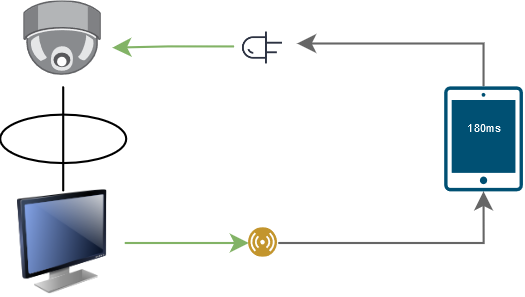
\includegraphics[scale = 0.75]{Figures/latency_tester.png}
    \caption{Equipo de medición de latencias conceptual}
    \label{fig:latency_tester}
\end{figure}

Para el desarrollo de este equipo de medición se han seleccionado como fundamentales una serie de componentes que serán descritos a continuación:

\begin{itemize}
    \item LED: será la fuente de estímulos primaria del equipo de mediciones, que este caso, serán luminosos. Se empleará esta tecnología debido principalmente a su relación entre bajo consumo energético, y alto poder luminiscente, unido a la bajísima latencia con la que son capaces de reaccionar.
    \item Fotosensor: pegado al monitor del sistema de vídeo, actuará como el receptor de los estímulos luminosos que capte la cámara de vídeo.
    \item Placa programable: encargada de coordinar al LED, el sensor y realizar los cálculos pertinentes para mostrar como salida la latencia que se produce en el sistema de vídeo.
    \item Conversor analógico digital: dado que nuestra placa seleccionada solo tiene pines GPIO digitales se precisa de este componente en forma de placa más pequeña para ampliar los pines originales y poder conectar con el fotosensor.
    \item Batería: que convertirá al equipo de medición en portátil, permitiendo así que sea transportable.
    \item Pantalla táctil: que tendrá por función el manejo del equipo de medición y el muestreo de las latencias medidas.
    \item Carcasa: que proteja y encapsule todos los componentes listados anteriormente.
\end{itemize}

Durante las etapas de gestación y propuesta de este mismo proyecto, se ha realizado un prototipo de sistema de medición en colaboración con GTD Defense \& Security SLU, utilizando un esquema intermedio al propuesto por Voysys y al que será final de este proyecto. Se ha llevado a cabo el desarrollo del prototipo a fin de estudiar previamente la viabilidad del proyecto antes de su realización y la redacción de este documento. Este prototipo, apenas funcional, resulta en una aproximación a ambas partes ya que cuenta con los elementos comunes ya descritos anteriormente y además es portátil, aunque dependiente de una fuente de energía externa para funcionar al no disponer de batería. Realiza cálculos y mediciones utilizando una placa Arduino Uno \cite{arduino} y además es capaz de mostrar una escueta salida de datos y mediciones a través de una pantalla digital en formato array. Ver Figura \ref{fig:prototipe}

\begin{figure}[H]
    \centering
    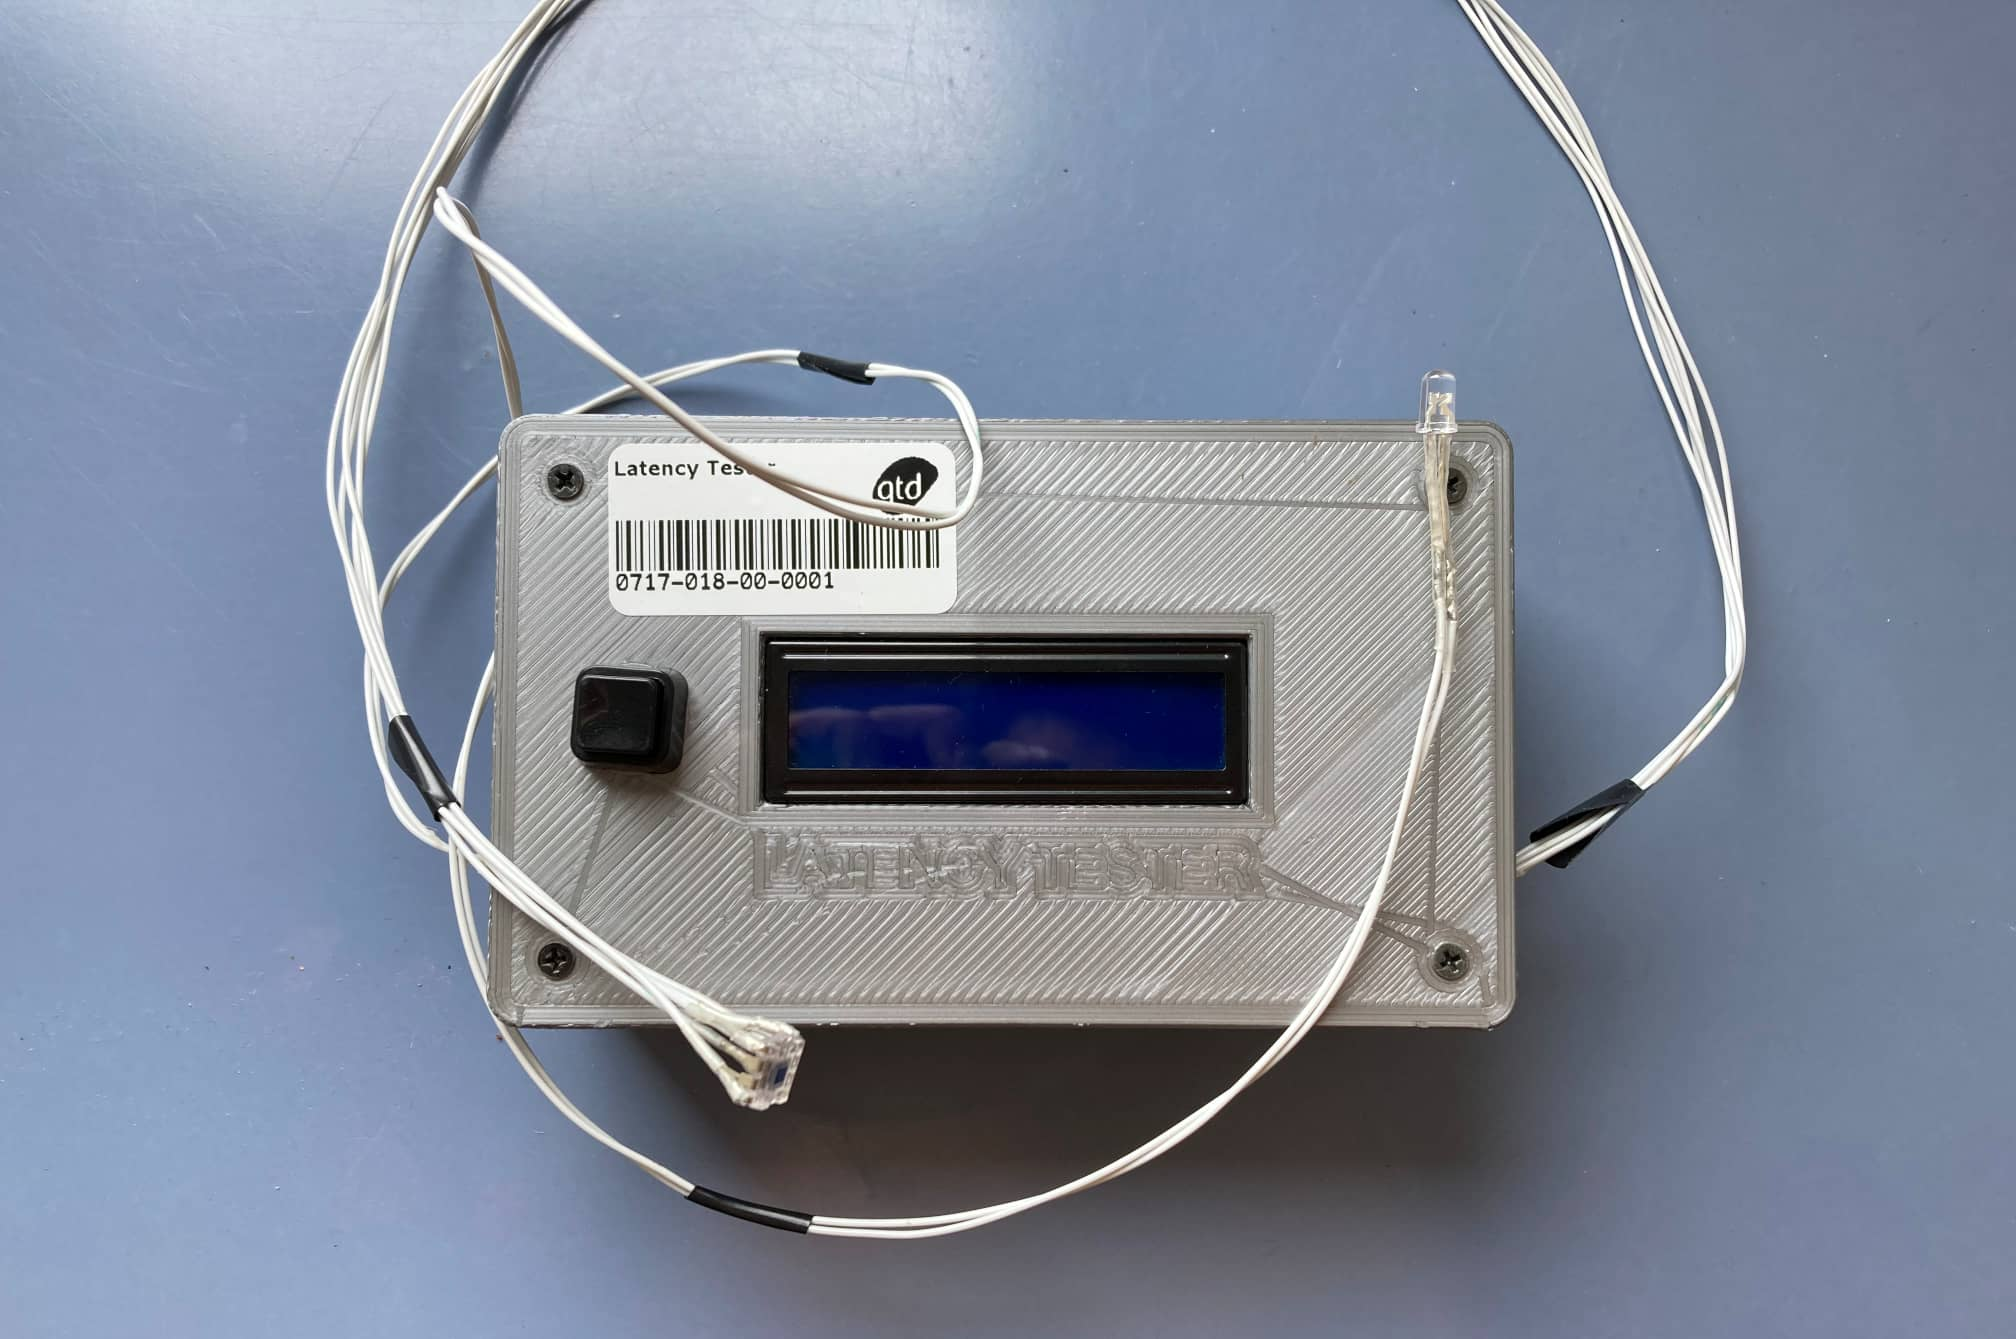
\includegraphics[scale = 0.075]{Figures/prototipo.jpg}
    \caption{Prototipo inicial de viabilidad de proyecto}
    \label{fig:prototipe}
\end{figure}

\subsection{Entorno del producto}

El producto nace bajo el paraguas de la optrónica para ser utilizado en entornos empresariales e industriales, a fin de poder medir los rendimientos de equipos de videovigilancia militares, pero lo cierto es que su aplicación puede extenderse a cualquier equipo de grabación de vídeos que lo requiera, y generalizarse su utilización al ámbito doméstico sin problemas.
Por ejemplo, dándonos una medición de cuánto tarda una imagen desde que es captada por la lente de nuestro teléfono, hasta que esta es proyectada en la pantalla del mismo, o cuánto retardo tienen una cámara ip o webcam al retransmitir a través de una red local o directamente en streaming a través de una conexión al exterior teniendo en cuenta procesados intermedios, latencias de la red, e incluso de tiempos de respuesta y refresco del monitor.

\section{Funciones}

La principal y única función de este equipo medidor de latencias es la de cuantificar el retardo de un sistema de videovigilancia tomando como punto inicial la toma de la imagen y como final, su retransmisión a través del monitor, mostrando este cálculo el equipo en su pantalla.
El dispositivo podrá así mismo graficar el retardo que tiene la entrada en ser procesada y mostrada con respecto a una línea temporal y además será capaz de funcionar en la mayor diversidad posible de entornos lumínicos y con la mayoría de cámaras y sistemas de videovigilancia conocidos, esto incluye algunas de las variedades de sistemas de visión nocturna previamente mostradas en este documento.

\section{Características del usuario}

El equipo de medición de latencias desarrollado está pensado para ser un dispositivo \textbf{sencillo}, que funcione en multitud de entornos sin necesidad de grandes adaptaciones o instalaciones costosas. 
Tendrá formas rectangulares, similar al prototipo de la figura \ref{fig:prototipe} y será \textbf{portátil}, para poder transportarlo de un lugar a otro con facilidad. Para ello estará equipado con una \textbf{batería}, que le permitirá funcionar sin conexión directa a la red eléctrica.
Vendrá equipado con una luz \textbf{LED} de bajo consumo y alta intensidad lumínica cuyo parpadeo actuará como estímulo de entrada a ser medido por el equipo. En el otro extremo del equipo de medición, existirá un \textbf{fotosensor} que instalará en el monitor del CCTV y que será el receptor de los impulsos emitidos por el LED. Ambos, LED y fotosensor, irán conectados al equipo por medio de cables.
Así mismo, el equipo dispondrá de una \textbf{pantalla táctil} que dará acceso a un \textbf{intuitivo} software de control para realizar las mediciones. Este software se cargará automáticamente al encender el dispositivo y tendrá un menú inicial con un botón para iniciar mediciones y un botón de configuración. Se dispondrá también de una función de calibración del sensor que permita adaptarlo a las condiciones lumínicas del entorno de medida, de forma que se facilite la obtención de resultados fiables.
Todo este software, será ejecutado sobre una \textbf{Raspberry Pi Model 3B}.

% TODO: Figura aquí con todos los componentes

\section{Restricciones generales}

Entre las posibles restricciones que se han encontrado a la hora de crear el equipo de medición de latencias podemos enumerar:

\begin{itemize}
    \item \textbf{Capacidad de medición en entornos muy luminoso}. Se tiene dependencia de un LED que puede variar en tamaño e intensidad, pero que en situaciones de mucha luz, se verá crispado para conseguir destacar en el ambiente. Se considera en este proyecto un ambiente muy luminoso cualquiera que parta de los 300 lúmenes, como puedan ser estancias con amplia iluminación natural o exposición solar directa. %TODO: realizar medidas y variar el número en consonancia
    \item \textbf{Capacidad de medición en sistemas de vídeo térmico}. Al tratarse de equipos que detectan y aumentan el contraste de las imágenes que desprenden calor, el LED deja de resultar útil en estos casos, siendo preciso idear un nuevo sistema para llevar a término las mediciones en estos sistemas.
    \item \textbf{Capacidad de la batería}. Factor limitante en tanto en cuando se depende de ella para el funcionamiento del dispositivo y establece cuanto tiempo podrá permanecer en funcionamiento el equipo de medición. A su vez, la restricción a la batería es impuesta por el coste de la misma, el peso que añada al dispositivo, que debe seguir siendo portátil, y el propio espacio disponible para ella dentro de la carcasa con el resto de componentes ensamblados.
    \item \textbf{Longitud de los cables del medidor}. Será una restricción debido a que no se podrán realizar mediciones en CCTV's que ya se encuentren instalados, ya que el LED y el fotosensor tienen únicamente un metro de separación entre ellos. Esto será debido a que en primera instancia, el diseño del dispositivo no contempla la latencia introducida por su propio cableado en el tiempo de encendido del LED y la recepción de las señales del sensor, lo cuál obliga a utilizar un cable de corta longitud, de un metro, para no añadir más variables a las mediciones.
    \item \textbf{Longitud de los cables de los CCTV's}. Se precisarán de los cables que se utilizarán en la instalación de los equipos para llevar a cabo las mediciones, ya que, dos cámaras conectadas al mismo monitor, pero con cables de longitud distinta, tendrán distinta latencia.
\end{itemize}

\subsection{Tecnologías empleadas}

Se llevará a cabo el desarrollo e implementación del software del equipo de medición de latencias utilizando las siguientes herramientas de programación que serán citadas y descritas a continuación:

\begin{itemize}
    \item Lenguaje de programación C++ \cite{c++}. En su estándar 2020, utilizando su compilador GNU g++, en su versión 11. Será el lenguaje elegido por preferencia personal del autor, y al ser un lenguaje más cercano al entorno hardware que a menudo proporciona un rendimiento de ejecución superior en todas las aplicaciones.
    \item Biblioteca de funciones standard de C++.
    \item Biblioteca de funciones boost \cite{boost}. En su versión 1.77, que proporcionan un extra de funcionalidad sobre la biblioteca standard de C++, permitiendo aprovechar desarrollos de algoritmos ya implementados y probados en lugar de desarrollarlos de cero para este proyecto.
    \item Qt framework \cite{qt}. En su versión 6, el cuál servirá para el desarrollo de la interfaz de usuario del equipo de medición y ayudar a elevar el nivel de la implementación gracias a la simplificación que provee para tareas que de otro modo serían muy tediosas. Incluye además el módulo Qt Virtual Keyboard para entrada táctil sin dependencias de teclados virtuales externos.
    \item Sistema de construcción qmake, incluido con Qt, que genera los ficheros Makefile a partir del archivo de proyecto (.pro) y gestiona automáticamente las dependencias, la invocación del preprocesador de meta-objetos (MOC), la compilación de formularios (.ui) y la generación de traducciones (.qm).
    \item GNU Make, herramienta de automatización de compilación que ejecuta los Makefile generados por qmake, resolviendo el grafo de dependencias entre ficheros fuente y objetos, y paralelizando la compilación cuando es posible.
    \item ARM GNU Toolchain (anteriormente Linaro), cadena de herramientas de compilación cruzada que permite generar binarios ejecutables para arquitectura ARM v8 (Raspberry Pi) desde un ordenador de desarrollo x86-64. Incluye los compiladores \texttt{aarch64-linux-gnu-gcc} y \texttt{aarch64-linux-gnu-g++}, el enlazador y las utilidades binarias asociadas.
    \item Se utilizarán algunas bibliotecas de funciones externas extraídas de internet para facilitar el desarrollo de ciertas funcionalidades. Algunas de ellas serán: QCustomPlot \cite{qtcustomplot}, para graficar los resultados de las mediciones, PiGpio \cite{pigpio} para facilitar el acceso a los pines GPIO de la Raspberry Pi, y rpi\_ads1115 para la lectura analógica del fotosensor a través del conversor analógico-digital ADS1115 mediante I2C.
    \item Doxygen, herramienta de generación automática de documentación a partir de los comentarios presentes en el código fuente C++. Produce documentación navegable en formato HTML con diagramas de clases, grafos de llamadas y relaciones de herencia, facilitando la comprensión y mantenimiento del proyecto.
    \item Graphviz (dot), motor de renderizado de grafos utilizado por Doxygen para generar diagramas de clases, colaboración y llamadas en formato SVG. Permite visualizar la arquitectura del software de forma automática a partir del análisis estático del código.
    \item Scripts de automatización Bash (Linux) y PowerShell (Windows) que unifican en un solo comando la compilación del proyecto en modo Release y la generación de la documentación Doxygen, simplificando el flujo de trabajo del desarrollador y la integración continua.
    \item AddressSanitizer (ASan), herramienta de detección de errores de memoria integrada en GCC y Clang. Se activa automáticamente en compilaciones Debug sobre Linux, y detecta en tiempo de ejecución fugas de memoria, desbordamientos de buffer y accesos a memoria liberada, abortando el proceso con un informe detallado del lugar exacto del error.
\end{itemize}

Respecto a la gestión de dependencias externas, se ha optado por la utilización de submódulos de Git para incorporar al repositorio del proyecto aquellas bibliotecas de terceros que se mantienen en repositorios externos. En concreto, la biblioteca rpi\_ads1115 se gestiona como un submódulo Git que referencia el repositorio original de su autor. Este enfoque permite mantener un vínculo directo con la fuente original, facilitar las actualizaciones futuras de la dependencia y mantener separado el código propio del código de terceros. La biblioteca QCustomPlot, por su parte, se incluye directamente en el repositorio al haber sido parcheada para garantizar su compatibilidad con Qt 6.

Tras la comparativa técnica realizada en \ref{hardware}, a continuación se mostrará otra tabla comparativa que, al final, acabará desembocando en la conclusión de por qué se ha elegido la Raspberry Pi Model 3B en lugar del Arduino Uno u otras posibles alternativas. Ver tabla \ref{tab:hardware2}.

\begin{table}[H]
\caption{Comparativa de placas programables II}
\label{tab:hardware2}
\begin{longtable}[c]{|c|c|}
\toprule 
\textbf{Arduino} & \textbf{Raspberry Pi}\tabularnewline
\midrule 
Parte de un ordenador, que ejecuta & Es un mini PC que puede ejecutar \tabularnewline
un único programa una y otra vez. & múltiples programas al mismo tiempo. \tabularnewline
\midrule 
Pensado para funcionar con & Complicado de hacer funcionar \tabularnewline
batería. & con batería. \tabularnewline
\midrule
Sus componentes y sensores & Requiere instalar bibliotecas \tabularnewline
funcionan de manera & y software para interactuar con sensores \tabularnewline
integrada. & y otros componentes. \tabularnewline
\midrule
Es barato. & Es caro en relación a Arduino. \tabularnewline
\midrule 
Requiere hardware externo & Se conecta fácilmente a internet \tabularnewline
para conectarse a internet & con su puerto RJ-45 o WiFi por USB. \tabularnewline
y hay que programarlo para ello. & \tabularnewline
\midrule 
Puede venir con almacenamiento & No tiene almacenamiento, pero \tabularnewline
integrado. & puede usar su ranura \tabularnewline
& micro SD para ello. \tabularnewline
\midrule 
Es un dispositivo & Se debe apagar correctamente \tabularnewline
plug \& play. & para que no haya riesgo de \tabularnewline
& corrupción de archivos. \tabularnewline
\midrule 
Solo utiliza Arduino y & Se recomienda Python \tabularnewline
y C/C++. & pero puede usar C, C++ y Ruby. \tabularnewline
\midrule
Tiene pines i/o & No tiene pines i/o \tabularnewline
analógicos. & analógicos. \tabularnewline
\bottomrule
\end{longtable}
\end{table}

Se ha decidido utilizar finalmente la Raspberry Pi 3 Model B debido a su mayor versatilidad con respecto al Arduino, ya que a la hora de implementar el software, Arduino no es compatible con pantallas táctiles de alta resolución y profundidad de color, dando lugar así a una interfaz de usuario menos amigable.
Se ha decidido descartar de esta comparativa arquitecturas de procesador más complejas, como x86-64 \cite{ye2006performance}, por los siguientes motivos:

\begin{enumerate}
    \item Aumento significativo del coste del SBC.
    \item Mayor tamaño físico de las placas.
    \item Necesidad de mayor disipación de calor.
    \item Gran aumento del consumo energético, en detrimento de la duración de la batería.
\end{enumerate}

Se utilizarán estas herramientas ajustando sus parámetros para ser compatibles con procesadores de arquitectura ARM que es la que posee la Raspberry Pi 3 que será utilizada como SBC para el equipo. El modelo concreto cuenta con las siguientes especificaciones:

\begin{itemize}
    \item Raspberry Pi 3 Model B.
    \item Chipset Broadcon de 64 bits y 4 núcleos ARM.
    \item Memoria RAM de 1GB.
    \item Coprocesador multimedia de doble núcleo.
    \item Pines digitales de entrada y salida.
    \item Protocolo I2C\cite{i2c}.
\end{itemize}

A estas herramientas habrá que añadir una base de trabajo en forma de sistema operativo, que para el caso, será Raspbian, versión Lite ahora llamada Raspi OS, distribución linux basada en Debian, para Raspberry Pi y que por antonomasia, es referente en buen funcionamiento y estabilidad. Este sistema irá personalizado para ofrecer una experiencia únicamente centrada en la medición de latencias.
Sobre Raspi Os se ejecutará un script a la inicialización del sistema que será el encargado de lanzar la aplicación automáticamente.

Se desarrollará todo el proyecto sobre el IDE Qt Creator versión 16, el cual da soporte a todos los elementos de programación anteriormente mencionados, con gran capacidad de abstracción, y en un entorno gráfico amigable. Además provee de herramientas de trabajo compatibles con sistemas embebidos que facilitarán la tarea de generar versiones del software para un dispositivo no X86-64 como es la Raspberry Pi.

De cara al control de versiones, se propone la utilización de un repositorio privado durante el desarrollo del producto, alojado en Github y controlado con Git y Qt Creator.

Para facilitar todo el desarrollo, en un entorno controlado, se pretendía, en un inicio, utilizar una máquina virtual con Raspi Os la cual correrá sobre VirtualBox \cite{virtualbox}. Se encuentra el impedimento de que no existe una versión de Raspo Os, suficientemente actualizada para la ejecución del proyecto en arquitectura x86-64. A esto hay que añadir, la incompatibilidad de las bibliotecas de funciones, que compiladas en arquitectura x86-64, no resultarían útiles a la hora de portar el proyecto software a la placa programable final y además, en este caso al ser un proyecto que trabaja directamente sobre el hardware de la placa, en este caso, los pines GPIO, y la pantalla táctil, imposibilitaría la necesidad de ir haciendo pruebas directamente sobre la máquina virtual, requiriendo del hardware real para poder testar todo el código escrito relacionado a estos respectos.
Se propone en este caso, trabajar directamente sobre arquitectura x86, sin necesidad de virtualizar nada, con el objetivo de aumentar el rendimiento de trabajo, acortar tiempos de espera y simplificar la sincronización del hardware arm con la máquina x86, eliminando la capa hipervisora que de otra forma correría funcionando sobre el ordenador de desarrollo.
A este respecto se ha utilizado una compilación cruzada a través de un compilador para arm que trabaja directamente sobre las bibliotecas de funciones extraídas de la Raspberry Pi, ya precompiladas en ARM. Todos estos ficheros se extraen y copian a la máquina x86 la cuál servirá de plataforma para la compilación cruzada y el despliegue del proyecto posterior en la placa programable.
La interconexión para compartir las bibliotecas de funciones entre la Raspberry Pi y el pc x86, se realizarás a través de conexión SSH \cite{ssh}, mediante la herramienta rsync\cite{rsync}. A su vez, a la hora de desplegar la aplicación ya compilada desde la máquina x86, se volverá a recurrir al protocolo SSH\cite{ssh}.
En el caso, para compilar el proyecto, se utilizará el ARM GNU Toolchain, antiguamente conocido como Linaro. La configuración de la toolchain necesaria para compilar desde un ordenador x64 a ARM v8 se explicará más adelante en este documento, pero se adelanta que funcionará utilizando el compilador gcc y g++ en sus respectivas ediciones ARM.
Una toolchain o cadena de herramientas, que sería su traducción literal, en informática se refiere a un conjunto de programas que utilizados en cadena, es decir, enlazando la salida de uno con la entrada de otro, ayudan en la generación de un producto software.

Una consideración muy a tener en cuenta durante el análisis de la placa a utilizar, es que la Raspberry frente a Arduino, no tiene pines de entrada/salida analógicos, con lo cuál no podrá ser utilizada inicialmente para hacer lecturas del sensor de luz OPT101, que es, en este caso, el elegido para el proyecto frente al resto de sus competidores de tipo foto resistivo, los cuáles tienen un tiempo de respuesta superior y no son tan apropiados para hacer mediciones de latencias que deben ser "instantáneas". Es este y no otro, el motivo por el cual ha sido elegido candidato para la realización de este proyecto. Para salvar este escoyo, que no se tuvo en cuenta durante el análisis inicial del proyecto se ha recurrido a I2C\cite{i2c}, una interfaz de intercomunicación de circuitos que tiene integrada la Raspberry Pi en sus pines GPIO y que es posible activar desde la bios de configuración de la misma. Será, utilizando esta interfaz, la biblioteca PiGpio\cite{pigpio}, y un conversor de señal analógico digital modelo ADS1115.

\chapter{Desarrollo del proyecto}

El medidor de latencias para sistemas de videovigilancia, es un dispositivo, que de manera sencilla, a través de la emisión y captación de un impulso lumínico, realiza los cálculos necesarios para averiguar el tiempo existente que necesita un dispositivo de vídeo desde que capta una imagen hasta que la proyecta en un monitor.
Se detallarán en este capítulo, las fases de su ciclo comercial, como funciona, que características y apariencia tendrán su sistema software, que problemas es capaz de resolver y como está programado.

\section{Modelo de ciclo de vida}

Se describe a continuación cuales son las posibilidades del producto a lo largo de su vida útil más allá del alcance de este proyecto. Como se pretende comercializar el producto, se proporciona a continuación un modelo de ciclo de vida con la planificación estratificada de las expectativas actuales al respecto.

\begin{itemize}
    \item \textbf{Desarrollo del producto}: Se comienza el proyecto en esta fase, que es la que ocupa la redacción de este documento. Inicialmente, se concibe la idea como un proyecto con potencial, que no tiene competencia en el mercado y en el que hay que hacer una inversión inicial para su desarrollo. Se asume aquí que el prototipo del proyecto tal como se está desarrollando cumple unos mínimos requisitos de funcionalidad y que además es viable en cuanto a coste económico y tiempo. Se desarrolla el medidor de latencia teniendo en cuenta su posible actualización posterior en función de su continuidad o las necesidades.
    
    \item \textbf{Crecimiento y primera gran actualización del producto}: Se proponen cambios de calado para reducir los costes de producción del prototipo, facilitar su transporte reduciendo su peso, y reducir su consumo energético como compromiso para aumentar su autonomía. Para ello, se propone el desarrollo de un sistema operativo propio que reduzca y optimice el coste de recursos software necesarios para el funcionamiento del dispositivo. En conjunción con este sistema operativo, será necesario establecer un sistema de compilación cruzada que permitirá generar y cargar versiones del software del medidor de latencias mucho más rápido que anteriormente y facilitará ampliamente su despliegue.
    
    \item \textbf{Madurez y adaptación a nuevos requisitos}: Se actualizará el producto con una nueva versión del software para cumplir con los nuevos requisitos que se puedan integrar en el medidor y se realizará también el cambio de la placa Raspberry Pi 3 Model B por una Pi Zero 2 W (susceptible de cambio si apareciese un nuevo modelo), mucho más pequeña, eficiente y barata.
    
    \item \textbf{Declive del producto}: Se irá abandonando paulatinamente el desarrollo del producto una vez alcanzado el final del desarrollo y garantías de su etapa de madurez.
\end{itemize}

En cuanto al producto software, se seguirá un modelo de ciclo de vida tradicional, en cascada, tal como puede apreciarse en el diagrama de \ref{fig:calendar}{Gantt}.

\begin{figure}[H]
    \centering
    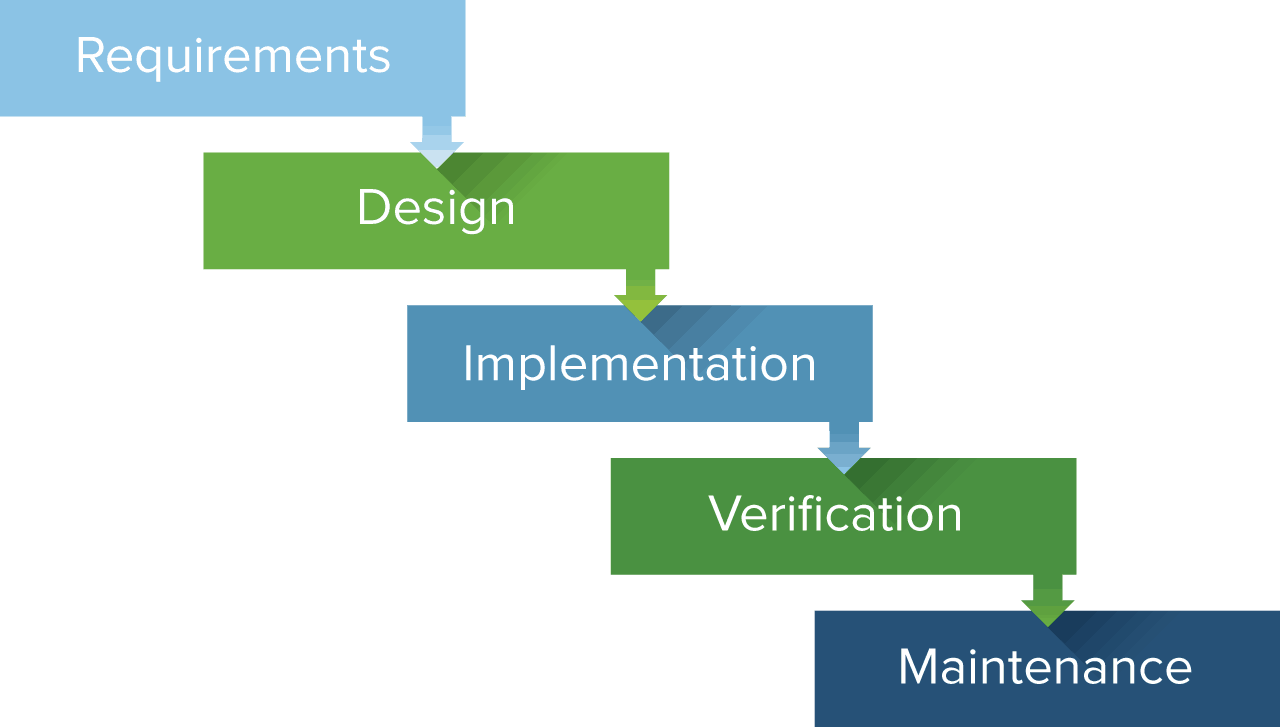
\includegraphics[scale = 0.25]{Figures/cascade_life_cycle.png}
    \caption{Modelo de ciclo de vida en cascada. Fuente: \cite{waterfall_methodology}}
    \label{fig:waterfall_lifecycle}
\end{figure}

\section{Requisitos}

\subsection{Funcionales}

% En este apartado se describirá los servicios que provee y la forma en el que el dispositivo medidor de latencias responderá a las entradas del sistema y los eventos externos.

\begin{enumerate}
    \renewcommand{\theenumi}{R.F.\arabic{enumi}}
    \renewcommand{\theenumii}{\theenumi.\arabic{enumii}}
    \renewcommand{\theenumiii}{\theenumii.\arabic{enumiii}}
    \item Como usuario se desea que su aspecto físico, sea el de una caja plastica PLA rectangular, impresa en 3D con unas dimensiones de (insertar dimensiones reales aquí), que incorpore una pantalla táctil en su frontal y un conmutador de encendido en alguno de sus laterales.
    \item Como usuario se solicita que en la carcasa, se disponga también de tres aberturas funcionales. 
    \begin{enumerate}
        \item La primera, será utilizada para el puerto de carga de la batería del medidor de latencia.
        \item Otras serán para la salida de los cables que conectan con el led emisor.
        \item La tercera será para el sensor fotosensible que recibirá los estímulos del led en el monitor.
    \end{enumerate}
    \item Como usuario se desea que dentro de la carcasa, bajo la pantalla, se encontrarán las baterías, y una placa Raspberry Pi Model 3B. 
    \item Como usuario se quiere que esta placa vaya anclada a la carcasa, con los cables del led y el sensor soldados en los pines de entrada/salida correspondientes. 
    \item Como usuario se decide que la placa irá equipada con una memoria secundaria en forma de tarjeta micro SD de alta capacidad, mínimo 8GB y velocidad, mínimo 10mb/s de lectura secuencial. 
    \item Como usuario se quiere desarrollar el Medidor de latencia como producto físico y tangible, que a su vez incorpora un producto software. 
    \item Como usuario se quiere que dicho producto software sea sencillo y cuente con: 
\begin{enumerate}
    \item Un menú inicial. 
    \item Una pantalla de configuración paramétrica. 
    \item Una pantalla para la medición.
    \label{rf73}
    \item Una pantalla de ayuda.
\end{enumerate}
    \item Como usuario, se especifica que el medidor de latencias arrancará automáticamente el software de mediciones tras encenderse.
    \item Como usuario se quiere conocer el estado de carga de la batería en la esquina superior de la pantalla en todo momento.
    \item Como usuario se interactuará con el dispositivo únicamente a través de la pantalla táctil.
    \item Como usuario se desea que se desencadenen respuesta a las entradas táctiles únicamente en los botones y cajas contenedoras de datos habilitadas para ello (checkboxes, comboboxes, botones).
    \item Como usuario se quiere que la pantalla principal del dispositivo permita acceder a la pantalla de configuración del dispositivo, la de mediciones, al histórico de mediciones y la pantalla de ayuda.
    \item Como usuario se especifica que en toda pantalla que no sea la principal, existirá un botón de retroceso a la pantalla anterior.
    \item Como usuario se quiere que desde la pantalla de configuración se puedan cambiar: 
    \begin{enumerate}
        \item Opciones de accesibilidad.
            \begin{enumerate}
                \item Aumento del tamaño de la fuente del texto.
                \label{rf1411}
                \item Modo daltónicos.
                \label{rf1412}
                \item Modo noche.
                \label{rf1413}
            \end{enumerate}
        \item El idioma de los textos entre:
        \label{rf14}
        \begin{enumerate}
            \item Español.
            \item Inglés.
            \item Polaco.
        \end{enumerate}
        \item Consultar la información de versión y licencia.
    \end{enumerate}
    \item Como usuario, se quiere que la configuración se guarde entre reinicios.
    \label{rf15}
    \item Como usuario se quiere que el lenguaje por defecto del software sea español.
    \label{rf16}
    \item Como usuario se desea que desde la pantalla de mediciones se puedan visualizar los resultados de las mediciones de latencia en forma de gráfico bidimensional cíclico, en base al tiempo entre mediciones especificado, en tiempo real mientras se van realizando. 
    \item Como usuario se quiere mostrar numéricamente en ms's la latencia del sistema medido en tiempo real mientras se realiza la medición.
    \item Como usuario se quiere comenzar la medición pulsando un botón dentro de la pantalla de mediciones.
    \item Como usuario se quiere poder pausar la medición pulsando el mismo botón de inicio dentro de la pantalla de mediciones.
    \item Como usuario se especifica que se podrá detener la medición con un botón situado a la derecha del de iniciar medición.
    \item Como usuario se quiere poder especificar la duración máxima de una medición en minutos y segundos previa a su realización.
    \item Como usuario se especifica que debe saberse en todo momento el tiempo de la medición restante para su finalización.
    \item Como usuario se requiere que este botón esté bloqueado mientras no exista una medición en curso.
    \item Como usuario se desea tener la posibilidad de cambiar la frecuencia de las mediciones directamente desde la pantalla de mediciones.
    \item Como usuario se especifica que al volver a la pantalla inicial, se ofrecerá guardar la medición en el registro.
    \item Como usuario se desea que al seleccionar que se quiere guardar la medición, permitirá darle un nombre.
    \item Como usuario se quiere que las mediciones se guarden en un registro de mediciones en formato JSON.
    \label{rf28}
    \item Como usuario se desea que cada medición realizada esté identificada por un nombre.
    \label{rf29}
    \item Como usuario se especifica que quedará registrada la fecha en que se realizó cada medición.
    \label{rf30}
    \item Como usuario se quiere tener almacenado de cada medición:
    \begin{enumerate}
        \item Nombre que la identifique
        \item Fecha en que fue realizada en formato \textit{hh:mm dd/mm/yyyy}.
        \item El tiempo en ms's que se ha utilizado entre mediciones.
        \item Las latencia calculada para cada medición.
    \end{enumerate}
    \item Como usuario se quiere que el registro se almacene por orden cronológico.
    \item Como usuario se desea que cada medición se muestre por su nombre en el registro.
    \item Como usuario se especifica que al acceder a una medición registrada, se mostrará su latencia media en ms's.
    \label{rf34}
    \item Como usuario se quiere que el registro permita volver a ver el gráfico de una medición pulsando un botón en la pantalla del registro de la medición.
    \label{rf35}
    \item Como usuario se quiere mostrar un manual de instrucciones dentro de la pantalla ayuda, en forma de texto.
    \item Como usuario se desea que el dispositivo medidor se apague tras treinta minutos sin actividad.
    \label{rf37}
    \item Como usuario se especifica, que el medidor de latencias deberá reducir el brillo de la pantalla al mínimo tras quince minutos de actividad.
    \label{rf38}
    \item Como usuario se requiere que la calibración del medidor de latencias se ajuste al entorno en el que se realice la medición.
    \label{rf39}
    \item Como usuario se especifica que el modo nocturno y el modo daltónicos son funcionalidades ortogonales e independientes, pudiendo estar ambos activos simultáneamente. En caso de activarse ambos, el modo daltónicos tendrá prioridad sobre los colores de los botones y widgets, mientras que el modo nocturno mantendrá el fondo oscuro de la interfaz.
    \label{rf40}
\end{enumerate}

\subsection{Requisitos del hardware}

Se presentan a continuación los \textbf{requisitos mínimos} hardware para desarrollar el medidor de latencias, estos corresponden a su desarrollo con una Raspberry Pi Zero 2w:

\begin{enumerate}
\renewcommand{\theenumi}{R.H.M.\arabic{enumi}}
\renewcommand{\theenumii}{\theenumi.\arabic{enumii}}
\renewcommand{\theenumiii}{\theenumii.\arabic{enumiii}}
    \item Procesador: 1GHz quad-core 64-bit Arm Cortex-A53 CPU.
    \item Memoria ram: 512MB SDRAM.
    \item Capacidad de disco: microSD card slot y tarjeta micro sd HC de 8GB.
    \item Pines GPIO: HAT-compatible 40-pin header footprint (unpopulated).
    \item Energía: Micro USB power
    \item Batería: $\geq 1200$ mAh de capacidad.
    \item Pantalla: Tactil resistiva de 3,5'' con resolución 480 x 320 píxeles con conexión por pines GPIO.
    \item Diodo Led de alta luminancia.
    \item Fotosensor de alta sensibilidad.
    \item Carcasa rectangular fabricada en PLA de alto x largo x ancho.
\end{enumerate}

Para una mayor fluidez de funcionamiento y versatilidad se proponen \textbf{requisitos recomendados}: 

\begin{enumerate}
\renewcommand{\theenumi}{R.H.R.\arabic{enumi}}
\renewcommand{\theenumii}{\theenumi.\arabic{enumii}}
\renewcommand{\theenumiii}{\theenumii.\arabic{enumiii}}
    \item Procesador: 1,4GHz quad-core 64-bit Arm Cortex-A53 CPU.
    \item Memoria ram: 1GB SDRAM.
    \item Batería: $\geq 3000$ mAh de capacidad.
    \item Pantalla: Tactil capacitiva multipunto de 7'' con resolución 800 x 480 pixeles y conexión SPI.
\end{enumerate}

Este medidor de latencia se utilizará un modelo más común de Raspberry, la Raspberry Pi 3 Model B, el cual sobrepasa todos los requisitos mínimos establecidos para el sistema y además añade la posibilidad de utilizar pantallas con conexión SPI de mayor tamaño, que no ocupan los pines GPIO, y tienen superficie táctil multipunto y capacitiva en lugar de resistivas.

\subsection{Interfaz}

\begin{enumerate}
    \renewcommand{\theenumi}{R.I.\arabic{enumi}}
    \renewcommand{\theenumii}{\theenumi.\arabic{enumii}}
    \renewcommand{\theenumiii}{\theenumii.\arabic{enumiii}}
    \item Como usuario se quiere que la interfaz de usuario por defecto se muestre apaisada y no en vertical.
    \item Como usuario se quiere que la interfaz disponga de un modo claro (por defecto) y un modo nocturno activable desde ajustes.
    \item Como usuario se especifica que se quiere una fuente clara y legible con buen contraste sobre el fondo.
    \label{ri3}
    \item Como usuario se desea que el tamaño de la fuente mínimo sea 9 y el máximo 15.
    \label{ri4}
    \item Como usuario se desea que la fuente del texto sea de color blanco y en \textbf{negrita} en los botones para garantizar la legibilidad.
    \label{ri5}
    \item Como usuario se requiere que todas las pantallas tengan en el margen superior un marco a modo de barra de menú.
    \item Como usuario se pretende que en dicho marco se muestre en la zona central la hora de sistema y la fecha.
    \item Como usuario se quiere que en el marco superior en la esquina derecha se muestre el estado actual de carga de la batería.
    \begin{enumerate}
        \item Este estado actual debe mostrar gráficamente si se está cargando o descargando.
        \item Se tendrá en cuenta la posibilidad de mostrar porcentualmente la carga actual de la batería.
    \end{enumerate}
    \item Como usuario se especifica que en el borde superior izquierdo deberá haber disponible un botón de retroceso.
    \item Como usuario se quiere que este botón de retroceso tenga forma de flecha.
    \item Como usuario se especifica que el botón de retroceso únicamente será funcional en pantallas que no sean la principal y mientras no se esté realizando una medición o calibración.
    \item Como usuario se desea que todos los botones sean rectangulares con los bordes redondeados y un fondo semi-transparente distinguible del fondo de la pantalla.
    \item Como usuario se especifica que los botones de la pantalla de mediciones (Calibrar, Comenzar, Detener) deberán tener un tamaño suficiente para ser legibles y operables en pantalla táctil.
    \item Como usuario se requiere que el botón ``Comenzar'' esté situado en la zona derecha de la pantalla de mediciones, debajo del botón ``Calibrar''.
    \item Como usuario se quiere que el botón ``Detener'' se encuentre debajo de ``Comenzar'' y permanezca desactivado por defecto hasta que se inicie una calibración o medición.
    \item Como usuario se especifica que durante una calibración o medición en curso, todos los controles de la pantalla de mediciones se desactivarán excepto el botón ``Detener''.
    \item Como usuario se desea que durante una operación en curso, el botón correspondiente parpadee alternando colores como indicador de actividad.
    \item Como usuario se requiere que al finalizar una operación con éxito, el botón parpadee brevemente en verde, y en rojo si hubo un error.
    \item Como usuario se requiere que existan sliders para configurar el intervalo entre mediciones y la duración total antes de iniciar la medición.
    \item Como usuario se especifica que la interfaz del medidor de latencias cumplirá con el estándar WCAG 2.0 level AA \cite{wcag}.
    \item Como usuario se especifica que la interfaz del medidor de latencias cumplirá con el estándar WCAG 2.1 \cite{wcag}.
    \item Como usuario se especifica que al activar simultáneamente el modo nocturno y el modo daltónicos, la interfaz presentará el fondo oscuro del modo nocturno junto con los colores de alto contraste del modo daltónicos en los botones y widgets interactivos. Los controles como sliders, checkboxes y comboboxes mantendrán la apariencia del modo nocturno, mientras que los botones de acción y el botón de retroceso adoptarán los colores del modo daltónicos.
    \item Como usuario se requiere que todos los sliders de la interfaz muestren en su etiqueta asociada el valor numérico actual junto con la unidad que representan, actualizándose en tiempo real al desplazar el control.
\end{enumerate}

\subsection{No funcionales}

\begin{enumerate}
    \renewcommand{\theenumi}{R.N.F.\arabic{enumi}}
    \renewcommand{\theenumii}{\theenumi.\arabic{enumii}}
    \renewcommand{\theenumiii}{\theenumii.\arabic{enumiii}}
    \item El sistema ha de ser fácil de operar, con formas y colores contrastados que permitan la legibilidad de las fuentes en todo momento, incluidas aquellas personas con problemas de visión como daltonismo, astigmatismo o presbicia.
    \label{rnf1}
    \item El sistema de medición de latencias ha de arrancar automáticamente una vez iniciado el dispositivo y ha de ser el único software que sea posible operar desde el mismo.
    \item El sistema de medición de latencias tiene que poder operar con solvencia con un máximo de 512MB de memoria RAM.
    \item El led utilizado en el sistema de medición de latencias debe ser capaz de ofrecer luminancia suficiente para ser fácilmente detectado en un ambiente de iluminación artificial media y controlada.
    \label{rnf4}
    \item El sistema de medición de latencias no estará concebido para realizar mediciones de campo en un entorno abierto de alta luminancia natural, sino en un laboratorio en condiciones controladas.
    \label{rnf5}
    \item El sistema de medición de latencias en su versión de desarrollo actual, no garantiza su correcto funcionamiento para mediciones de otro tipo de cámaras que no sean de TV. Se incluyen en este grupo, cámaras de visión nocturna, y térmicas.
    \label{rnf6}
    \item El sistema de medición de latencias necesitará en su versión actual de un soporte, o adhesivo, no incluidos, para la sujeción y fijación tanto del diodo led a la lente de la cámara, como del sensor fotolumínico al monitor.
    \item La batería del sistema medidor de latencias tendrá una duración estimada de al menos dos horas.
    \item La capacidad de memoria del medidor de latencias permitirá almacenar cientos de miles de mediciones sin ningún compromiso de capacidad.
    \item El SOC de la placa integrada en el medidor de latencias llevará incorporado un disipador de calor pasivo de cara a minimizar problemas derivados de un uso extensivo del mismo o su utilización en entornos con temperaturas extremas $(\geq \text{40ºC})$.
\end{enumerate}

\section{Análisis del sistema}

\subsection{Casos de uso}

% Esto es magia negra para crear listas de objetos en una tabla
\newcommand{\tabitem}{~~\llap{\textbullet}~~}
% Y esto para listas enumeradas
\newcounter{rownumbers}
\newcommand\rownumber{E.\stepcounter{rownumbers}\arabic{rownumbers}.}

\newcounter{steps}
\newcommand\step{\stepcounter{steps}\arabic{steps}.}

\newcounter{substeps}
\newcommand\substep{\arabic{steps}.\stepcounter{substeps}\arabic{substeps}.}

\begin{longtable}{|l|p{10cm}|}
\caption{C.U.1 Realizar medición} \\
\hline
C.U.1                     & Realizar medición\\ \hline \label{cu1}
Versión                   & 1.0 \\ \hline
Dependencias              & \tabitem \hyperref[rnf4]{R.N.F.4} \\ 
                          & \tabitem \hyperref[rnf5]{R.N.F.5} \\
                          & \tabitem \hyperref[rnf6]{R.N.F.6} \\\hline
Precondición              & El medidor de latencias deberá tener memoria \\ 
                          & suficiente para guardar la medición.\\ \hline
Descripción               & El sistema deberá comportarse como se describe \\ 
                          & en el siguiente caso de uso cuando \textit{el usuario del} \\ 
                          & \textit{medidor de latencias solicite realizar una medición}.\\ \hline
Secuencia normal          & \step El usuario solicita al sistema comenzar el proceso \\ 
de pasos                  & de medición de latencias de una cámara. \\
                          & \step El sistema pasa a la pantalla de realización de mediciones. \\
                          & \step El usuario elige la duración de la medición. \\
                          & \step El sistema guarda la duración de la medición. \\
                          & \step El usuario comienza la medición. \label{ex1} \\
                          & \step El sistema comienza a mostrar datos de las mediciones \\ 
                          & que va tomando. \\
                          & \substep El usuario puede variar el tiempo entre mediciones \\
                          & durante la medición. \\
                          & \substep El sistema cambiará el tiempo entre impulsos \\ 
                          & durante la medición. \\
                          & \step El tiempo configurado de la medición concluye. \\
                          & \step El sistema termina la medición, deja de mostrar \\
                          & datos y solicita un nombre para guardar la medición realizada. \label{paso8} \\ 
                          & \step El usuario introduce un nombre para la medición y pulsa guardar. \label{ex2} \\
                          & \step El sistema guarda la medición en el registro \\
                          & y sigue mostrando los datos de la medición tomada. \\ \hline
Postcondición             & El usuario puede ver los resultados finales de la \\
                          & medición y el sistema ha registrado la medición. \\ \hline
Excepciones               & \tabitem \hyperref[ex1]{Paso 4}. Si el usuario pulsa el botón de detener medición. \\
                          & \hspace{0.5cm} \rownumber El sistema continua en el \hyperref[paso8]{paso 8}. \\
                          & \tabitem \hyperref[ex2]{Paso 9}. El sistema no tiene memoria suficiente para \\ 
                          & almacenar la medición. \\
                          & \hspace{0.5cm} \rownumber El sistema avisa al usuario de que no \\ 
                          & tiene suficiente espacio de almacenamiento y \\ 
                          & recomienda borrar mediciones del registro o ampliar \\
                          & el almacenamiento. \\ \hline
Comentarios               & El número máximo de mediciones a guardar dependerá \\
                          & del almacenamiento disponible en la tarjeta sd y de \\
                          & la longitud de las mismas. El tiempo máximo de una \\
                          & medición será de 60 minutos. \\ \hline

\end{longtable}

\setcounter{rownumbers}{0}
\setcounter{steps}{0}
\setcounter{substeps}{0}

\begin{table}[H]
\caption{C.U.2 Consultar ayuda}
\begin{tabular}{|l|l|}
\hline
C.U.2                     & Consultar ayuda\\ \hline \label{cu2}
Versión                   & 1.0 \\ \hline
Dependencias              & \tabitem \hyperref[rnf1]{R.N.F.1} \\\hline
Precondición              & El medidor de latencias deberá tener memoria \\ 
                          & suficiente para guardar la medición.\\ \hline
Descripción               & El sistema tendrá una copia interna \\
                          & del manual de usuario para cuando el \\ 
                          & usuario no sepa como continuar.\\ \hline
Secuencia normal          & \step El usuario solicita al sistema \\
de pasos                  & consultar la ayuda del sistema. \\
                          & \step El sistema cambia a la pantalla de ayuda. \\
                          & \step El usuario elige ayuda sobre como realizar mediciones. \label{step3} \\
                          & \step El sistema muestra la sección del \\ 
                          & manual de usuario referente a la \\
                          & realización de mediciones. \\ \hline
Postcondición             & El sistema muestra las instrucciones de como \\
                          & operar con cada apartado del medidor de latencias. \\ \hline
Excepciones               & \tabitem \hyperref[step3]{Paso 3}. Si el usuario elige otro apartado \\
                          & sobre el que consultar la ayuda. \\
                          & \rownumber El sistema muestra la sección del manual \\
                          & referente a la información que se quiera consultar. \\ \hline
Comentarios               & El sistema incluirá una copia en texto del manual \\
                          & de usuario dentro de la sección ayuda. \\ \hline
\end{tabular}
\end{table}

\setcounter{rownumbers}{0}
\setcounter{steps}{0}
\setcounter{substeps}{0}

\begin{table}[H]
\caption{C.U.3 Configurar idioma}
\begin{tabular}{|l|l|}
\hline
C.U.3                     & Configurar idioma \\ \hline \label{cu3}
Versión                   & 1.0 \\ \hline
Dependencias              & \tabitem \hyperref[rf14]{R.F.14} \\
                          & \tabitem \hyperref[rf15]{R.F.15} \\
                          & \tabitem \hyperref[rf16]{R.F.16} \\\hline
Precondición              & El sistema inicia por primera vez en español. \\ \hline
Descripción               & El sistema permitirá el cambio del \\
                          & idioma en que se muestran los textos \\
                          & en pantalla por uno de los incluidos. \\ \hline
Secuencia normal          & \step El usuario entra en la configuración. \\
                          & \step El sistema muestra las opciones \\
                          & de configuración.\label{p2} \\
                          & \step El usuario selecciona la \\
                          & opción de cambio de idioma. \\
                          & \step El sistema muestra los idiomas \\
                          & disponibles. \label{p4} \\
                          & \step El usuario selecciona el \\
                          & idioma inglés y aplica los cambios. \label{p5} \\
                          & \step El sistema cambia el idioma \\
                          & de todos los textos a inglés. \\ \hline
Postcondición             & Los textos de todo el sistema quedan \\
                          & cambiados a inglés.\\ \hline
Excepciones               & \tabitem \hyperref[p5]{Paso 5}. Si el usuario elige otro idioma \\ 
                          & y aplica los cambios. \\
                          & \rownumber El sistema cambia el idioma \\
                          & de todos los textos al del idioma \\
                          & seleccionado. \\
                          & \tabitem \hyperref[p2]{Paso 2} - \hyperref[p4]{Paso 4}. Si el usuario pulsa el \\ 
                          & botón de retroceso: \\
                          & \rownumber Podrá ir retrocediendo pantallas \\
                          & una a una hasta llegar a la \\ 
                          & pantalla de inicio. \\ \hline
Comentarios               & Se tendrán disponible en el sistemas \\
                          & los lenguajes español, inglés y polaco. \\ \hline
\end{tabular}
\end{table}

\setcounter{rownumbers}{0}
\setcounter{steps}{0}
\setcounter{substeps}{0}

\begin{table}[H]
\caption{C.U.4 Activar modo daltónicos}
\begin{tabular}{|l|l|}
\hline
C.U.4                     & Activar modo daltónicos \\ \hline \label{cu4}
Versión                   & 1.0 \\ \hline
Dependencias              & \tabitem \hyperref[rf1412]{R.F.14.1.1} \\\hline
Precondición              & El sistema incluye un modo de corrección \\ 
                          & de color para facilitar su manejo a \\
                          & personas con daltonismo. \\ \hline
Descripción               & El sistema permitirá el cambio del \\
                          & idioma en que se muestran los textos \\
                          & en pantalla por uno de los incluidos. \\ \hline
Secuencia normal          & \step El usuario entra en la configuración. \\
                          & \step El sistema muestra las opciones \\
                          & de configuración. \label{pa2} \\
                          & \step El usuario selecciona las \\
                          & opciones de accesibilidad. \\
                          & \step El sistema muestra las opciones \\ 
                          & disponibles. \label{pa4} \\
                          & \step El usuario selecciona modo daltónicos \\
                          & y aplica los cambios. \label{pa5} \\
                          & \step El sistema aplica el modo daltónicos \\
                          & a todas las pantallas. \\ \hline
Postcondición             & El modo daltónicos es aplicado \\
                          & correctamente a todas las pantallas \\ 
                          & del sistema. \\ \hline
Excepciones               & \tabitem \hyperref[pa2]{Paso 2} - \hyperref[pa4]{Paso 4}. Si el usuario pulsa el \\
                          & botón de retroceso: \\
                          & \rownumber Podrá ir retrocediendo pantallas \\ 
                          & una a una hasta llegar a la pantalla de \\ 
                          & inicio. \\
                          & \tabitem \hyperref[pa5]{Paso 5}. El sistema ya se encuentra en \\ 
                          & modo daltónicos. \\
                          & \rownumber El usuario no podrá volver a \\
                          & seleccionar la opción y termina \\
                          & el caso de uso.\\ \hline
Comentarios               & El modo daltónicos es aconsejado \\
                          & únicamente para personas que padezcan \\ 
                          & esta anomalía visual. Se realiza una \\ 
                          & supervisión médica en el desarrollo de \\ 
                          & este modo por el especialista \\
                          & Dr. Juan Miguel Girón Úbeda para su \\
                          & correcto funcionamiento. \\ \hline
\end{tabular}
\end{table}

\setcounter{rownumbers}{0}
\setcounter{steps}{0}
\setcounter{substeps}{0}        
            
\begin{table}[H]
\caption{C.U.5 Aumentar tamaño de la fuente}
\begin{tabular}{|l|l|}
\hline
C.U.5                     & Aumentar tamaño de la fuente \\ \hline \label{cu5}
Versión                   & 1.0 \\ \hline
Dependencias              & \tabitem \hyperref[rf1411]{R.F.14.1.1} \\
                          & \tabitem \hyperref[ri3]{R.I.3} \\
                          & \tabitem \hyperref[ri4]{R.I.4} \\
                          & \tabitem \hyperref[ri5]{R.I.5} \\ \hline
Precondición              & \\ \hline
Descripción               & El sistema proporciona un mecanismo \\
                          & de aumento del tamaño de la fuente del \\ 
                          & texto de cara a facilitar la lectura \\
                          & de los mísmos a personas con problemas de \\
                          & visión. \\ \hline
Secuencia normal          & \step El usuario entra en la configuración. \\
                          & \step El sistema muestra las opciones de configuración. \\
                            \label{pas2}
                          & \step El usuario selecciona las opciones \\
                          & de accesibilidad. \\
                          & \step El sistema muestra las opciones disponibles. \\
                            \label{pas4}
                          & \step El usuario aumenta el selector de tamaño \\ 
                          & al número deseado, y aplica los cambios. \label{pas5} \\
                          & \step El sistema aplica el tamaño seleccionado \\ 
                          & por el usuario a todos los textos del sistema.\\ \hline
Postcondición             & Se aplica el aumento del tamaño de la \\
                          & fuente a los textos del sistema. \\ \hline
Excepciones               & \tabitem \hyperref[pas2]{Paso 2} - \hyperref[pas4]{Paso 4}. Si                              el usuario pulsa \\
                          & el botón de retroceso: \\
                          & \rownumber Podrá ir retrocediendo pantallas \\ 
                          & una a una hasta llegar a la pantalla de \\
                          & inicio. \\
                          & \tabitem \hyperref[pas5]{Paso 5}. La fuente está en su máximo tamaño. \\
                          & \rownumber El selector no permite aumentar \\
                          & más el tamaño de la fuente y el caso de \\
                          & uso termina. \\ \hline
Comentarios               & Se podrán optar por fuentes de tamaño entre \\
                          & 8 y 20. Los campos donde el aumento de la \\
                          & fuente no sea posible dentro de la escala \\
                          & seleccionada, serán escalados acordemente a \\ 
                          & sus posibilidades de visualización. \\ \hline
\end{tabular}
\end{table}  

\setcounter{rownumbers}{0}
\setcounter{steps}{0}
\setcounter{substeps}{0}  

\begin{table}[H]
\caption{C.U.6 Consultar medición del registro}
\begin{tabular}{|l|l|}
\hline
C.U.6                     & Consultar medición del registro \\ \hline \label{cu6}
Versión                   & 1.0 \\ \hline
Dependencias              & \tabitem \hyperref[rf73]{R.F.7.3} \\
                          & \tabitem \hyperref[rf28]{R.F.28} \\
                          & \tabitem \hyperref[rf29]{R.F.29} \\
                          & \tabitem \hyperref[rf30]{R.F.30} \\
                          & \tabitem \hyperref[rf34]{R.F.34} \\
                          & \tabitem \hyperref[rf35]{R.F.35} \\\hline
Precondición              & \\ \hline
Descripción               & Se describle la secuencia de pasos necesaria \\
                          & para consultar los datos de una medición \\
                          & previamente realizada y guardada en \ref{cu1}.\\ \hline
Secuencia normal          & \step El usuario selecciona la opción registro. \\
                          & \step El sistema abre el registro de mediciones. \\
                          \label{paso2}
                          & \step El usuario selecciona la medición \\
                          & que quiere consultar y la abre. \\
                          & \step El sistema carga los datos de la medición \\
                          & y los muestra en la pantalla.\\ \hline
Postcondición             & El usuario puede consultar los datos de la \\
                          & medición realizada correctamente. \\ \hline
Excepciones               &  \tabitem \hyperref[paso2]{Paso 2}. Si el usuario pulsa el botón                           \\ 
                          & de retroceso: \\
                          & \rownumber Podrá retroceder a la pantalla de inicio. \\
                          & \tabitem \hyperref[paso2]{Paso 2}. El registro de mediciones se \\ 
                          & encuentra vacío. \\
                          & \rownumber El sistema informa al usuario que el \\ 
                          & registro se encuentra vacío. \\
                          & \rownumber El usuario acepta la información de alerta. \\
                          & \rownumber El sistema vuelve a la pantalla de inicio \\ 
                          & y termina el caso de uso.\\ \hline
Comentarios               & En el caso que de las mediciones no quepan \\
                          & en una única pantalla se dividirán en varias \\
                          & pantallas navegables. \\ \hline
\end{tabular}
\end{table}

\setcounter{rownumbers}{0}
\setcounter{steps}{0}
\setcounter{substeps}{0}  

\begin{longtable}{|l|l|}
\caption{C.U.7 Borrar medición del registro} \\
\hline
C.U.7                     & Borrar medición del registro \\ \hline \label{cu7}
Versión                   & 1.0 \\ \hline
Dependencias              & \tabitem \hyperref[rf73]{R.F.7.3} \\
                          & \tabitem \hyperref[rf28]{R.F.28} \\
                          & \tabitem \hyperref[rf29]{R.F.29} \\
                          & \tabitem \hyperref[rf30]{R.F.30} \\
                          & \tabitem \hyperref[rf34]{R.F.34} \\
                          & \tabitem \hyperref[rf35]{R.F.35} \\
                          & \tabitem Include \hyperref[cu6]{C.U.6} \\ \hline
Precondición              & \\ \hline
Descripción               & Se explican a continuación los pasos a \\
                          & seguir si se quiere eliminar una medición \\
                          & del registro de mediciones.\\ \hline
Secuencia normal          & \tabitem El usuario selecciona la opción registro. \\
                          & \tabitem El sistema abre el registro de mediciones. \\
                          \label{pasito2}
                          & \tabitem El usuario selecciona la medición que \\
                          & quiere borrar y pulsa en borrar. \\
                          & \tabitem El sistema pide confirmación de que \\
                          & se quiere borrar la medición seleccionada. \\
                          & \tabitem El usuario confirma que quiere borrar \\
                          & la medición seleccionada. \\ \label{paso5}
                          & \tabitem El sistema elimina la medición y \\
                          & recarga la pantalla del registro.\\ \hline
Postcondición             & La medición es eliminada correctamente del \\
                          & registro de mediciones.\\ \hline
Excepciones               & \tabitem \hyperref[pasito2]{Paso 2}. Si el usuario pulsa el \\                            & botón de retroceso: \\
                          & \tabitem Podrá retroceder a la pantalla de inicio. \\
                          & \tabitem \hyperref[paso5]{Paso 5}. Si el usuario cancela el \\
                          & borrado: \\
                          & \rownumber El sistema cerrará la confirmación \\
                          & de borrado y mostrará el registro con la \\
                          & medición seleccionada. \\
                          & \tabitem \hyperref[paso2]{Paso 2}. El registro de mediciones \\
                          & se encuentra vacío. \\
                          & \rownumber El sistema informa al usuario que el \\
                          & registro se encuentra vacío. \\
                          & \rownumber El usuario acepta la información de alerta. \\
                          & \rownumber El sistema vuelve a la pantalla de inicio \\
                          & y termina el caso de uso. \\ \hline
Comentarios               & Se podrá borrar también la medición una \\
                          & vez consultados los datos de ésta desde la \\
                          & pantalla final de \ref{cu6}. \\ \hline
\end{longtable}
    
\setcounter{rownumbers}{0}
\setcounter{steps}{0}
\setcounter{substeps}{0} 

\begin{table}[H]
\caption{C.U.8 Consultar ayuda}
\begin{tabular}{|l|l|}
\hline
C.U.8                     & Consultar ayuda \\ \hline \label{cu8}
Versión                   & 1.0 \\ \hline
Dependencias              & \tabitem \hyperref[rnf1]{R.N.F.1} \\
                          & \tabitem Extends \hyperref[cu1]{C.U.1}. \\
                          & \tabitem Extends \hyperref[cu3]{C.U.3}. \\
                          & \tabitem Extends \hyperref[cu4]{C.U.4}. \\
                          & \tabitem Extends \hyperref[cu5]{C.U.5}. \\
                          & \tabitem Extends \hyperref[cu6]{C.U.6}. \\
                          & \tabitem Extends \hyperref[cu7]{C.U.7}. \\ \hline
Precondición              & \\ \hline
Descripción               & Se explican a continuación las posibles \\
                          & formas de solicitar ayuda. \\ \hline
Secuencia normal          & \tabitem El usuario hace click en el botón de ayuda. \\
                          & \tabitem El sistema muestra la ayuda integrada. \\ \hline
Postcondición             & La ayuda se muestra correctamente. \\ \hline
Excepciones               & \tabitem \hyperref[pasito2]{Paso 2}. Si el usuario pulsa el \\                            & botón de retroceso: \\
                          & \tabitem Podrá retroceder a la pantalla de inicio. \\
                          & \tabitem \hyperref[paso5]{Paso 5}. Si el usuario cancela el \\
                          & borrado: \\
                          & \rownumber El sistema cerrará la confirmación \\
                          & de borrado y mostrará el registro con la \\
                          & medición seleccionada. \\
                          & \tabitem \hyperref[paso2]{Paso 2}. El registro de mediciones \\
                          & se encuentra vacío. \\
                          & \rownumber El sistema informa al usuario que el \\
                          & registro se encuentra vacío. \\
                          & \rownumber El usuario acepta la información de alerta. \\
                          & \rownumber El sistema vuelve a la pantalla de inicio \\
                          & y termina el caso de uso. \\ \hline
Comentarios               & La ayuda superpone una pantalla sobre la actual \\
                          & mostrando información útil para manejar los \\
                          & distintos elementos que aparezcan en la \\
                          & pantalla.\\ \hline
\end{tabular}
\end{table}

\setcounter{rownumbers}{0}
\setcounter{steps}{0}
\setcounter{substeps}{0} 

\begin{table}[H]
\caption{C.U.9 Reducir brillo de pantalla}
\begin{tabular}{|l|l|}
\hline
C.U.9                     & Reducir brillo de pantalla \\ \hline \label{cu9}
Versión                   & 1.0 \\ \hline
Dependencias              & \tabitem \hyperref[rf38]{R.F.38} \\ \hline
Precondición              & \\ \hline
Descripción               & El sistema reduce el brillo de pantalla \\
                          & cuando no está siendo utilizado. \\ \hline
Secuencia normal          & \tabitem Pasan 5 minutos sin ninguna interacción \\ 
                          & con el sistema. \\
                          & \tabitem El sistema reduce al mínimo el brillo \\
                          & de la pantalla. \\ \hline
Postcondición             & El brillo de la pantalla se reduce al mínimo. \\ \hline
Excepciones               & \tabitem Pasos 1 y 2. Si el usuario toca la pantalla. \\
                          & \rownumber El sistema interrumpe la ejecución del \\
                          & caso de uso. \\
                          & \rownumber El sistema reinicia el caso de uso.\\ \hline
Comentarios               & \\ \hline
\end{tabular}
\end{table}

\setcounter{rownumbers}{0}
\setcounter{steps}{0}
\setcounter{substeps}{0}

\begin{table}[H]
\caption{C.U.10 Apagado automático del dispositivo}
\begin{tabular}{|l|l|}
\hline
C.U.10                     & Apagado automático del dispositivo \\ \hline \label{cu10}
Versión                   & 1.0 \\ \hline
Dependencias              & \tabitem \hyperref[rf37]{R.F.37} \\ \hline
Precondición              & \\ \hline
Descripción               & El sistema se apaga automáticamente cuando \\
                          & no está siendo utilizado. \\ \hline
Secuencia normal          & \tabitem Pasan 30 minutos sin ninguna interacción \\
                          & con el sistema. \\
                          & \tabitem El sistema se apaga automáticamente.\\ \hline
Postcondición             & El sistema queda apagado completamente hasta. \\ \hline
Excepciones               & \tabitem Pasos 1 y 2. Si el usuario toca la pantallla. \\
                          & \rownumber El sistema interrumpe la ejecución del \\ 
                          & caso de uso. \\
                          & \rownumber El sistema reinicia el caso de uso.\\ \hline
Comentarios               & \\ \hline
\end{tabular}
\end{table}

\begin{longtable}{|l|l|}
\caption{C.U.11 Calibrar medidor} \\
\hline
C.U.11                    & Calibrar medidor\\ \hline \label{cu11}
Versión                   & 2.0 \\ \hline
Dependencias              & \tabitem \hyperref[rf39]{R.N.F.39} \\\hline
Precondición              & El usuario se encuentra en la pantalla de mediciones. \\ \hline
Descripción               & El sistema tomará medidas de la luz ambiental y \\
                          & calculará un promedio como referencia de calibración. \\
                          & Durante el proceso se proporcionará feedback visual \\
                          & al usuario mediante el LED y la interfaz.\\ \hline
Secuencia normal          & \step El usuario pulsa el botón calibrar sensor. \\
de pasos                  & \step El sistema desactiva todos los botones y \\
                          & controles de la pantalla de mediciones. \\
                          & \step El botón de calibrado comienza a parpadear \\
                          & alternando colores como indicador visual. \\
                          & \step El LED del dispositivo parpadea a intervalos \\
                          & de un segundo (500ms encendido, 500ms apagado). \\
                          & \step Durante las fases con el LED apagado, el sistema \\
                          & recoge lecturas del sensor para calcular la luz ambiental. \\
                          & \step Tras 4 ciclos de parpadeo, el sistema calcula la \\
                          & media de las lecturas como valor de referencia. \\
                          & \step El LED emite un parpadeo rápido (3 destellos) \\
                          & para señalizar que la calibración ha finalizado. \\
                          & \step El sistema reactiva todos los botones y \\
                          & controles de la pantalla. \\ \hline
Postcondición             & El sensor queda calibrado con un valor de referencia \\
                          & de luz ambiental en milivoltios. La interfaz vuelve \\
                          & a su estado funcional normal. \\ \hline
Excepciones               & \tabitem Paso 5. Si no se reciben lecturas del sensor. \\
                          & \hspace{0.5cm} \rownumber El sistema muestra un mensaje \\
                          & de calibración fallida por ausencia de datos. \\
                          & \hspace{0.5cm} \rownumber Se reactivan los controles. \\ \hline
Comentarios               & Se recomienda no realizar calibraciones en ambientes \\
                          & de excesiva iluminación. La calibración dura aprox. \\
                          & 4-5 segundos. El parpadeo del botón y del LED actúan \\
                          & como feedback visual para el usuario durante la espera. \\ \hline
\end{longtable}

\setcounter{rownumbers}{0}
\setcounter{steps}{0}
\setcounter{substeps}{0}

\begin{longtable}{|l|l|}
\caption{C.U.12 Activar modo nocturno} \\
\hline
C.U.12                    & Activar modo nocturno\\ \hline \label{cu12}
Versión                   & 1.0 \\ \hline
Dependencias              & \tabitem \hyperref[rf15]{R.F.15} \\\hline
Precondición              & El sistema se encuentra en la pantalla de ajustes. \\ \hline
Descripción               & El sistema permitirá activar un modo nocturno \\
                          & que oscurece el fondo y adapta los colores de la \\
                          & interfaz para su uso cómodo en entornos de baja \\
                          & luminosidad.\\ \hline
Secuencia normal          & \step El usuario entra en la configuración. \\
de pasos                  & \step El sistema muestra las opciones de configuración. \\
                          & \step El usuario activa la casilla ``Modo nocturno''. \\
                          & \step El usuario aplica los cambios. \\
                          & \step El sistema cambia el fondo de la interfaz a un \\
                          & tono oscuro (rgb 35, 35, 50), adapta los colores del \\
                          & texto a tonos claros, ajusta los sliders, checkboxes, \\
                          & comboboxes y demás controles para mantener la \\
                          & legibilidad en condiciones de poca luz. \\
                          & \step La configuración se guarda para próximos inicios. \\ \hline
Postcondición             & La interfaz completa se muestra en modo oscuro. \\
                          & Los botones mantienen su estilo con ligeras \\
                          & variaciones de color para adaptarse al nuevo fondo. \\ \hline
Excepciones               & \tabitem Paso 3. Si el usuario desactiva la casilla \\
                          & y aplica los cambios: \\
                          & \hspace{0.5cm} \rownumber El sistema restaura el aspecto \\
                          & claro por defecto de la interfaz. \\ \hline
Comentarios               & El modo nocturno es aconsejado para su utilización \\
                          & en entornos con escasa iluminación artificial o \\
                          & durante mediciones nocturnas. No afecta a la \\
                          & funcionalidad del dispositivo, solo a la \\
                          & presentación visual de la interfaz. \\ \hline
\end{longtable}


\subsection{Diagramas de casos de uso}

\begin{figure}[H]
    \centering
    \resizebox{\textwidth}{!}{%
    \begin{tikzpicture}[
        usecase/.style={ellipse, draw, minimum width=2.8cm, minimum height=1.4cm, align=center, font=\small},
        actor/.style={circle, fill=black, minimum size=6pt, inner sep=0pt},
        extends/.style={-{Stealth[length=2.5mm]}, dashed},
        includes/.style={-{Stealth[length=2.5mm]}, dashed},
        assoc/.style={-},
        system/.style={draw=blue!60, rounded corners=8pt, inner sep=12pt, fill=blue!3}
    ]
    
    % System boundary
    \node[system, minimum width=12cm, minimum height=13cm] (sys) {};
    \node[anchor=north east, font=\bfseries\small] at (sys.north east) {Sistema medidor de latencias};
    
    % Actor
    \node[actor, label={[font=\small]below:Usuario}] (user) at (-6.5, -2.5) {};
    
    % Use cases - left column (more compact spacing)
    \node[usecase] (uc1) at (-1.5, 1.2) {Realizar\\medición};
    \node[usecase] (uc3) at (-1.5, -0.4) {Configurar\\idioma};
    \node[usecase] (uc4) at (-1.5, -2.0) {Activar modo\\daltónicos};
    \node[usecase] (uc12) at (-1.5, -3.6) {Activar modo\\nocturno};
    \node[usecase] (uc5) at (-1.5, -5.2) {Aumentar tamaño\\de la fuente};
    \node[usecase] (uc6) at (-1.5, -6.8) {Consultar\\medición};
    \node[usecase] (uc2) at (-1.5, -8.4) {Consultar manual\\de usuario};
    
    % Use cases - right column
    \node[usecase] (uc11) at (3.5, 1.2) {Calibrar\\sensor};
    \node[usecase] (uc8) at (3.5, -2.0) {Consultar\\ayuda};
    \node[usecase] (uc7) at (3.5, -6.8) {Borrar\\medición};
    
    % Actor associations
    \draw[assoc] (user) -- (uc1);
    \draw[assoc] (user) -- (uc3);
    \draw[assoc] (user) -- (uc4);
    \draw[assoc] (user) -- (uc12);
    \draw[assoc] (user) -- (uc5);
    \draw[assoc] (user) -- (uc6);
    \draw[assoc] (user) -- (uc2);
    
    % Extends relationships
    \draw[extends] (uc1) -- node[above, font=\tiny, sloped] {$\ll$extends$\gg$} (uc11);
    \draw[extends] (uc1) -- node[above, font=\tiny, sloped] {$\ll$extends$\gg$} (uc8);
    \draw[extends] (uc3) -- node[above, font=\tiny, sloped] {$\ll$extends$\gg$} (uc8);
    \draw[extends] (uc4) -- node[above, font=\tiny, sloped] {$\ll$extends$\gg$} (uc8);
    \draw[extends] (uc12) -- node[above, font=\tiny, sloped] {$\ll$extends$\gg$} (uc8);
    \draw[extends] (uc5) -- node[above, font=\tiny, sloped] {$\ll$extends$\gg$} (uc8);
    
    % Include relationship
    \draw[includes] (uc6) -- node[below, font=\tiny] {$\ll$include$\gg$} (uc7);
    
    \end{tikzpicture}%
    }
    \caption{Casos de uso relacionados con el usuario.}
    \label{fig:User_use_cases_diagram}
\end{figure}

\begin{figure}[H]
    \centering
    \begin{tikzpicture}[
        usecase/.style={ellipse, draw, minimum width=3cm, minimum height=1.6cm, align=center, font=\small},
        actor/.style={circle, fill=black, minimum size=6pt, inner sep=0pt},
        assoc/.style={-},
        system/.style={draw=blue!60, rounded corners=8pt, inner sep=12pt, fill=blue!3}
    ]
    
    % System boundary
    \node[system, minimum width=7cm, minimum height=7cm] (sys) {};
    \node[anchor=north east, font=\bfseries\small] at (sys.north east) {Sistema medidor de latencias};
    
    % Actor
    \node[actor, label={[font=\small]below:Tiempo}] (time) at (-5, 0) {};
    
    % Use cases
    \node[usecase] (uc9) at (0, 1.5) {Reducir brillo\\de la pantalla};
    \node[usecase] (uc10) at (0, -1.5) {Apagar\\dispositivo};
    
    % Associations
    \draw[assoc] (time) -- (uc9);
    \draw[assoc] (time) -- (uc10);
    
    \end{tikzpicture}
    \caption{Casos de uso relacionados con el tiempo.}
    \label{fig:User_use_cases_diagram_time}
\end{figure}

\subsection{Modelo conceptual de datos del dominio}



%\subsection{Diagramas de secuencia}
\subsection{Análisis económico y costes del proyecto}

Se desglosará en este apartado el coste estimado que tendrá la realización completa del sistema medidor de latencias para sistemas de videovigilancia críticos, desarrollado tal y como se indica en el curso de este documento. Para ello se tomará como referencia el coste por hora de un ingeniero informático de una administración pública, en este caso, de la Junta de Andalucía \cite{informatico_junta}, el cual realizará su trabajo de forma remota desde su hogar.

Se ha seleccionado para el desarrollo del proyecto del medidor de latencias el salario bruto medio estipulado de un Adjunto de servicios informáticos de la secretaría general técnica del estado \cite{secretaria_tecnica_gob}, perteneciente al area de Tecnología de la información y telecomunicaciones, con al menos, 3 años de experiencia, que está estipulado en el BOJA \cite{boja} entre 0 - 52263\euro.

De cara a no tocar los extremos, se tomará como muestra un salario bruto realista de 40000\euro brutos anuales, dividiendo estos en jornadas de 7 horas diarias y 35 horas semanales \cite{boja}.
Se estima que para la completa realización del trabajo, partiendo de la nada, se necesitarán unas 360h's de trabajo, a razón de unos 105h's mensuales, dando lugar esto a 3 meses de salario completo y un cuarto mes al 78,5\%.

El salario mensual completo bruto, en este caso asciende 3333,34\euro siendo el coste de los tres meses completos 10000,2\euro y el del cuarto mes, al 78,5\% de 2666,67€. En total, la suma del coste de contratación para un único informático que desarrollase el proyecto, en concepto de mano de obra bruto se establece en: 12616,68\euro.

Se tendrás que añadir a este coste en mano de obra, los gastos necesarios en materiales, considerando que se parte de cero, serán necesario un ordenador actual sin requerimientos de hardware excesivos, ya que el proyecto no lo requiere. Se enumeran los elementos a continuación:

\begin{enumerate}
    \item Ordenador.
    \item Teclado.
    \item Dos pantallas.
    \item Ratón.
\end{enumerate}

Se puede obtener un lote completo de calidad media y actual con todos los elementos enumerados por un coste aproximado inferior a 1200\euro. % Podría adjuntar presupuesto real

Se necesitará además una conexión de red suficiente de velocidad media para permitir la carga y descarga de ficheros así como la manutención del contacto y la búsqueda de recursos en la red. Se tasa en 20€ netos mensuales la obtención de una línea de fibra óptica regular para el desempeño del trabajo, estimándose así un coste de 80€ netos para toda la duración del proyecto.

Se requerirá además un mobiliario acorde para alojar todo el equipo necesario durante la realización del trabajo y el desarrollo del proyecto, consistente en:

\begin{itemize}
    \item Una silla de trabajo ergonómica y con ajustes de altura y reclinación.
    \item Una mesa escritorio suficientemente amplia para albergar todo el material informático utilizado durante el trabajo a la vez.
\end{itemize}

Estos materiales tendrán un coste inferior estimado de 200€.

Se desglosarán a continuación los costes materiales de los componentes hardware del sistema medidor de latencias:

\begin{enumerate}
    \item Raspberry Pi 3 Model B. Coste: 41,95€
    \item Pantalla oficial Raspberry Pi 7" multitactil capacitiva. Coste: 72,95€.
    \item Dos Sensores fotoresistivo LDR GL-5528. Coste: 0,5€
    \item Sensor fotoresistivo LDR LM-393. Coste: 2,40€.
    \item Luxometro BH-1750. Coste: 3,04€.
    \item Cables dupont, 40 líneas 100 cm's hembra-hembra. Coste: 12,25€
    \item Dos diodos LED 3mm precableados (3v~6v) con terminales Dupont en colores blanco y verde. Coste: 2,30€
    \item Disipadores de calor para Raspberry Pi 3. Coste: 2,15€.
    \item Pi Sugar 3+. Coste: 49,95€.
    \item Doce tornillos. Coste: 0,75€.
    \item Sensor de luz Opt101. Coste: 5€.
\end{enumerate}

El coste de todos estos materiales supone un total de: 177,49€. A lo que hay que añadir el coste de impresión en 3D de la carcasa y su correspondiente filamento PLA, pero que en este caso serán proporcionados por un tercero sin coste alguno.

En último lugar, es necesario cubrir el coste de la factura eléctrica durante la jornada de trabajo. En este punto se toma como referencia la factura regulada por el gobierno \cite{tarifa_regulada}. Se realizará una subvención estándar de 30€/mes como concepto del gasto producido por los equipos informáticos durante la jornada de trabajo diaria. En total durante la duración estimada del proyecto: 120€.

Se suman las cifras de todos los gastos parciales desglosados en el transcurso del apartado y se obtiene un coste aproximado total de: 14327,18€.

\section{Diseño de la interfaz de usuario}

\begin{figure}[H]
    \centering
    \begin{tikzpicture}[
        screen/.style={draw=black, rounded corners=4pt, fill=blue!15, minimum width=10cm, minimum height=6.5cm},
        topbar/.style={draw=black, fill=blue!30, minimum width=10cm, minimum height=0.6cm, anchor=north},
        btn/.style={draw=black, rounded corners=3pt, fill=blue!25, minimum width=4cm, minimum height=0.6cm, font=\scriptsize},
        backbtn/.style={draw=black, rounded corners=2pt, fill=yellow!60, minimum width=0.6cm, minimum height=0.4cm, font=\tiny}
    ]
    \node[screen] (scr) at (0,0) {};
    \node[topbar] at (scr.north) {};
    \node[backbtn] at (-4.2, 2.9) {$\leftarrow$};
    \node[font=\tiny] at (0, 2.9) {12:00 15/07/2026};
    \node[font=\tiny] at (3.8, 2.9) {$\square$ 85\,\%};
    
    \node[btn] at (0, 1.5) {Comenzar medición};
    \node[btn] at (0, 0.5) {Historial de mediciones};
    \node[btn] at (0, -0.5) {Ajustes};
    \node[btn] at (0, -1.5) {Ayuda};
    \end{tikzpicture}
    \caption{Pantalla de inicio.}
    \label{fig:start_screen}
\end{figure}

\begin{figure}[H]
    \centering
    \begin{tikzpicture}[
        screen/.style={draw=black, rounded corners=4pt, fill=blue!15, minimum width=10cm, minimum height=6.5cm},
        topbar/.style={draw=black, fill=blue!30, minimum width=10cm, minimum height=0.6cm, anchor=north},
        btn/.style={draw=black, rounded corners=3pt, fill=blue!25, minimum width=3.5cm, minimum height=0.5cm, font=\scriptsize},
        slider/.style={draw=gray, fill=gray!30, minimum width=4cm, minimum height=0.15cm, rounded corners=2pt},
        handle/.style={circle, draw=black, fill=blue!50, minimum size=0.3cm, inner sep=0pt},
        chk/.style={draw=black, minimum size=0.3cm, inner sep=0pt},
        lbl/.style={font=\scriptsize, anchor=west},
        backbtn/.style={draw=black, rounded corners=2pt, fill=yellow!60, minimum width=0.6cm, minimum height=0.4cm, font=\tiny}
    ]
    
    % Screen background
    \node[screen] (scr) at (0,0) {};
    
    % Top bar
    \node[topbar] at (scr.north) {};
    \node[backbtn] at (-4.2, 2.9) {$\leftarrow$};
    \node[font=\tiny] at (0, 2.9) {12:00 15/07/2026};
    \node[font=\tiny] at (3.8, 2.9) {$\square$ 85\,\%};
    
    % Title
    \node[font=\small\bfseries] at (0, 2.2) {Ajustes};
    
    % Language selector
    \node[lbl] at (-4, 1.5) {Idioma:};
    \node[draw=black, rounded corners=2pt, fill=white, minimum width=3cm, minimum height=0.4cm, font=\scriptsize] at (1, 1.5) {Español $\blacktriangledown$};
    
    % Font size slider
    \node[lbl] at (-4, 0.7) {Tamaño fuente:};
    \node[slider] (fslider) at (1, 0.7) {};
    \node[handle] at (0.5, 0.7) {};
    \node[font=\tiny] at (3.5, 0.7) {10};
    
    % Daltonic mode checkbox
    \node[chk, fill=white] (daltchk) at (-3.5, -0.1) {};
    \node[lbl] at (-3.1, -0.1) {Modo daltónicos};
    
    % Night mode checkbox
    \node[chk, fill=white] (nightchk) at (-3.5, -0.7) {};
    \node[lbl] at (-3.1, -0.7) {Modo nocturno};
    
    % Apply / Cancel buttons
    \node[btn] at (-1.5, -2.2) {Aplicar};
    \node[btn] at (1.5, -2.2) {Cancelar};
    
    \end{tikzpicture}
    \caption{Pantalla de ajustes.}
    \label{fig:settings_screen}
\end{figure}

\begin{figure}[H]
    \centering
    \begin{tikzpicture}[
        screen/.style={draw=black, rounded corners=4pt, fill=blue!15, minimum width=10cm, minimum height=6.5cm},
        topbar/.style={draw=black, fill=blue!30, minimum width=10cm, minimum height=0.6cm, anchor=north},
        backbtn/.style={draw=black, rounded corners=2pt, fill=yellow!60, minimum width=0.6cm, minimum height=0.4cm, font=\tiny}
    ]
    \node[screen] (scr) at (0,0) {};
    \node[topbar] at (scr.north) {};
    \node[backbtn] at (-4.2, 2.9) {$\leftarrow$};
    \node[font=\tiny] at (0, 2.9) {12:00 15/07/2026};
    \node[font=\tiny] at (3.8, 2.9) {$\square$ 85\,\%};
    
    \node[font=\small\bfseries] at (0, 2.0) {Ayuda};
    \node[draw=black, rounded corners=2pt, fill=white, minimum width=8cm, minimum height=4cm, align=left, font=\tiny, anchor=north] at (0, 1.5) {
        Manual de usuario del medidor de latencias.\\[4pt]
        1. Calibre el sensor antes de medir.\\
        2. Pulse ``Comenzar'' para iniciar medición.\\
        3. El LED parpadeará durante la calibración.\\
        4. Los resultados se muestran en gráfica.\\
        5. Guarde la medición al finalizar.
    };
    \end{tikzpicture}
    \caption{Pantalla de ayuda.}
    \label{fig:help_screen}
\end{figure}

\begin{figure}[H]
    \centering
    \begin{tikzpicture}[
        screen/.style={draw=black, rounded corners=4pt, fill=blue!15, minimum width=10cm, minimum height=6.5cm},
        topbar/.style={draw=black, fill=blue!30, minimum width=10cm, minimum height=0.6cm, anchor=north},
        btn/.style={draw=black, rounded corners=3pt, fill=blue!25, minimum width=2cm, minimum height=0.45cm, font=\tiny},
        entry/.style={draw=gray, fill=white, minimum width=5cm, minimum height=0.4cm, font=\tiny, anchor=west},
        backbtn/.style={draw=black, rounded corners=2pt, fill=yellow!60, minimum width=0.6cm, minimum height=0.4cm, font=\tiny}
    ]
    \node[screen] (scr) at (0,0) {};
    \node[topbar] at (scr.north) {};
    \node[backbtn] at (-4.2, 2.9) {$\leftarrow$};
    \node[font=\tiny] at (0, 2.9) {12:00 15/07/2026};
    \node[font=\tiny] at (3.8, 2.9) {$\square$ 85\,\%};
    
    \node[font=\small\bfseries] at (0, 2.0) {Registro de mediciones};
    
    % List entries
    \node[entry] at (-2.5, 1.2) {Prueba\_laboratorio\_01};
    \node[entry] at (-2.5, 0.6) {Medicion\_campo\_02};
    \node[entry] at (-2.5, 0.0) {Test\_nocturno\_03};
    
    % Buttons
    \node[btn] at (3.5, 1.2) {Consultar};
    \node[btn] at (3.5, 0.3) {Borrar};
    \node[btn] at (3.5, -0.6) {Renombrar};
    \end{tikzpicture}
    \caption{Pantalla de registro de mediciones.}
    \label{fig:registry_screen}
\end{figure}

\begin{figure}[H]
    \centering
    \begin{tikzpicture}[
        screen/.style={draw=black, rounded corners=4pt, fill=blue!15, minimum width=10cm, minimum height=6.5cm},
        topbar/.style={draw=black, fill=blue!30, minimum width=10cm, minimum height=0.6cm, anchor=north},
        btn/.style={draw=black, rounded corners=3pt, fill=blue!25, minimum width=2.2cm, minimum height=0.5cm, font=\tiny},
        slider/.style={draw=gray, fill=gray!30, minimum width=3cm, minimum height=0.12cm, rounded corners=2pt},
        handle/.style={circle, draw=black, fill=blue!50, minimum size=0.25cm, inner sep=0pt},
        plotarea/.style={draw=black, fill=white, minimum width=5.5cm, minimum height=3.5cm},
        backbtn/.style={draw=black, rounded corners=2pt, fill=yellow!60, minimum width=0.6cm, minimum height=0.4cm, font=\tiny},
        lbl/.style={font=\tiny, anchor=west}
    ]
    \node[screen] (scr) at (0,0) {};
    \node[topbar] at (scr.north) {};
    \node[backbtn] at (-4.2, 2.9) {$\leftarrow$};
    \node[font=\tiny] at (0, 2.9) {12:00 15/07/2026};
    \node[font=\tiny] at (3.8, 2.9) {$\square$ 85\,\%};
    
    % Plot area
    \node[plotarea] at (-1.5, 0.2) {};
    \node[font=\tiny, rotate=90] at (-4.5, 0.2) {Latencias (ms)};
    \node[font=\tiny] at (-1.5, -2.0) {Timeline (s)};
    
    % Sliders on the right
    \node[lbl] at (2.5, 1.8) {Intervalo:};
    \node[slider] at (3.5, 1.4) {};
    \node[handle] at (3.2, 1.4) {};
    \node[lbl] at (2.5, 0.6) {Duración:};
    \node[slider] at (3.5, 0.2) {};
    \node[handle] at (3.8, 0.2) {};
    
    % Buttons
    \node[btn] at (3.5, -1.0) {Calibrar};
    \node[btn] at (3.5, -1.8) {Comenzar};
    \node[btn] at (3.5, -2.6) {Detener};
    \end{tikzpicture}
    \caption{Pantalla de toma de mediciones.}
    \label{fig:take_measure}
\end{figure}

\begin{figure}[H]
    \centering
    \begin{tikzpicture}[
        screen/.style={draw=black, rounded corners=4pt, fill=blue!15, minimum width=10cm, minimum height=6.5cm},
        topbar/.style={draw=black, fill=blue!30, minimum width=10cm, minimum height=0.6cm, anchor=north},
        plotarea/.style={draw=black, fill=white, minimum width=8cm, minimum height=4cm},
        backbtn/.style={draw=black, rounded corners=2pt, fill=yellow!60, minimum width=0.6cm, minimum height=0.4cm, font=\tiny},
        lbl/.style={font=\tiny}
    ]
    \node[screen] (scr) at (0,0) {};
    \node[topbar] at (scr.north) {};
    \node[backbtn] at (-4.2, 2.9) {$\leftarrow$};
    \node[font=\tiny] at (0, 2.9) {12:00 15/07/2026};
    \node[font=\tiny] at (3.8, 2.9) {$\square$ 85\,\%};
    
    \node[font=\small\bfseries] at (0, 2.0) {Resultados};
    
    % Plot area with sample data indication
    \node[plotarea] (plot) at (0, -0.3) {};
    \node[font=\tiny, rotate=90] at (-4.3, -0.3) {Latencias (ms)};
    \node[font=\tiny] at (0, -2.6) {Timeline (s)};
    
    % Sample graph line
    \draw[blue!60, thick] (-3.5, -0.8) -- (-2.5, -0.2) -- (-1.5, -0.6) -- (-0.5, -0.1) -- (0.5, -0.5) -- (1.5, -0.3) -- (2.5, -0.7) -- (3.5, -0.4);
    
    % Mean label
    \node[lbl] at (3.5, 1.5) {Media: 45 ms};
    \end{tikzpicture}
    \caption{Pantalla de muestra de mediciones.}
    \label{fig:display_measure}
\end{figure}

\section{Fabricación y ensamblaje}

Se explican a continuación los pasos a seguir para la construcción del prototipo de medidor de latencias para sistemas de videovigilancia críticos que nos ocupa.

En primer lugar, se instalan los disipadores de calor en la placa Raspberry Pi 3 Model B. Tanto por la cara frontal como en la posterior. Son adhesivos, así que no es necesario aplicar ningún producto aparte.

Se ha de imprimir una carcasa en 3D para este proyecto y así poder alojar todo el contenido electrónico. Para ello se ha elegido un modelo de Thingiverse \cite{thingiverse}. En concreto se ha utilizado una adaptación propia de un modelo creado y publicado en la plataforma.

Ya se tendría la base de la carcasa preparada para anclar en ella la Raspberry Pi y todos los cables necesarios. A continuación se muestra un esquema de como van colocados y que función tienen cada uno de los pines GPIO de la placa Rasberry Pi 3 model B cortesía de \cite{pinoutxyz}. Ver fig: \ref{fig:pinout_scheme}. De ahora en adelante se hará referencia a los pines en este documento por su posición real sobre la placa y no por su nomenclatura GPIO.

\begin{figure}[H]
    \centering
    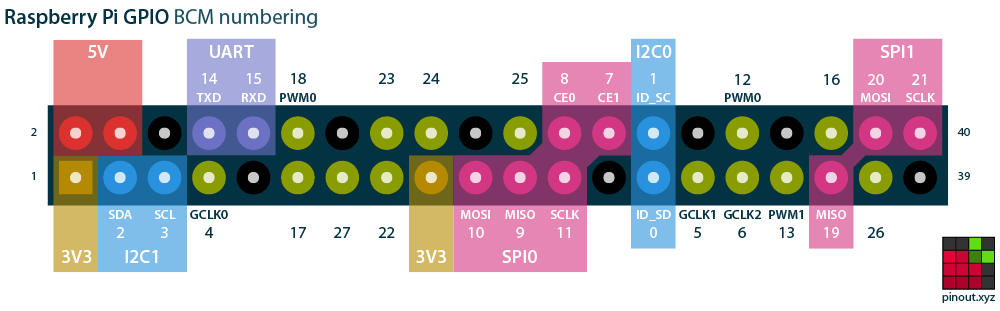
\includegraphics[scale = 0.35]{Figures/raspberry-pi-pinout.png}
    \caption{Esquema de pines Raspberry Pi}
    \label{fig:pinout_scheme}
\end{figure}

En primer lugar, se procede a la preparación de la pantalla. Se le quitan los separadores que unen la pcb a la pantalla per se y se atornilla la pantalla completa a la parte superior de la carcasa impresa previamente en 3D.

El siguiente paso es, instalar y cablear la placa controladora de la batería, en el espacio destinado para ello, realizar su cableado e instalar la batería sobre esta.

Se realiza en el siguiente paso la instalación del led que se hará directamente sobre la RPI.

A continuación se cablea el sensor de luz. Para ello será necesario conectar un conversor de señal analógico digital a los pines SDA y SCL, que nos permitirá comunicación mediante I2C\cite{i2c} con el sensor y posteriormente este al conversor.La mejor forma de anclarlo a la carcasa será utilizando un trozo de cinta de doble cara.

En ll siguiente paso, en la esquina libre restante de la carcasa, se instalará la batería Pi Sugar+ con el interruptor de encendido del dispositivo.

Se deberán conectar todos los cables en su debido lugar. 
Se han utilizado el conector LSI flexible y los pines 25 (masa) de la RPI y el pin de salida de voltaje a 5v de la batería para la pantalla. 
Para la alimentación se han utilizado los pines: 2 de la RPI (5v) conectado a la salida de 5v de la batería, 6 de la RPI (masa) con la masa de la batería, el pin 11 de la RPI con el SDAT de la batería y el 13 de la RPI con el SCLK de la batería. 
Con el led se han utilizado los pines 14 y 16 (masa) de la RPI. 
Para poder obtener información analógica del sensor de luminosidad se utilizará el conversor analógico digital que irá conectado a los pines 4(5V), 3 (SDA), 5 (SCL), 9 (masa), 20 (masa) con los pines VDD, SDA, SCL, masa y ADDR del conversor respectivamente.
Por último los pines para el sensor de luminosidad son: 4 de la RPI con VDD del sensor. A0 del conversor analógico digital con OUT del sensor, que debe estar puenteado con el 1M. -V y COM del sensor deben ir conectados al pin 7 de la RPI.
Se puede cerrar la carcasa con los cuatro tornillos restantes. Se facilita ahora el esquema de cableado final. Ver figura:\ref{fig:wiring_pi}.

\begin{figure}[H]
    \centering
    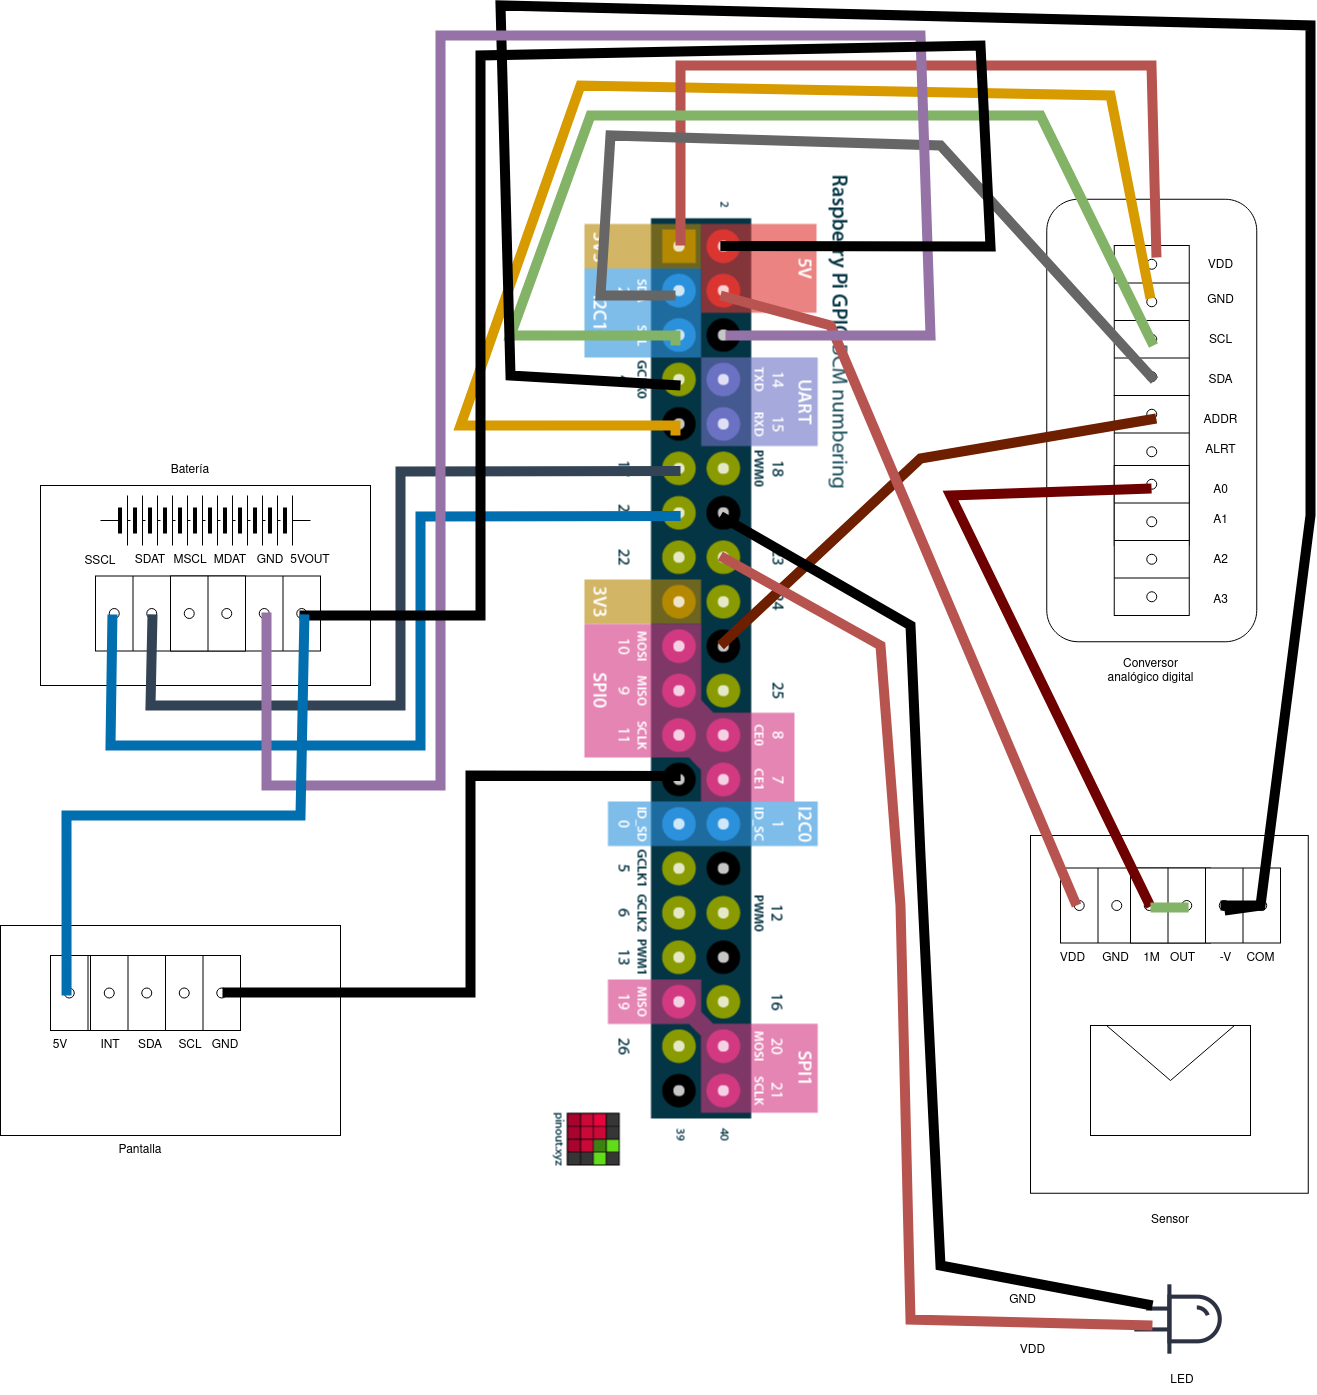
\includegraphics[scale = 0.25]{Figures/Wiring_Pi_sensor.png}
    \caption{Cableado completo.}
    \label{fig:wiring_pi}
\end{figure}

Para finalizar la instalación se instalara la tarjeta micro sd con el software previamente cargado en su ranura correspondiente.

* Para el prototipo se ha fabricado una nueva versión de la carcasa utilizando como molde la original a mano modificada anteriormente, y complementada con los componentes que a posteriori se instalarán en ella para la correcta medición de los espacios necesarios para los puertos de carga y la instalación del controlador de las baterías.

\section{Implementación}

En esta sección se describe el proceso de implementación del software del medidor de latencias, detallando las decisiones técnicas tomadas, los problemas encontrados y las soluciones aplicadas durante el desarrollo de cada módulo.

\subsection{Entorno de desarrollo y configuración inicial}

El desarrollo se ha realizado sobre Windows 11 con Qt Creator 16 como entorno de desarrollo integrado, utilizando Qt 6.11.1 con el compilador MinGW 13.1.0 (64 bits) para la compilación Desktop. Paralelamente, se ha verificado la compilación en Linux (Ubuntu) con Clang y GCC para garantizar la portabilidad del código.

La elección de \textbf{qmake} como sistema de construcción se debe a su integración nativa con Qt Creator y su capacidad para gestionar automáticamente el preprocesador de meta-objetos (MOC), la compilación de formularios (.ui), la generación de traducciones (.qm) y la detección condicional de plataforma (ARM vs x86-64).

Se configuró un proyecto SUBDIRS con dos sub-proyectos: la aplicación principal (\texttt{LatencyTester.pro}) y la batería de pruebas (\texttt{Tests.pro}), permitiendo al desarrollador elegir qué compilar en cada momento.

\subsubsection{Compilación cruzada para Raspberry Pi}

Se configuró un kit de compilación cruzada ARM GNU Toolchain que permite generar binarios para la Raspberry Pi directamente desde la máquina de desarrollo x86-64. El fichero \texttt{.pro} detecta automáticamente la arquitectura de destino y condiciona las dependencias:
\begin{itemize}
    \item En ARM: define \texttt{RASPBERRY\_PI}, enlaza \texttt{pigpio} y \texttt{libgpiod}, incluye el driver real del ADS1115.
    \item En Desktop: utiliza stubs que simulan las operaciones GPIO y ADC sin hardware real.
\end{itemize}

\subsubsection{Workaround para QCustomPlot con Qt 6.8+}

La biblioteca QCustomPlot 2.1.0 utiliza \texttt{Q\_GADGET} dentro de un namespace, lo cual es incompatible con la generación constexpr de metaobjetos introducida en Qt 6.8. Se resolvió definiendo \texttt{QT\_NO\_CONSTEXPR\_METAOBJECT\_DATA} en el \texttt{.pro} y parcheando manualmente el fichero \texttt{qcustomplot.h} para evitar el truco de la clase falsa que QCustomPlot usa para registrar enums en el sistema de meta-tipos. Además, se actualizaron las APIs deprecadas: \texttt{mirrored()} por \texttt{flipped()}, \texttt{toTimeSpec()} por \texttt{toTimeZone()}, y \texttt{startOfDay(Qt::TimeSpec)} por \texttt{startOfDay(QTimeZone)}.

\subsection{Arquitectura Core/GUI}

Se adoptó una arquitectura de separación estricta entre lógica de negocio (Core) y presentación (GUI). La motivación principal fue:
\begin{itemize}
    \item Facilitar las pruebas unitarias de la lógica sin necesidad de instanciar interfaz gráfica.
    \item Permitir la reutilización del Core en futuras versiones del producto (por ejemplo, una interfaz web).
    \item Reducir el acoplamiento entre módulos, mejorando la mantenibilidad.
\end{itemize}

Inicialmente, toda la funcionalidad residía en una única clase monolítica (\texttt{StartScreen}) que gestionaba las 8 pantallas, la navegación, la configuración, las traducciones y el control del sensor. Este diseño, heredado de la primera versión del prototipo, fue refactorizado completamente en la siguiente fase.

\subsection{Refactorización: de StartScreen monolítico a pantallas independientes}

El mayor esfuerzo de ingeniería del proyecto consistió en descomponer los más de 600 líneas de \texttt{startscreen.cpp} en clases independientes. El proceso se realizó de forma incremental:

\begin{enumerate}
    \item \textbf{HomeScreen}: extracción de los 4 botones de navegación del menú principal.
    \item \textbf{SettingsScreen}: extracción de los widgets de configuración (idioma, fuente, modos) con su lógica de Apply/Cancel.
    \item \textbf{HelpScreen} + \textbf{HelpInfoScreen}: separación del menú de ayuda y el visor de contenido.
    \item \textbf{RegistryScreen}: extracción del historial de mediciones (TreeView + acciones).
    \item \textbf{RegistryDisplayScreen}: visualización de mediciones guardadas con gráfica.
    \item \textbf{MeasureScreen}: extracción de la pantalla de mediciones con toda su lógica asíncrona.
    \item Eliminación completa de \texttt{StartScreen} y del enum \texttt{MenuScreen}.
\end{enumerate}

La clase \textbf{MainWindow} se creó como controlador central de navegación, utilizando un \texttt{QStackedWidget} con 7 pantallas indexadas. La comunicación entre pantallas se realiza exclusivamente mediante signals/slots de Qt, eliminando cualquier dependencia directa entre widgets.

\subsubsection{Dificultades encontradas}

\begin{itemize}
    \item \textbf{Dependencia circular RenamePopUp/StartScreen}: el popup de renombrar conectaba sus señales directamente al \texttt{StartScreen} en el constructor mediante un cast al padre. Se resolvió moviendo las conexiones al \texttt{RegistryScreen} que instancia el popup, desacoplando completamente ambas clases.
    \item \textbf{Traducción inglés→español al arranque}: al iniciar la aplicación en inglés y cambiar a español, la traducción no se aplicaba. El problema era que \texttt{removeTranslator} no disparaba \texttt{LanguageChange} si no había un translator instalado previamente. La solución fue crear un fichero de traducción identidad para español (donde source = translation) e instalarlo siempre, garantizando que el evento se emite en todos los casos.
    \item \textbf{Bloqueo de señales durante carga de ajustes}: al restaurar los valores de los widgets desde \texttt{AppSettings}, cada \texttt{setValue}/\texttt{setChecked} disparaba las señales de cambio, habilitando prematuramente el \texttt{QDialogButtonBox}. Se resolvió bloqueando las señales de los widgets durante la carga y restaurándolas después.
\end{itemize}

\subsection{Módulo AppSettings (Singleton de configuración)}

Se implementó como un singleton (\texttt{static AppSettings\& instance()}) que centraliza:
\begin{itemize}
    \item Carga y guardado de configuración mediante \texttt{QSettings} (registro en Windows, fichero ini en Linux).
    \item Almacenamiento de hojas de estilo (light/dark) y colores de modo daltónico.
    \item Emisión de señales granulares: solo se emite la señal del parámetro que realmente cambió al llamar a \texttt{applySettings()}.
\end{itemize}

El \texttt{MainWindow} escucha la señal \texttt{settingsApplied()} para re-aplicar temas, fuentes y modo daltónico de forma global a todos los hijos, excluyendo expresamente el botón de retroceso (que mantiene siempre 24pt bold amarillo).

\subsection{Módulo JsonOperator (Persistencia de mediciones)}

Gestiona la serialización de mediciones a formato JSON y su almacenamiento en disco. El formato elegido es sencillo y legible:
\begin{verbatim}
{ "Name": "...", "Date": "ISO8601",
  "TimeFactor": N, "Duration": N, "Latencies": [...] }
\end{verbatim}

\subsubsection{Bugs detectados y corregidos}

\begin{enumerate}
    \item \textbf{Lógica if invertida}: la función \texttt{saveMeasureToDisk()} tenía un \texttt{if(!mFile->open(...))} que provocaba que la escritura se intentase dentro del bloque de error. El fichero nunca se creaba realmente. Detectado por los tests unitarios.
    \item \textbf{Caracteres ilegales en nombres de fichero}: \texttt{QDateTime::toString(Qt::ISODate)} produce colons (e.g., \texttt{T08:00:00}) que Windows rechaza en nombres de fichero. Corregido reemplazando \texttt{:} por \texttt{-} antes de construir la ruta.
    \item \textbf{Memory leak}: cada llamada a \texttt{loadFileFromDisk()} o \texttt{saveMeasureToDisk()} creaba un nuevo \texttt{QFile} con \texttt{new} sin liberar el anterior. Detectado por AddressSanitizer en Linux. Corregido añadiendo \texttt{delete mFile;} antes de cada nueva asignación.
\end{enumerate}

\subsection{Módulo SensorOperator (Control del hardware)}

Controla el LED estimulador (GPIO 24) y el fotosensor (ADS1115 ADC vía I2C). La lógica implementada incluye:

\begin{description}
    \item[Calibración] 4 ciclos de parpadeo LED (500ms on/off). Durante la fase off se muestrean lecturas del fotosensor para establecer un baseline ambiental. El umbral de detección se fija en baseline + 20\%.
    \item[Medición] Para cada pulso: LED off (50ms estabilización), LED on, polling del sensor hasta superar el umbral (timeout 5s). La diferencia temporal es la latencia. Se registra -1 para mediciones fallidas.
    \item[Interrupción] Un flag atómico (\texttt{mStopMeasure}) permite interrumpir cualquier operación en curso desde el hilo de la GUI.
\end{description}

Las operaciones de calibración y medición se ejecutan en hilos background mediante \texttt{QtConcurrent::run()}, evitando bloquear la interfaz gráfica. Un \texttt{QFutureWatcher} notifica la finalización y dispara la actualización de la UI.

\subsubsection{Stubs para desarrollo Desktop}

Se crearon ficheros stub (\texttt{pigpio\_stub.h}, \texttt{ads1115rpi\_stub.h}) que implementan las mismas interfaces que las bibliotecas de hardware reales, pero con operaciones no-op. Esto permite compilar y probar toda la aplicación en un ordenador sin Raspberry Pi ni sensores conectados.

\subsection{Interfaz gráfica: pantalla de mediciones (MeasureScreen)}

La pantalla de mediciones es la más compleja de la aplicación. Incluye:

\begin{itemize}
    \item \textbf{Gráfica en tiempo real}: implementada con QCustomPlot. La función \texttt{plotMeasure()} utiliza paralelización mediante \texttt{QtConcurrent::run()} para datasets superiores a 100 puntos, dividiendo el filtrado de datos entre todos los núcleos disponibles.
    \item \textbf{Flash visual no-bloqueante}: un \texttt{QTimer} cicla colores en el botón activo (verde/oscuro durante operación, verde/rojo al finalizar). No utiliza busy-wait, preservando la responsividad de la interfaz.
    \item \textbf{Deshabilitación selectiva de widgets}: durante calibración o medición, todos los botones y sliders se deshabilitan excepto el botón Detener, que permite interrumpir la operación.
    \item \textbf{Sliders con valor numérico}: las etiquetas muestran en tiempo real el valor configurado con su unidad (\texttt{tr("Intervalo entre mediciones: \%1 ms")}), y se actualizan también al cambiar de idioma.
\end{itemize}

\subsection{Modos de visualización}

Se implementaron dos modos ortogonales de visualización:

\begin{description}
    \item[Modo nocturno (Dark Mode)] Hoja de estilo completa con fondo oscuro (\texttt{rgb(35,35,50)}), botones con bordes semitransparentes, combos, checkboxes y sliders con estilos coherentes. Se aplica a nivel de \texttt{MainWindow} (herencia CSS).
    \item[Modo daltónico] Paleta de alto contraste (fondo verde \texttt{rgb(82,183,136)}, botón atrás rojo \texttt{rgb(157,2,8)}). Tiene prioridad sobre el modo nocturno: se aplica después, sobreescribiendo los colores afectados.
\end{description}

Ambos modos persisten entre sesiones vía \texttt{QSettings}.

\subsection{Sistema de internacionalización (i18n)}

La aplicación soporta tres idiomas (español, inglés, polaco) mediante el sistema estándar de traducciones de Qt:

\begin{enumerate}
    \item Todas las cadenas visibles se marcan con \texttt{tr()}.
    \item Ficheros \texttt{.ts} (XML) contienen las traducciones organizadas por contexto (nombre de clase).
    \item La directiva \texttt{embed\_translations} de Qt 6 compila e incrusta los ficheros \texttt{.qm} directamente en el binario sin necesidad de ficheros \texttt{.qrc} adicionales.
    \item Cada pantalla implementa \texttt{changeEvent(QEvent::LanguageChange)} para llamar a \texttt{retranslateUi(this)} y actualizar textos dinámicos.
\end{enumerate}

\subsection{Manual de usuario integrado (HTML embebido)}

Se desarrolló una versión condensada del manual de usuario en formato HTML (uno por idioma) que se embebe en el binario mediante un fichero \texttt{.qrc}. La pantalla \texttt{HelpInfoScreen} utiliza un \texttt{QTextBrowser} para renderizar el HTML con navegación por anclas internas. El botón ``Manual de usuario'' en \texttt{HelpScreen} se habilita o deshabilita automáticamente según exista el recurso HTML para el idioma activo, verificado mediante \texttt{QFile::exists()} sobre la ruta \texttt{qrc:/}.

\subsection{Scripts de automatización}

Se desarrollaron scripts para Windows (PowerShell) y Linux (Bash) que automatizan:
\begin{itemize}
    \item Compilación en modo Release con paralelización (\texttt{-j8} / \texttt{-j\$(nproc)}).
    \item Generación de documentación Doxygen con diagramas SVG (Graphviz).
    \item Limpieza de artefactos de compilación.
\end{itemize}

Los scripts detectan automáticamente la presencia de las herramientas necesarias (\texttt{qmake}, \texttt{make}/\texttt{mingw32-make}, \texttt{doxygen}) e informan al usuario si alguna no está disponible.

\subsection{Detección de errores de memoria (AddressSanitizer)}

Se integró AddressSanitizer (ASan) en las compilaciones Debug sobre Linux. Los flags \texttt{-fsanitize=address -fno-omit-frame-pointer} se activan condicionalmente en el \texttt{.pro} mediante la directiva \texttt{linux \{\}}. En Windows con MinGW no se activa al no disponer de la librería \texttt{libasan}.

El análisis con ASan reveló una fuga de memoria real en \texttt{JsonOperator}: cada llamada a \texttt{loadFileFromDisk()} asignaba un nuevo \texttt{QFile} sin liberar el anterior, acumulando 448 bytes por operación. El resto de alertas correspondieron a falsos positivos de fontconfig (cache de fuentes del sistema) y pools internos de Qt.

\subsection{Pruebas unitarias}

Se implementó una batería completa de 147 tests unitarios distribuidos en 10 suites, cubriendo tanto la capa Core como la capa GUI:

\begin{itemize}
    \item \textbf{Core}: verificación de valores por defecto de estructuras de datos, persistencia de configuración con señales, serialización/deserialización JSON (incluyendo ficheros corruptos y campos faltantes), y validación de parámetros del sensor.
    \item \textbf{GUI}: instanciación de widgets, existencia y estado de botones/sliders, emisión de señales al interactuar con la interfaz (\texttt{QTest::mouseClick} + \texttt{QSignalSpy}), y verificación de la lógica Apply/Cancel en ajustes.
\end{itemize}

Las pruebas no requieren hardware ni display físico (se ejecutan offscreen) y detectaron tres bugs reales en producción que se corrigieron antes de la entrega.

\subsection{Configuración de la toolchain de compilación cruzada}

La configuración de la cadena de herramientas para compilación cruzada ARM64 resultó ser el mayor contratiempo técnico del proyecto. Se documentan a continuación las distintas aproximaciones intentadas y las dificultades encontradas en cada una.

\subsubsection{Aproximación 1: qmake con cross-compiler y sysroot de Docker}

El primer intento consistió en utilizar el \texttt{qmake} del Qt Online Installer (x86-64) pasando los compiladores cruzados como variables:

\begin{verbatim}
qmake LatencyTester.pro \
  "QMAKE_CC=aarch64-linux-gnu-gcc" \
  "QMAKE_CXX=aarch64-linux-gnu-g++" \
  "QMAKE_LINK=aarch64-linux-gnu-g++" \
  "QMAKE_CFLAGS+=--sysroot=$SYSROOT" \
  "QMAKE_LFLAGS+=--sysroot=$SYSROOT"
\end{verbatim}

\textbf{Problema}: qmake genera las rutas de las librerías Qt apuntando siempre a la instalación x86-64 del host (\texttt{gcc\_64/lib/}). El enlazador ARM64 rechaza estas librerías con el error \texttt{file in wrong format}. Se parcheó el Makefile con \texttt{sed} para reemplazar las rutas, pero al enlazar contra las librerías Qt 6.7 del sysroot (extraídas de los repositorios Debian ARM64) con las cabeceras de Qt 6.11 (del Online Installer), se produjeron cientos de \texttt{undefined reference} a funciones inexistentes en Qt 6.7.

\textbf{Conclusión}: la compilación cruzada con qmake requiere que la versión de Qt de las cabeceras y la de las librerías de enlace sean idénticas. No es viable mezclar versiones.

\subsubsection{Aproximación 2: compilación nativa dentro del contenedor Docker}

Se intentó compilar directamente dentro del contenedor Docker ARM64 (emulado con QEMU user-mode), que sí dispone de Qt 6.7 ARM64 coherente (headers + libs misma versión).

\textbf{Problema}: qmake ejecuta internamente \texttt{g++ -E -dM} para extraer las macros del compilador. Bajo emulación QEMU user-mode, la salida estándar del subproceso se altera, impidiendo que qmake parsee correctamente las macros. El error resultante es:
\begin{verbatim}
Variable QMAKE_CXX.COMPILER_MACROS is not defined.
Project ERROR: failed to parse default search paths
\end{verbatim}

\textbf{Conclusión}: qmake no funciona bajo emulación QEMU user-mode. Descartado.

\subsubsection{Aproximación 3 (adoptada): compilar Qt 6.11 desde fuente para ARM64}

La solución definitiva consiste en compilar la misma versión de Qt que se usa en el host (6.11.1) pero targeting ARM64. Esto garantiza coherencia total entre cabeceras y librerías. El proceso se automatizó mediante el script \texttt{build-qt6-arm64.sh} que:

\begin{enumerate}
    \item Descarga el código fuente completo de Qt 6.11.1 ($\sim$900 MB comprimido).
    \item Genera un fichero \texttt{CMake toolchain} que apunta al cross-compiler y al sysroot ARM64.
    \item Configura la build con CMake + Ninja, reutilizando las host tools del Online Installer.
    \item Compila todas las librerías Qt para ARM64 ($\sim$1--2 horas en un procesador de 4 núcleos).
    \item Instala en \texttt{/opt/Qt/6.11.1/arm64/} proporcionando un \texttt{qt-cmake} y \texttt{qmake} nativos para cross-compilación.
\end{enumerate}

Una vez instalada, la compilación del proyecto se reduce a:
\begin{verbatim}
/opt/Qt/6.11.1/arm64/bin/qmake LatencyTester.pro
make -j$(nproc)
\end{verbatim}

\subsubsection{Lecciones aprendidas}

\begin{itemize}
    \item La compilación cruzada de aplicaciones Qt requiere una versión de Qt compilada específicamente para la arquitectura destino. No es posible reutilizar las librerías de los repositorios de la distribución si la versión no coincide exactamente con las cabeceras del host.
    \item Las herramientas como \texttt{moc}, \texttt{uic}, \texttt{rcc} y \texttt{lrelease} deben ser las nativas del host (x86-64), mientras que las librerías de enlace deben ser ARM64.
    \item QEMU user-mode es útil para ejecutar binarios ARM64, pero no para compilar con qmake (problemas con la captura de stdout de subprocesos).
    \item El proceso de compilar Qt desde fuente, aunque largo, es determinista y solo debe realizarse una vez por versión de Qt utilizada.
\end{itemize}

\section{Pruebas y validación}

En esta sección se describe la infraestructura de pruebas establecida para validar el correcto funcionamiento del software del medidor de latencias. Se detallan las herramientas utilizadas, las distintas aproximaciones exploradas para emular el hardware destino, las dificultades encontradas y la configuración final adoptada.

\subsection{Estrategia de pruebas}

Se adoptó una estrategia de validación en tres niveles complementarios:

\begin{enumerate}
    \item \textbf{Pruebas unitarias} (automatizadas, sin hardware): verificación funcional de cada módulo de forma aislada, ejecutables en cualquier máquina de desarrollo.
    \item \textbf{Análisis de memoria} (automatizado, sin hardware): detección de fugas de memoria y accesos inválidos mediante instrumentación del binario.
    \item \textbf{Validación sobre plataforma destino} (o emulación de la misma): ejecución del binario ARM64 completo en un entorno equivalente a la Raspberry Pi para verificar el correcto funcionamiento gráfico y la integración de componentes.
\end{enumerate}

\subsection{Pruebas unitarias con QTest}

Se eligió QTest (Qt Test) como framework de pruebas unitarias por las siguientes razones:
\begin{itemize}
    \item Todo el código del proyecto depende de tipos Qt (\texttt{QString}, \texttt{QVector}, \texttt{QSettings}, signals/slots), lo que hace innecesaria la introducción de un framework externo como Google Test.
    \item QTest se integra nativamente con el event loop de Qt, permitiendo probar comportamientos asíncronos y señales.
    \item \texttt{QSignalSpy} permite verificar la emisión de señales de forma determinista.
    \item \texttt{QTest::mouseClick} y \texttt{QTest::keyClick} permiten simular interacción de usuario sobre widgets sin necesidad de display físico (ejecución offscreen).
\end{itemize}

\subsubsection{Arquitectura del sub-proyecto de tests}

Los tests se compilan como un binario independiente (\texttt{LatencyTesterTests}) mediante un sub-proyecto qmake (\texttt{Tests.pro}) que comparte las fuentes del proyecto principal pero añade las suites de test. La compilación de los tests se condiciona a la configuración Debug mediante un proyecto SUBDIRS en la raíz:

\begin{verbatim}
SUBDIRS += LatencyTester
CONFIG(debug, debug|release) {
    SUBDIRS += Tests
    Tests.depends = LatencyTester
}
\end{verbatim}

\subsubsection{Cobertura de pruebas}

Se implementaron 147 tests distribuidos en 10 suites, cubriendo ambas capas de la arquitectura:

\begin{table}[H]
\centering
\caption{Resumen de suites de pruebas unitarias}
\label{tab:test_suites}
\begin{tabular}{|p{4.5cm}|p{1cm}|p{7cm}|}
\hline
\textbf{Suite} & \textbf{Tests} & \textbf{Cobertura} \\ \hline
tst\_datamodel & 17 & Valores por defecto de structs, edge cases (duration=0, timeFactor negativo). \\ \hline
tst\_appsettings & 23 & Singleton, load/save QSettings, emisión de señales, stylesheets light/dark/daltonic. \\ \hline
tst\_jsonoperator & 14 & Parse JSON valido/invalido, save/load round-trip, ficheros corruptos, campos faltantes. \\ \hline
tst\_sensoroperator & 14 & Validación parametros, interrupción con stop, calibración con stubs, timeout. \\ \hline
tst\_homescreen & 10 & Botones de navegación, emisión de señales, existencia de widgets. \\ \hline
tst\_measurescreen & 14 & Botones, sliders (rango, labels), gráfica, estado stopButton deshabilitado. \\ \hline
tst\_settingsscreen & 20 & Apply/cancel, sincronización widgets-settings, habilitación buttonBox. \\ \hline
tst\_helpscreen & 11 & Botón manual habilitado/deshabilitado según recurso HTML del idioma. \\ \hline
tst\_registryscreen & 10 & TreeView con modelo, botones de acción, señales. \\ \hline
tst\_registrydisplayscreen & 14 & displayMeasure con datos mock, ploteo, edge case latencies vacías. \\ \hline
\end{tabular}
\end{table}

\subsubsection{Ejecución de los tests}

\begin{verbatim}
# Todos los tests
./LatencyTesterTests

# Un test especifico por nombre de funcion
./LatencyTesterTests test_saveMeasure_roundTrip

# Verbose (muestra cada test)
./LatencyTesterTests -v1

# Exportar resultados en XML
./LatencyTesterTests -o results.xml,xml
\end{verbatim}

\subsection{Análisis de memoria con AddressSanitizer}

Para la detección de fugas de memoria, desbordamientos de buffer y accesos a memoria liberada, se integró AddressSanitizer (ASan) en las compilaciones Debug sobre Linux. Los flags de compilación se activan condicionalmente en el fichero \texttt{.pro}:

\begin{verbatim}
linux {
    QMAKE_CXXFLAGS += -fsanitize=address -fno-omit-frame-pointer
    QMAKE_LFLAGS += -fsanitize=address
}
\end{verbatim}

En Windows con MinGW no se activa al no disponer de la librería \texttt{libasan} en la distribución de MinGW que empaqueta Qt.

\subsubsection{Limitación en Windows}

La versión de MinGW 13.1.0 incluida con Qt 6.11 no distribuye \texttt{libasan}. El intento de compilar con \texttt{-fsanitize=address} en Windows produce el error:
\begin{verbatim}
ld.exe: cannot find -lasan: No such file or directory
\end{verbatim}

Se resolvió condicionando los flags a la plataforma Linux, donde GCC/Clang sí incluyen ASan de serie.

\subsection{Entorno de emulación: aproximaciones exploradas}

Para validar el binario ARM64 sin disponer permanentemente de la Raspberry Pi física, se exploraron tres aproximaciones de emulación, cada una con distinto nivel de fidelidad y complejidad.

\subsubsection{Aproximación 1: QEMU con máquina raspi3b}

Se intentó emular directamente la Raspberry Pi 3 Model B con QEMU utilizando la máquina \texttt{raspi3b}:

\begin{verbatim}
qemu-system-aarch64 -machine raspi3b -cpu cortex-a53 -m 1024 \
  -kernel kernel8.img -dtb bcm2710-rpi-3-b.dtb \
  -drive file=imagen.img,format=raw,if=sd ...
\end{verbatim}

\textbf{Dificultades encontradas}:
\begin{itemize}
    \item La extracción del kernel de la imagen requiere montar la partición boot con offset calculado manualmente (\texttt{mount -o loop,offset=\$((Start*512))}). Los comandos \texttt{losetup --partscan} no funcionaban correctamente en todas las distribuciones.
    \item Las imágenes recientes de Raspi OS utilizan sectores de 4096 bytes en lugar de 512, generando warnings de \texttt{fdisk} y offsets incorrectos si no se tiene en cuenta.
    \item El formato qcow2 no es compatible con la interfaz SD emulada de la máquina \texttt{raspi3b}: se requiere formato raw con tamaño potencia de 2.
    \item La máquina \texttt{raspi3b} de QEMU es altamente inestable con kernels recientes: el proceso QEMU finalizaba inmediatamente sin mostrar salida ni error, al no ser compatible el \texttt{kernel8.img} de imágenes Raspi OS modernas con la emulación limitada del hardware (GPU VideoCore no emulada).
    \item No emula GPU, por lo que las aplicaciones gráficas no pueden renderizarse de forma nativa.
\end{itemize}

Se descartó esta aproximación por su inestabilidad y la imposibilidad de ejecutar la interfaz gráfica.

\subsubsection{Aproximación 2: QEMU con máquina virt}

Se exploró la máquina genérica \texttt{virt} de QEMU, más estable que \texttt{raspi3b}:

\begin{verbatim}
qemu-system-aarch64 -machine virt -cpu cortex-a72 -m 2048 \
  -drive file=imagen.img,format=raw ...
\end{verbatim}

Aunque más estable, presentaba las mismas limitaciones gráficas: para ver la GUI se requiere configurar un dispositivo VNC (\texttt{-device virtio-gpu-pci -display vnc=:0}), convirtiendo la configuración en algo equivalente a la solución Docker pero con mayor complejidad de setup.

\subsubsection{Aproximación 3: Docker con emulación multiarch (solución adoptada)}

Finalmente se adoptó Docker con emulación ARM64 vía \texttt{qemu-user-static} como entorno de pruebas, por su simplicidad, reproducibilidad y capacidad de soportar GUI vía VNC:

\begin{itemize}
    \item \textbf{Emulación transparente}: Docker utiliza \texttt{binfmt\_misc} del kernel Linux para ejecutar binarios ARM64 de forma transparente mediante QEMU user-mode, sin necesidad de emular una máquina completa.
    \item \textbf{Reproducible}: un \texttt{Dockerfile} define exactamente el entorno de ejecución (Debian Bookworm ARM64 con las librerías Qt 6 de runtime).
    \item \textbf{GUI via VNC}: el contenedor ejecuta Xvfb (framebuffer virtual a 800x480) + x11vnc, permitiendo visualizar la aplicación desde cualquier cliente VNC conectado a \texttt{localhost:5900}.
    \item \textbf{Valgrind integrado}: disponible directamente dentro del contenedor para análisis de memoria sobre el binario ARM64.
\end{itemize}

\subsubsection{Scripts de automatización del entorno Docker}

Se creó el script \texttt{docker-rpi.sh} que automatiza toda la gestión del contenedor:

\begin{verbatim}
./docker-rpi.sh setup      # Instala Docker + habilita ARM64
./docker-rpi.sh build      # Construye la imagen del contenedor
./docker-rpi.sh run        # Lanza con VNC en puerto 5900
./docker-rpi.sh shell      # Abre bash en el contenedor
./docker-rpi.sh valgrind   # Ejecuta Valgrind sobre el binario
./docker-rpi.sh stop       # Detiene el contenedor
./docker-rpi.sh clean      # Elimina contenedor e imagen
\end{verbatim}

El \texttt{Dockerfile} incluye:
\begin{itemize}
    \item Librerías Qt 6 runtime (Widgets, Concurrent, PrintSupport, GUI, OpenGL).
    \item Xvfb configurado a 800x480x24 (resolución de la pantalla táctil del dispositivo).
    \item x11vnc como servidor VNC sin contraseña (entorno de desarrollo local).
    \item Valgrind para análisis de memoria.
    \item Punto de entrada (\texttt{docker-entrypoint.sh}) que arranca automáticamente el framebuffer y el servidor VNC al iniciar el contenedor.
\end{itemize}

\subsubsection{Pasos para establecer el entorno}

\begin{enumerate}
    \item Instalar Docker en la máquina Linux de desarrollo:
    \begin{verbatim}
    curl -fsSL https://get.docker.com | sh
    sudo usermod -aG docker $USER
    \end{verbatim}
    \item Habilitar la emulación ARM64:
    \begin{verbatim}
    docker run --rm --privileged \
      multiarch/qemu-user-static --reset -p yes
    \end{verbatim}
    \item Construir la imagen:
    \begin{verbatim}
    cd LatencyTester/Scripts/Linux
    ./docker-rpi.sh build
    \end{verbatim}
    \item Lanzar el contenedor con VNC:
    \begin{verbatim}
    ./docker-rpi.sh run
    \end{verbatim}
    \item Conectar un cliente VNC a \texttt{localhost:5900} para visualizar la pantalla emulada de 800x480.
    \item Dentro del contenedor, ejecutar el binario ARM64 compilado con cross-toolchain:
    \begin{verbatim}
    cd /app
    ./LatencyTester
    \end{verbatim}
\end{enumerate}

\subsection{Resumen del entorno de validación}

\begin{table}[H]
\centering
\caption{Herramientas de validación utilizadas}
\label{tab:validation_tools}
\begin{tabular}{|p{3.5cm}|p{3cm}|p{6.5cm}|}
\hline
\textbf{Herramienta} & \textbf{Plataforma} & \textbf{Propósito} \\ \hline
QTest & Windows + Linux & Pruebas unitarias automatizadas (147 tests, Core + GUI) \\ \hline
AddressSanitizer & Linux & Detección de fugas de memoria y accesos inválidos \\ \hline
Docker + qemu-user & Linux & Emulación ARM64 para ejecución del binario destino \\ \hline
Xvfb + x11vnc & Docker ARM64 & Visualización gráfica de la aplicación vía VNC \\ \hline
Valgrind & Docker ARM64 & Análisis profundo de memoria sobre el binario ARM \\ \hline
\end{tabular}
\end{table}

\chapter{Resumen}

\chapter{Conclusiones y trabajo futuro}

\section{Conclusiones}

\section{Trabajo futuro}

\chapter{Agradecimientos}

Son muchas las personas que han contribuido tanto con aportaciones físicas, como con ideas a la realización de este proyecto de Medición de latencias para sistemas de videovigilancia críticos y es por ello que quiero dedicar estas líneas del documento para una mención y muestra de gratitud.

En primer lugar, a Arturo Hernandez Rico, mi jefe de proyectos en GTD Defense \& Security, por la idea de llevar a término este aparato y una serie de alternativas ofrecidas. A continuación agradezco al Dr. Andrés Yañez Escolano de la Escuela Superior de Ingeniería del Campus de Puerto Real, el prestamo de una placa Raspberry Pi 3 Model B junto con una tarjeta de memoria durante la crisis de los semiconductores acaecida en los últimos meses, la cual ha convertido en una auténtica odisea y a precios desorbitados conseguir una pieza de hardware como la mencionada anteriormente para poder comenzar con el proyecto. Agradecer también a mi tutor Dr. Gabriel Guerrero Contreras por todos los buenos consejos, recomendaciones y disponibilidad facilitadas durante este ejercicio. 
Aunque sin participación directa, me gustaría agradecer a mi familia y amigos por los ánimos proporcionados para acabar el proyecto. Al Dr. Alberto Paramio Leiva por realizarme una revisión con una opinión sincera del proyecto una vez terminado el documento y la implementación. En especial, a mi prometida, Ana Pastor Muñoz, que ha aguantado sin poder disfrutar completamente sus vacaciones para que pueda sentarme a desarrollarlo y estudiar, por la paciencia que ha tenido conmigo, el esfuerzo realizado y todo el apoyo que me ha brindado, gracias de corazón.

En último lugar, y aunque no les conozca en persona, quiero agradecer a Jim, miembro del foro de Raspberry Pi, toda su asistencia a la hora de ayudarme a conseguir una compilación cruzada para el proyecto alineada con mis deseos, y a todos esos programadores de bibliotecas de funciones anónimos en muchos casos de los que he podido tomar parte de su altruista trabajo para incorporar a este proyecto. A todos vosotros, sinceramente, gracias.

\appendix

\chapter{Manual de instalación}

Este apéndice describe los procedimientos necesarios para compilar, instalar y desplegar el software del medidor de latencias en las distintas plataformas soportadas. Se detallan tres escenarios: compilación para desarrollo local (Desktop), compilación y ejecución en el entorno Docker ARM64, y despliegue en la Raspberry Pi física.

% =========================================================================
\section{Requisitos previos}

\begin{table}[H]
\centering
\caption{Requisitos de software por plataforma}
\label{tab:install_requirements}
\begin{tabular}{|p{4cm}|p{4cm}|p{5cm}|}
\hline
\textbf{Componente} & \textbf{Windows} & \textbf{Linux} \\ \hline
Qt Framework & 6.11+ (MinGW 64-bit) & 6.11+ (GCC/Clang) \\ \hline
Compilador & MinGW 13+ (incluido con Qt) & GCC 11+ o Clang 15+ \\ \hline
Git & 2.40+ & 2.40+ \\ \hline
Docker & --- (no necesario) & 24+ (para emulación ARM64) \\ \hline
Doxygen & 1.9+ (opcional, docs) & 1.9+ (opcional, docs) \\ \hline
Graphviz & 8+ (opcional, diagramas) & 8+ (opcional, diagramas) \\ \hline
\end{tabular}
\end{table}

% =========================================================================
\section{Compilación Desktop (desarrollo local)}

La compilación Desktop utiliza stubs que simulan el hardware (GPIO, ADC), permitiendo desarrollar y probar la interfaz completa sin dispositivo físico.

\subsection{Windows}

\begin{enumerate}
    \item Instalar Qt 6.11 con el componente MinGW 64-bit mediante Qt Online Installer.
    \item Clonar el repositorio con submódulos:
    \begin{verbatim}
    git clone --recurse-submodules <url-repositorio>
    \end{verbatim}
    \item Abrir \texttt{latency\_tester.pro} (el de la raíz) en Qt Creator.
    \item Seleccionar el kit \texttt{Desktop Qt 6.11 MinGW 64-bit}.
    \item Build $\rightarrow$ Build All.
\end{enumerate}

Alternativamente, desde línea de comandos (PowerShell):
\begin{verbatim}
cd LatencyTester
qmake LatencyTester.pro "CONFIG+=release"
mingw32-make -j8
\end{verbatim}

\subsection{Linux}

\begin{enumerate}
    \item Instalar Qt 6.11 y las dependencias de desarrollo:
    \begin{verbatim}
    sudo apt install qt6-base-dev qt6-tools-dev-tools \
      qt6-virtualkeyboard-dev libqt6printsupport6 \
      libgl1-mesa-dev make g++
    \end{verbatim}
    \item Clonar y compilar:
    \begin{verbatim}
    git clone --recurse-submodules <url-repositorio>
    cd latency_tester/LatencyTester
    qmake LatencyTester.pro "CONFIG+=release"
    make -j$(nproc)
    \end{verbatim}
\end{enumerate}

El binario resultante se encuentra en el directorio de build (e.g., \texttt{release/LatencyTester} en Linux o \texttt{release\textbackslash LatencyTester.exe} en Windows).

% =========================================================================
\section{Entorno Docker ARM64 (emulación Raspberry Pi)}

Docker con emulación multiarch permite compilar y ejecutar el binario ARM64 en cualquier máquina Linux x86-64, sin necesidad de hardware Raspberry Pi.

\subsection{Principio de funcionamiento}

Docker utiliza \texttt{binfmt\_misc} del kernel Linux junto con QEMU en modo usuario (\texttt{qemu-user-static}) para interceptar la ejecución de binarios ARM64 y traducir las instrucciones a x86-64 de forma transparente. Esto permite que un contenedor Docker ARM64 se ejecute nativamente sobre un host x86-64.

\subsection{Instalación del entorno}

\begin{enumerate}
    \item \textbf{Instalar Docker} (si no está instalado):
    \begin{verbatim}
    curl -fsSL https://get.docker.com | sh
    sudo usermod -aG docker $USER
    # Cerrar sesión y volver a entrar
    \end{verbatim}
    
    \item \textbf{Habilitar emulación ARM64} (solo una vez por reinicio del host):
    \begin{verbatim}
    docker run --rm --privileged \
      multiarch/qemu-user-static --reset -p yes
    \end{verbatim}
    
    \item \textbf{Construir la imagen del contenedor}:
    \begin{verbatim}
    cd LatencyTester/Scripts/Linux
    ./docker-rpi.sh build
    \end{verbatim}
    
    Este comando construye una imagen basada en Debian Bookworm ARM64 que incluye:
    \begin{itemize}
        \item Librerías Qt 6 de runtime (Widgets, Concurrent, PrintSupport, GUI, OpenGL).
        \item Xvfb configurado a 800$\times$480 (resolución de la pantalla del dispositivo).
        \item x11vnc como servidor VNC para visualización remota.
        \item Valgrind para análisis de memoria.
    \end{itemize}
\end{enumerate}

\subsection{Compilación para ARM64 (cross-compilation en el host)}

Debido a una limitación conocida de qmake bajo emulación QEMU user-mode (qmake no puede parsear la salida de macros del compilador cuando \texttt{g++} se ejecuta a través de QEMU), la compilación debe realizarse en el host Linux nativo utilizando un compilador cruzado. El contenedor Docker se utiliza exclusivamente para la ejecución y las pruebas del binario resultante.

\begin{enumerate}
    \item Instalar el compilador cruzado ARM64 en el host:
    \begin{verbatim}
    sudo apt install gcc-aarch64-linux-gnu g++-aarch64-linux-gnu
    \end{verbatim}
    
    \item Compilar el proyecto indicando a qmake los compiladores cruzados:
    \begin{verbatim}
    cd latency_tester/LatencyTester
    qmake6 LatencyTester.pro \
      "QMAKE_CC=aarch64-linux-gnu-gcc" \
      "QMAKE_CXX=aarch64-linux-gnu-g++" \
      "QMAKE_LINK=aarch64-linux-gnu-g++"
    make -j$(nproc)
    \end{verbatim}
    
    El binario resultante (\texttt{LatencyTester}) es un ejecutable ELF nativo ARM64.
\end{enumerate}

\subsection{Ejecución en el contenedor Docker con interfaz gráfica (VNC)}

Una vez compilado el binario ARM64 en el host, se ejecuta dentro del contenedor Docker que proporciona las librerías Qt de runtime y el entorno gráfico emulado:

\begin{verbatim}
./docker-rpi.sh run

# Dentro del contenedor:
cd /app
./LatencyTester
\end{verbatim}

Conectar un cliente VNC (TigerVNC, Remmina, RealVNC) a \texttt{localhost:5900} para visualizar la pantalla emulada de 800$\times$480 píxeles.

\textbf{Nota sobre la limitación de qmake bajo QEMU}: el error \texttt{Variable QMAKE\_CXX.COMPILER\_MACROS is not defined} se produce porque qmake ejecuta internamente \texttt{g++ -E -dM} para extraer las macros del compilador. Cuando \texttt{g++} se ejecuta a través de QEMU user-mode, la emulación altera sutilmente la salida estándar del subproceso, impidiendo que qmake la parsee correctamente. La solución adoptada (compilar en el host con cross-compiler y ejecutar en el contenedor) evita este problema al no invocar qmake bajo emulación.

\subsection{Script de gestión docker-rpi.sh}

El script \texttt{docker-rpi.sh} automatiza todas las operaciones del contenedor:

\begin{table}[H]
\centering
\caption{Comandos del script docker-rpi.sh}
\label{tab:docker_commands}
\begin{tabular}{|l|p{9cm}|}
\hline
\textbf{Comando} & \textbf{Descripción} \\ \hline
\texttt{setup} & Instala Docker y habilita la emulación ARM64 mediante qemu-user-static. \\ \hline
\texttt{build} & Construye la imagen Docker ARM64 a partir del Dockerfile. \\ \hline
\texttt{run} & Lanza el contenedor con servidor VNC en el puerto 5900 y monta el proyecto en \texttt{/app}. \\ \hline
\texttt{shell} & Abre una sesión Bash interactiva dentro del contenedor (sin VNC). \\ \hline
\texttt{valgrind} & Ejecuta Valgrind con \texttt{--leak-check=full} sobre el binario en modo offscreen. \\ \hline
\texttt{stop} & Detiene el contenedor en ejecución. \\ \hline
\texttt{clean} & Elimina el contenedor y la imagen Docker del sistema. \\ \hline
\end{tabular}
\end{table}

% =========================================================================
\section{Despliegue en Raspberry Pi (producción)}

Para la instalación en el hardware de destino se requiere una compilación cruzada o una compilación nativa en la propia Raspberry Pi.

\subsection{Compilación cruzada desde Linux}

\begin{enumerate}
    \item Instalar el compilador cruzado ARM:
    \begin{verbatim}
    sudo apt install gcc-aarch64-linux-gnu g++-aarch64-linux-gnu
    \end{verbatim}
    
    \item Obtener el sysroot de la Raspberry Pi (bibliotecas y cabeceras del sistema):
    \begin{verbatim}
    rsync -avz pi@<ip-rpi>:/usr/lib /opt/rpi-sysroot/usr/
    rsync -avz pi@<ip-rpi>:/usr/include /opt/rpi-sysroot/usr/
    rsync -avz pi@<ip-rpi>:/lib /opt/rpi-sysroot/
    \end{verbatim}
    
    \item Configurar un kit de compilación en Qt Creator:
    \begin{itemize}
        \item Compilador C: \texttt{/usr/bin/aarch64-linux-gnu-gcc}
        \item Compilador C++: \texttt{/usr/bin/aarch64-linux-gnu-g++}
        \item Sysroot: \texttt{/opt/rpi-sysroot}
        \item Qt version: Qt 6 compilado para ARM (necesario compilar Qt desde fuente o usar distribución precompilada)
    \end{itemize}
    
    \item Compilar con el kit ARM seleccionado en Qt Creator, o desde la línea de comandos con el qmake ARM.
\end{enumerate}

\subsection{Transferencia a la Raspberry Pi}

\begin{verbatim}
scp LatencyTester pi@<ip-rpi>:/home/pi/LatencyTester/bin/
\end{verbatim}

\subsection{Configuración de arranque automático}

Para que la aplicación se ejecute al encender el dispositivo, se configura un servicio systemd:

\begin{verbatim}
# /etc/systemd/system/latencytester.service
[Unit]
Description=LatencyTester Application
After=multi-user.target

[Service]
Type=simple
User=pi
Environment=QT_QPA_PLATFORM=linuxfb
ExecStart=/home/pi/LatencyTester/bin/LatencyTester
Restart=on-failure

[Install]
WantedBy=multi-user.target
\end{verbatim}

Activar el servicio:
\begin{verbatim}
sudo systemctl enable latencytester
sudo systemctl start latencytester
\end{verbatim}

La variable \texttt{QT\_QPA\_PLATFORM=linuxfb} indica a Qt que renderice directamente sobre el framebuffer de la pantalla táctil, sin necesidad de X11 ni Wayland.

% =========================================================================
\section{Verificación de la instalación}

Tras la instalación, verificar:
\begin{enumerate}
    \item La aplicación arranca y muestra la pantalla de inicio.
    \item La pantalla táctil responde a la interacción.
    \item Los ajustes se persisten entre reinicios.
    \item El LED y el fotosensor responden a la calibración.
    \item Las mediciones se almacenan correctamente en la carpeta \texttt{Measures/}.
\end{enumerate}

\chapter{Manual de usuario}

Este capítulo constituye la guía de uso del medidor de latencias. Está dirigido al operador final del equipo y asume que el dispositivo ya se encuentra correctamente ensamblado y encendido. Para instrucciones de montaje e instalación, consulte el Apéndice A (Manual de instalación).

% =========================================================================
\section{Indicaciones de seguridad}

\begin{itemize}
    \item No exponga el equipo a líquidos, humedad excesiva ni temperaturas superiores a 40~°C.
    \item No dirija el LED estimulador directamente a los ojos. Aunque su potencia es baja, la exposición prolongada puede causar molestias visuales.
    \item Utilice únicamente la batería y el cargador especificados por el fabricante (PiSugar 3+ o equivalente, 5~V / 3~A).
    \item No abra la carcasa del equipo mientras esté conectado a la corriente eléctrica.
    \item Ante cualquier comportamiento anómalo (calentamiento excesivo, olor a quemado, pantalla en blanco prolongado), desconecte la alimentación inmediatamente.
\end{itemize}

% =========================================================================
\section{Descripción general del equipo}

El medidor de latencias es un instrumento portátil diseñado para cuantificar el retardo de vídeo en sistemas de videovigilancia. Su principio de funcionamiento es el siguiente:

\begin{enumerate}
    \item Un LED de alta luminancia emite un pulso de luz hacia la cámara del sistema bajo prueba.
    \item La cámara captura el pulso y lo transmite al monitor.
    \item Un fotosensor adosado al monitor detecta cuándo se reproduce el estímulo luminoso.
    \item El equipo calcula la diferencia temporal entre la emisión y la detección: esa diferencia es la \textbf{latencia del sistema}.
\end{enumerate}

\subsection{Componentes externos}

\begin{description}
    \item[Pantalla táctil (frontal)] Pantalla capacitiva de 7 pulgadas. Es el único medio de interacción con el equipo.
    \item[LED estimulador (lateral)] Diodo emisor de luz de alta luminancia. Se enciende automáticamente durante las mediciones.
    \item[Fotosensor (lateral opuesto)] Sensor óptico con ventana receptora. Debe orientarse hacia el monitor del sistema bajo prueba.
    \item[Puerto USB-C (inferior)] Carga de batería y alimentación externa.
    \item[Indicador de carga (inferior)] LED de estado de batería (verde = cargado, rojo = cargando).
\end{description}

% =========================================================================
\section{Encendido y apagado}

\subsection{Encendido}
Mantenga pulsado el botón de encendido durante 2 segundos. La pantalla mostrará brevemente el logotipo del sistema operativo y, a continuación, la pantalla de inicio de la aplicación.

\subsection{Apagado}
Mantenga pulsado el botón de retroceso (\textbf{←}) en la pantalla de inicio durante 3 segundos. El equipo guardará la configuración actual y se apagará de forma segura.

\textbf{Nota:} No desconecte la alimentación de forma abrupta. Podría dañar los datos de mediciones almacenados.

% =========================================================================
\section{Pantalla de inicio}

Al arrancar la aplicación se presenta el menú principal con cuatro botones:

\begin{description}
    \item[Comenzar medición] Accede a la pantalla de toma de mediciones (Sección~\ref{sec:manual_medicion}).
    \item[Historial de mediciones] Consulta las mediciones anteriores guardadas en el equipo (Sección~\ref{sec:manual_historial}).
    \item[Ajustes] Configura el idioma, tamaño de fuente y modos de visualización (Sección~\ref{sec:manual_ajustes}).
    \item[Ayuda] Muestra información general del equipo y acceso al presente manual (Sección~\ref{sec:manual_ayuda}).
\end{description}

Todas las pantallas secundarias disponen de un botón de retroceso amarillo (\textbf{←}) en la esquina superior izquierda que devuelve a la pantalla anterior.

% =========================================================================
\section{Toma de mediciones}
\label{sec:manual_medicion}

Esta es la pantalla principal de trabajo. Contiene los siguientes elementos:

\begin{description}
    \item[Gráfica de latencias] Área central donde se visualizan los resultados en tiempo real. El eje horizontal representa el tiempo transcurrido (en segundos) y el eje vertical la latencia medida (en milisegundos).
    \item[Botón ``Calibrar''] Inicia el proceso de calibración del fotosensor.
    \item[Botón ``Comenzar''] Inicia la toma de mediciones.
    \item[Botón ``Detener''] Interrumpe una medición o calibración en curso. Solo está activo durante una operación.
    \item[Deslizador ``Intervalo entre mediciones''] Configura el tiempo de espera entre pulsos consecutivos (100--2000~ms).
    \item[Deslizador ``Duración''] Configura la duración total del ensayo (10--600~s).
\end{description}

\subsection{Procedimiento de calibración}
\label{sec:manual_calibracion}

La calibración adapta el umbral del fotosensor a las condiciones de iluminación ambiental. \textbf{Debe realizarse siempre antes de la primera medición} y repetirse cada vez que cambien las condiciones de luz del entorno.

\begin{enumerate}
    \item Coloque el fotosensor orientado hacia la zona del monitor donde se proyectará el estímulo.
    \item Pulse \textbf{Calibrar}.
    \item El LED del equipo parpadeará de forma intermitente durante el proceso (4 ciclos de 1 segundo). No mueva el equipo durante esta fase.
    \item Si la calibración es satisfactoria, el botón \textbf{Calibrar} parpadeará en \textcolor{green}{verde} durante 3 segundos.
    \item Si falla, parpadeará en \textcolor{red}{rojo}. Revise la orientación del sensor y vuelva a intentarlo.
\end{enumerate}

\textbf{Nota:} Durante la calibración, la interfaz se deshabilita temporalmente. Puede pulsar \textbf{Detener} en cualquier momento para cancelar.

\subsection{Procedimiento de medición}

\begin{enumerate}
    \item Asegúrese de haber completado una calibración satisfactoria (ver Sección~\ref{sec:manual_calibracion}).
    \item Ajuste el \textbf{intervalo entre mediciones} según la precisión deseada:
    \begin{itemize}
        \item Valores bajos (100--300~ms): mayor resolución temporal, genera más datos.
        \item Valores altos (1000--2000~ms): menor resolución, útil para ensayos largos.
    \end{itemize}
    \item Ajuste la \textbf{duración} del ensayo según las necesidades.
    \item Dirija el LED hacia la cámara del sistema bajo prueba y el fotosensor hacia su monitor.
    \item Pulse \textbf{Comenzar}.
    \item El botón \textbf{Comenzar} parpadeará en verde mientras la medición esté en curso.
    \item Al finalizar:
    \begin{itemize}
        \item Si ha sido satisfactoria: el botón parpadea en verde y se muestra la gráfica de resultados.
        \item Si ha habido errores: el botón parpadea en rojo.
    \end{itemize}
    \item Los resultados se almacenan automáticamente en la memoria interna del equipo.
\end{enumerate}

\textbf{Nota:} Pulse \textbf{Detener} en cualquier momento para interrumpir la medición. Los datos recogidos hasta ese instante no se guardarán.

\subsection{Interpretación de la gráfica}

\begin{itemize}
    \item Cada punto representa una medición individual de latencia.
    \item La línea conecta los puntos con estilo escalón (step-right), facilitando la lectura de valores constantes.
    \item La latencia media se utiliza para ajustar automáticamente el rango vertical.
    \item En modo daltónico, los colores de la gráfica cambian a combinaciones de alto contraste (rojo/verde oscuro).
\end{itemize}

% =========================================================================
\section{Historial de mediciones}
\label{sec:manual_historial}

La pantalla de historial presenta una lista con todas las mediciones almacenadas en el equipo, organizadas por nombre de fichero.

\subsection{Acciones disponibles}

\begin{description}
    \item[Comprobar] Seleccione una medición de la lista y pulse \textbf{Comprobar} para visualizar su gráfica y datos asociados (nombre, fecha, latencia media, intervalo).
    \item[Borrar] Elimina permanentemente la medición seleccionada. Esta acción no se puede deshacer.
    \item[Renombrar] Abre una ventana emergente donde puede introducir un nuevo nombre para la medición seleccionada.
\end{description}

\subsection{Pantalla de visualización}

Al pulsar \textbf{Comprobar}, se muestra la pantalla de detalle con:

\begin{itemize}
    \item Gráfica de la medición almacenada (idéntica a la visualización en tiempo real).
    \item Cuatro campos informativos organizados en dos columnas:
    \begin{itemize}
        \item \textbf{Nombre}: identificador de la medición.
        \item \textbf{Fecha}: fecha y hora en que se realizó.
        \item \textbf{Latencia (ms)}: valor medio de latencia obtenido.
        \item \textbf{Intervalo (ms)}: intervalo entre pulsos utilizado.
    \end{itemize}
\end{itemize}

% =========================================================================
\section{Ajustes}
\label{sec:manual_ajustes}

La pantalla de ajustes permite personalizar la experiencia de uso del equipo.

\begin{description}
    \item[Idioma] Selector desplegable con tres opciones: Español, English, Polski. El cambio es inmediato tras pulsar \textbf{Aplicar}.
    \item[Tamaño de fuente] Deslizador con rango de 9 a 15 puntos. La etiqueta muestra el valor actual en tiempo real.
    \item[Modo daltónicos] Casilla de verificación que activa una paleta de colores de alto contraste optimizada para usuarios con deficiencias en la percepción cromática.
    \item[Modo nocturno] Casilla de verificación que activa un tema oscuro para entornos con baja iluminación, reduciendo la fatiga visual.
\end{description}

\subsection{Aplicar y cancelar cambios}

\begin{itemize}
    \item Pulse \textbf{Aplicar} para guardar los cambios. La configuración se conserva entre sesiones.
    \item Pulse \textbf{Cancelar} para descartar todos los cambios realizados y restaurar los valores anteriores.
\end{itemize}

\textbf{Nota:} Los modos daltónico y nocturno son ortogonales (pueden activarse simultáneamente). El modo daltónico tiene prioridad visual sobre el modo nocturno.

% =========================================================================
\section{Ayuda}
\label{sec:manual_ayuda}

La pantalla de ayuda presenta dos opciones:

\begin{description}
    \item[Manual de usuario] Muestra una versión resumida de las instrucciones de uso integrada en el equipo.
    \item[Información general] Muestra los datos del fabricante, versión de hardware y software, y datos de contacto.
\end{description}

% =========================================================================
\section{Solución de problemas}

\begin{table}[H]
\centering
\caption{Guía de resolución de problemas}
\label{tab:troubleshooting}
\begin{tabular}{|p{4.5cm}|p{4.5cm}|p{4.5cm}|}
\hline
\textbf{Síntoma} & \textbf{Causa probable} & \textbf{Solución} \\ \hline
La calibración falla repetidamente (parpadeo rojo) & Iluminación ambiental excesiva o fotosensor mal orientado & Reduzca la luz ambiental; reoriente el sensor hacia una zona oscura del monitor \\ \hline
La medición da siempre latencia cero & El fotosensor recibe luz directa del LED (no del monitor) & Separe LED y fotosensor; asegúrese de que apuntan a cámara y monitor respectivamente \\ \hline
La medición se agota por timeout & El monitor no reproduce el estímulo (sistema desconectado o latencia $>$ 5~s) & Verifique que la cámara enfoca el LED y el monitor muestra la imagen \\ \hline
La pantalla no responde al tacto & La pantalla táctil requiere calibración o está defectuosa & Reinicie el equipo; si persiste, contacte con soporte técnico \\ \hline
La gráfica no muestra datos tras una medición & Todas las mediciones fallaron por timeout & Recalibre el sensor y reduzca el intervalo entre mediciones \\ \hline
El idioma no cambia al pulsar Aplicar & Error de carga del fichero de traducción & Reinicie la aplicación; si persiste, reinstale el software \\ \hline
\end{tabular}
\end{table}

% =========================================================================
\section{Mantenimiento}

\begin{itemize}
    \item Limpie la pantalla táctil con un paño de microfibra seco.
    \item Mantenga la ventana del fotosensor y la lente del LED libres de polvo y huellas.
    \item Almacene el equipo en un lugar seco y a temperatura ambiente (15--30~°C).
    \item Cargue la batería completamente antes de períodos prolongados de almacenamiento.
    \item No exponga el equipo a vibraciones fuertes ni impactos.
\end{itemize}

% =========================================================================
\section{Especificaciones técnicas}

\begin{table}[H]
\centering
\caption{Especificaciones del equipo}
\label{tab:specs_manual}
\begin{tabular}{|l|l|}
\hline
\textbf{Parámetro} & \textbf{Valor} \\ \hline
Pantalla & 7'' capacitiva, 800$\times$480 px \\ \hline
Rango de medición de latencia & 0--5000~ms \\ \hline
Resolución temporal & 1~ms \\ \hline
Intervalo entre pulsos configurable & 100--2000~ms \\ \hline
Duración máxima de ensayo & 600~s (10 minutos) \\ \hline
Autonomía de batería & $\geq$~3~h (uso continuo) \\ \hline
Temperatura de operación & 0--40~°C \\ \hline
Dimensiones & Aprox. 180$\times$120$\times$45~mm \\ \hline
Peso & Aprox. 350~g (con batería) \\ \hline
Idiomas disponibles & Español, Inglés, Polaco \\ \hline
\end{tabular}
\end{table}

\chapter{Manual del desarrollador}

Este capítulo está dirigido a programadores que necesiten mantener, extender o depurar el software del medidor de latencias. Se describe la arquitectura del sistema, la organización del código fuente, las interfaces públicas de cada módulo y las instrucciones para compilar, probar y desplegar la aplicación.

% =========================================================================
\section{Arquitectura del software}

El software sigue una arquitectura de dos capas claramente diferenciadas:

\begin{description}
    \item[Core] Lógica de negocio sin dependencias de interfaz gráfica. Contiene la gestión de configuración, la lectura/escritura de mediciones en JSON y el control del hardware (LED + fotosensor).
    \item[GUI] Capa de presentación basada en Qt Widgets. Cada pantalla de la aplicación es un widget independiente, gestionado por un controlador de navegación central (\texttt{MainWindow}).
\end{description}

\begin{figure}[H]
\centering
\begin{tikzpicture}[
    layer/.style={draw=black, rounded corners=6pt, minimum width=12cm, minimum height=1.8cm, align=center, font=\small},
    module/.style={draw=black, rounded corners=3pt, fill=blue!10, minimum width=2.8cm, minimum height=0.8cm, font=\scriptsize, align=center},
    arrow/.style={-{Stealth[length=3mm]}, thick}
]
    % GUI layer
    \node[layer, fill=green!10] (gui) at (0, 3) {};
    \node[font=\small\bfseries, anchor=north west] at (-6, 3.8) {GUI};
    \node[module] at (-4.5, 3) {HomeScreen};
    \node[module] at (-1.5, 3) {MeasureScreen};
    \node[module] at (1.5, 3) {SettingsScreen};
    \node[module] at (4.5, 3) {RegistryScreen};

    % MainWindow
    \node[draw=black, rounded corners=4pt, fill=yellow!20, minimum width=12cm, minimum height=0.7cm, font=\small\bfseries] (mw) at (0, 1.5) {MainWindow (QStackedWidget)};

    % Core layer
    \node[layer, fill=orange!10] (core) at (0, -0.3) {};
    \node[font=\small\bfseries, anchor=north west] at (-6, 0.6) {Core};
    \node[module] at (-4, -0.3) {AppSettings};
    \node[module] at (-0.8, -0.3) {SensorOperator};
    \node[module] at (2.8, -0.3) {JsonOperator};

    % Hardware
    \node[draw=black, dashed, rounded corners=4pt, fill=gray!10, minimum width=6cm, minimum height=0.7cm, font=\small] (hw) at (0, -1.8) {Hardware: pigpio + ADS1115 (stubs en Desktop)};

    % Arrows
    \draw[arrow] (gui) -- (mw);
    \draw[arrow] (mw) -- (core);
    \draw[arrow] (core) -- (hw);
\end{tikzpicture}
\caption{Diagrama de capas de la arquitectura software}
\label{fig:dev_architecture}
\end{figure}

% =========================================================================
\section{Estructura de directorios}

\begin{verbatim}
LatencyTester/
+-- main.cpp                 (punto de entrada)
+-- LatencyTester.pro        (proyecto qmake)
+-- Core/
|   +-- dataModel.hpp        (estructuras de datos compartidas)
|   +-- Helpers/             (stubs y wrappers de hardware)
|   +-- AppSettings/         (singleton de configuracion)
|   +-- JsonOperator/        (persistencia JSON)
|   +-- SensorOperator/      (control LED + fotosensor)
+-- GUI/
|   +-- MainWindow/          (navegacion QStackedWidget)
|   +-- HomeScreen/          (menu principal)
|   +-- MeasureScreen/       (calibracion y medicion)
|   +-- SettingsScreen/      (ajustes de usuario)
|   +-- HelpScreen/          (menu de ayuda)
|   +-- HelpInfoScreen/      (visor HTML de ayuda)
|   +-- RegistryScreen/      (historial de mediciones)
|   +-- RegistryDisplayScreen/ (visualizacion de medicion)
+-- Resources/               (recursos embebidos: manuales HTML)
+-- Scripts/                 (automatizacion de compilacion)
+-- Tests/                   (pruebas unitarias QTest)
+-- Libs/                    (QCustomPlot, rpi_ads1115)
+-- Translations/            (.ts para i18n)
\end{verbatim}

% =========================================================================
\section{Capa Core}

\subsection{dataModel.hpp --- Estructuras de datos}

Define las estructuras compartidas entre capas:

\begin{table}[H]
\centering
\caption{Estructuras de datos principales}
\label{tab:dev_datamodel}
\begin{tabular}{|p{4.5cm}|p{9cm}|}
\hline
\textbf{Estructura} & \textbf{Descripción} \\ \hline
\texttt{Languages} & Enum: SPANISH(0), ENGLISH(1), POLISH(2). \\ \hline
\texttt{GeneralConfigSettings} & Idioma, tamaño de fuente, modos daltónico y nocturno. \\ \hline
\texttt{Colors} & Par de hojas de estilo (botón atrás + widgets generales). \\ \hline
\texttt{Measures} & Contenedor de una medición: nombre, fecha, duración, intervalo, vector de latencias y media calculada. \\ \hline
\end{tabular}
\end{table}

\subsection{AppSettings --- Gestión de configuración}

Singleton que centraliza la carga, guardado y notificación de cambios de configuración.

\begin{table}[H]
\centering
\caption{API pública de AppSettings}
\label{tab:dev_appsettings}
\begin{tabular}{|p{4.5cm}|p{8.5cm}|}
\hline
\textbf{Método} & \textbf{Descripción} \\ \hline
\texttt{instance()} & Devuelve la instancia única (patrón Singleton). \\ \hline
\texttt{load()} & Carga la configuración desde \texttt{QSettings} (registro Windows / fichero ini Linux). \\ \hline
\texttt{save()} & Persiste la configuración actual en disco. \\ \hline
\texttt{applySettings(config)} & Aplica un nuevo bloque de configuración, emitiendo señales solo para los valores que hayan cambiado. \\ \hline
\texttt{currentStylesheet()} & Devuelve la hoja de estilo Qt completa según el modo activo (light/dark). \\ \hline
\texttt{setLanguage(lang)} & Cambia el idioma y emite \texttt{languageChanged}. \\ \hline
\texttt{setFontSize(size)} & Cambia la fuente y emite \texttt{fontSizeChanged}. \\ \hline
\texttt{setDarkMode(enabled)} & Activa/desactiva modo oscuro y emite \texttt{themeChanged}. \\ \hline
\texttt{setDaltonicMode(enabled)} & Activa/desactiva modo daltónico y emite \texttt{daltonicModeChanged}. \\ \hline
\end{tabular}
\end{table}

\textbf{Señales emitidas}: \texttt{themeChanged}, \texttt{fontSizeChanged}, \texttt{languageChanged}, \texttt{daltonicModeChanged}, \texttt{settingsApplied}.

\subsection{JsonOperator --- Persistencia de mediciones}

Gestiona la serialización y deserialización de mediciones en formato JSON.

\begin{table}[H]
\centering
\caption{API pública de JsonOperator}
\label{tab:dev_jsonoperator}
\begin{tabular}{|p{4.5cm}|p{8.5cm}|}
\hline
\textbf{Método} & \textbf{Descripción} \\ \hline
\texttt{loadFileFromDisk(path)} & Abre un fichero .json, lo parsea y almacena el documento interno. Devuelve \texttt{true} si el fichero existe y se abre correctamente. \\ \hline
\texttt{saveMeasureToDisk(measures)} & Serializa una estructura \texttt{Measures} a JSON y la escribe en disco. El nombre del fichero se genera automáticamente a partir de la fecha ISO (con colons reemplazados por guiones para compatibilidad Windows). \\ \hline
\texttt{parseJsonToStruct(measures)} & Transfiere los datos del documento JSON interno a una estructura \texttt{Measures}. Calcula automáticamente la latencia media. \\ \hline
\texttt{setPath(path)} & Establece el directorio base para lectura/escritura de ficheros. \\ \hline
\end{tabular}
\end{table}

\textbf{Formato del fichero JSON}:
\begin{verbatim}
{
    "Name": "Nombre_medición",
    "Date": "2026-07-10T14:22:30",
    "TimeFactor": 500,
    "Duration": 10000,
    "Latencies": [45, 42, 48, 44, ...]
}
\end{verbatim}

\subsection{SensorOperator --- Control del hardware}

Controla el LED estimulador (GPIO 24) y el fotosensor (ADS1115 ADC vía I2C). En plataformas Desktop, se utilizan stubs que simulan las operaciones sin hardware real.

\begin{table}[H]
\centering
\caption{API pública de SensorOperator}
\label{tab:dev_sensoroperator}
\begin{tabular}{|p{4.5cm}|p{8.5cm}|}
\hline
\textbf{Método} & \textbf{Descripción} \\ \hline
\texttt{takeMeasure(registry)} & Ejecuta un ciclo completo de medición. Para cada pulso: apaga LED (50ms estabilización), enciende LED, espera detección del fotosensor (timeout 5s), registra latencia. Repite según \texttt{duration/timeFactor}. Devuelve \texttt{true} si al menos una medición fue válida (latencia $>$ 0). \\ \hline
\texttt{calibrateSensor()} & Realiza 4 ciclos de parpadeo LED (500ms on + 500ms off). Durante la fase off, muestrea la lectura del fotosensor para establecer un baseline ambiental. Devuelve \texttt{true} si se obtuvieron lecturas válidas. \\ \hline
\texttt{stopMeasure()} & Establece un flag atómico que interrumpe la medición o calibración en curso en la siguiente iteración del bucle. \\ \hline
\texttt{isTakingMeasure()} & Devuelve \texttt{true} si hay una operación de medición en progreso. \\ \hline
\end{tabular}
\end{table}

\textbf{Métodos privados relevantes}:
\begin{itemize}
    \item \texttt{switchOnLed()} / \texttt{switchOffLed()}: controlan GPIO 24.
    \item \texttt{switchOnSensor()} / \texttt{switchOffSensor()}: inician/detienen la adquisición del ADS1115 a 860 Hz, canal AIN0, rango 2.048V.
    \item \texttt{readFromSensor()}: devuelve la última lectura en milivoltios (thread-safe vía \texttt{std::atomic}).
    \item \texttt{meanLatency(latencies)}: calcula la media ignorando valores -1 (mediciones fallidas).
    \item \texttt{quickBlink(n, ms)}: feedback visual rápido al usuario (n parpadeos de ms milisegundos).
\end{itemize}

% =========================================================================
\section{Capa GUI}

\subsection{MainWindow --- Controlador de navegación}

Clase raíz que contiene un \texttt{QStackedWidget} con 7 pantallas indexadas. Gestiona:
\begin{itemize}
    \item Navegación entre pantallas mediante signals/slots.
    \item Aplicación global de temas (stylesheet), fuentes y modo daltónico al recibir \texttt{settingsApplied} de \texttt{AppSettings}.
    \item Exclusión del botón de retroceso del cambio de fuente global (mantiene siempre 24pt bold).
\end{itemize}

\subsection{Pantallas}

Cada pantalla es un \texttt{QWidget} independiente con su propio \texttt{.ui} (Qt Designer), \texttt{.h} y \texttt{.cpp}. Patrón común:

\begin{enumerate}
    \item El constructor llama a \texttt{setupUi(this)} y configura estado inicial.
    \item Se emiten señales (\texttt{backRequested}, etc.) al pulsar botones.
    \item Se implementa \texttt{changeEvent(QEvent::LanguageChange)} para retranslateUi.
\end{enumerate}

\begin{table}[H]
\centering
\caption{Responsabilidades de cada pantalla}
\label{tab:dev_screens}
\begin{tabular}{|p{4.5cm}|p{9cm}|}
\hline
\textbf{Pantalla} & \textbf{Responsabilidad} \\ \hline
\texttt{HomeScreen} & 4 botones de navegación. Sin estado interno. \\ \hline
\texttt{MeasureScreen} & Calibración y medición asíncronas (\texttt{QtConcurrent::run}). Flash visual no-bloqueante con \texttt{QTimer}. Gráfica con paralelización para datasets $>$ 100 puntos. \\ \hline
\texttt{SettingsScreen} & Widgets sincronizados con \texttt{AppSettings}. Bloquea señales durante carga para evitar efectos secundarios. \\ \hline
\texttt{HelpScreen} & Botón ``Manual de usuario'' se habilita/deshabilita según exista el recurso HTML embebido para el idioma activo. \\ \hline
\texttt{HelpInfoScreen} & \texttt{QTextBrowser} que renderiza HTML embebido vía \texttt{qrc:/} o texto plano. \\ \hline
\texttt{RegistryScreen} & \texttt{QFileSystemModel} sobre la carpeta \texttt{Measures/}. Acciones: comprobar, borrar, renombrar. \\ \hline
\texttt{RegistryDisplayScreen} & Muestra datos de una medición guardada + gráfica con la misma lógica de \texttt{plotMeasure}. \\ \hline
\end{tabular}
\end{table}

% =========================================================================
\section{Sistema de compilación}

\subsection{qmake}

El proyecto utiliza \texttt{qmake} con un fichero \texttt{.pro} que:
\begin{itemize}
    \item Detecta automáticamente la plataforma (ARM vs Desktop) y condiciona las dependencias.
    \item Define \texttt{RASPBERRY\_PI} solo en ARM para activar \texttt{pigpio} y \texttt{libgpiod}.
    \item Incluye la directiva \texttt{QT\_NO\_CONSTEXPR\_METAOBJECT\_DATA} como workaround temporal para QCustomPlot con Qt 6.8+.
    \item Gestiona traducciones embebidas con \texttt{CONFIG += lrelease embed\_translations}.
    \item Embebe recursos HTML con \texttt{RESOURCES += help.qrc}.
\end{itemize}

\subsection{Compilación desde línea de comandos}

\begin{verbatim}
# Windows (PowerShell)
.\LatencyTester\Scripts\Windows\build.ps1

# Linux (Bash)
./LatencyTester/Scripts/Linux/build.sh

# Manual
cd LatencyTester
qmake LatencyTester.pro "CONFIG+=release"
make -j8    # o mingw32-make -j8 en Windows
\end{verbatim}

% =========================================================================
\section{Pruebas unitarias}

El proyecto incluye una batería de pruebas unitarias basadas en \textbf{QTest}. Se compilan como un binario independiente (\texttt{LatencyTesterTests}) que ejerce tanto la capa Core como la capa GUI.

\begin{table}[H]
\centering
\caption{Cobertura de pruebas unitarias}
\label{tab:dev_tests}
\begin{tabular}{|p{3.5cm}|p{1cm}|p{6cm}|}
\hline
\textbf{Suite} & \textbf{Tests} & \textbf{Ámbito} \\ \hline
\texttt{tst\_datamodel} & 17 & Valores por defecto, edge cases de structs. \\ \hline
\texttt{tst\_appsettings} & 23 & Singleton, load/save, señales, stylesheets. \\ \hline
\texttt{tst\_jsonoperator} & 14 & Parse, save, round-trip, ficheros corruptos. \\ \hline
\texttt{tst\_sensoroperator} & 14 & Validación parámetros, stop, calibración con stubs. \\ \hline
\texttt{tst\_homescreen} & 10 & Botones, señales de navegación. \\ \hline
\texttt{tst\_measurescreen} & 14 & Botones, sliders, estados, gráfica. \\ \hline
\texttt{tst\_settingsscreen} & 20 & Apply/cancel, sincronización widgets-settings. \\ \hline
\texttt{tst\_helpscreen} & 11 & Botón manual habilitado por idioma. \\ \hline
\texttt{tst\_registryscreen} & 10 & TreeView, botones, señales. \\ \hline
\texttt{tst\_registrydisplayscreen} & 14 & displayMeasure, ploteo, edge cases. \\ \hline
\hline
\textbf{Total} & \textbf{147} & \\ \hline
\end{tabular}
\end{table}

\textbf{Ejecución}:
\begin{verbatim}
cd build/Tests/debug
./LatencyTesterTests              # todos
./LatencyTesterTests test_nombre  # uno específico
./LatencyTesterTests -v1          # verbose
\end{verbatim}

% =========================================================================
\section{Internacionalización (i18n)}

El sistema de traducciones utiliza el mecanismo estándar de Qt:

\begin{enumerate}
    \item Las cadenas traducibles se marcan con \texttt{tr("texto")} en el código.
    \item Los ficheros \texttt{.ts} (XML) contienen las traducciones para cada contexto (clase).
    \item \texttt{lrelease} compila los \texttt{.ts} en ficheros binarios \texttt{.qm}.
    \item \texttt{embed\_translations} embebe los \texttt{.qm} como recursos Qt dentro del binario.
    \item Al cambiar de idioma, \texttt{SettingsScreen} instala un \texttt{QTranslator} y Qt envía \texttt{QEvent::LanguageChange} a todos los widgets.
\end{enumerate}

\textbf{Ficheros de traducción}:
\begin{itemize}
    \item \texttt{LatencyTester\_es\_ES.ts} --- Español (traducción identidad para forzar el evento LanguageChange).
    \item \texttt{LatencyTester\_en\_EN.ts} --- Inglés.
    \item \texttt{LatencyTester\_pl\_PL.ts} --- Polaco.
\end{itemize}

Para añadir un nuevo idioma:
\begin{enumerate}
    \item Crear \texttt{LatencyTester\_XX\_XX.ts} con las traducciones.
    \item Añadirlo a \texttt{TRANSLATIONS} en el \texttt{.pro}.
    \item Añadir el HTML del manual en \texttt{Resources/help/manual\_xx.html}.
    \item Añadir la entrada al enum \texttt{Languages} y al \texttt{QComboBox} de \texttt{SettingsScreen}.
\end{enumerate}

% =========================================================================
\section{Documentación del código}

Se genera documentación automática del código fuente mediante \textbf{Doxygen}. La configuración se encuentra en \texttt{Scripts/Doxyfile} y produce:

\begin{itemize}
    \item HTML navegable con diagramas de clases y grafos de llamadas (requiere Graphviz).
    \item Salida en \texttt{LatencyTester/Documentation/html/index.html}.
\end{itemize}

Para regenerarla:
\begin{verbatim}
# Windows
.\LatencyTester\Scripts\Windows\build.ps1 -DocsOnly

# Linux
./LatencyTester/Scripts/Linux/build.sh --docs-only
\end{verbatim}

% =========================================================================
\section{Despliegue en Raspberry Pi}

\begin{enumerate}
    \item Configurar la toolchain de compilación cruzada ARM (ver \texttt{toolchain\_setup.md}).
    \item Compilar con el kit ARM en Qt Creator o vía:
    \begin{verbatim}
qmake LatencyTester.pro  # con kit ARM seleccionado
make -j4
    \end{verbatim}
    \item Transferir el binario a la Raspberry Pi:
    \begin{verbatim}
scp LatencyTester pi@<ip>:/home/pi/LatencyTester/bin/
    \end{verbatim}
    \item El script de arranque del sistema (\texttt{/etc/rc.local} o systemd) ejecuta la aplicación automáticamente al encender el dispositivo.
\end{enumerate}

% =========================================================================
\section{Convenciones de código}

\begin{itemize}
    \item \textbf{Estándar}: C++17.
    \item \textbf{Naming}: clases en PascalCase, métodos en camelCase, miembros con prefijo \texttt{m} (e.g., \texttt{mMeasure}).
    \item \textbf{Includes}: nombres cortos sin ruta (las rutas se gestionan vía \texttt{INCLUDEPATH} en el \texttt{.pro}).
    \item \textbf{Señales/Slots}: sin macros legacy; sintaxis de puntero a miembro (\texttt{\&Clase::señal}).
    \item \textbf{Ownership}: widgets hijos pertenecen a su padre Qt (destrucción automática). Punteros crudos para UI (gestionados por \texttt{setupUi}/\texttt{delete ui}).
    \item \textbf{Threading}: operaciones bloqueantes (medición, calibración) se lanzan con \texttt{QtConcurrent::run} y se recogen con \texttt{QFutureWatcher}.
    \item \textbf{Range-for sobre contenedores Qt}: usar \texttt{std::as\_const()} para evitar detach implícito.
\end{itemize}

\bibliographystyle{splncs03}
{\sloppy
\bibliography{referencias}
}

\end{document}
